\documentclass[a4paper,oneside]{book} % Tài liệu dạng sách, in một mặt trên giấy A4
%\documentclass[13pt,a4paper]{extarticle}

% ====== GÓI CƠ BẢN ======
\usepackage{scrextend}
\changefontsizes{13pt}
\usepackage[utf8]{vietnam} % Hỗ trợ gõ và hiển thị tiếng Việt
\usepackage[numbers,sort&compress]{natbib} % Gói trích dẫn tài liệu


% ====== CÀI ĐẶT LỀ TRANG ======
\usepackage[top=3cm,bottom=2cm,right=2cm,left=2cm,headheight=30pt]{geometry} % Cài đặt lề văn bản và chiều cao phần đầu trang

% ====== GÓI DANH SÁCH ======
\usepackage{enumerate} % Tạo danh sách đánh số
\usepackage{enumitem} % Tuỳ chỉnh kiểu danh sách

% ====== CHÈN HÌNH ẢNH ======
\usepackage{graphicx} % Gói chèn ảnh
\graphicspath{{Figs/}} % Đặt thư mục chứa hình ảnh
\usepackage{pdfpages}


% ====== QUẢN LÝ FILE & TRANG TRẮNG ======
\usepackage{subfiles} % Cho phép chia nội dung thành các file con
\usepackage{emptypage} % Không in header/footer trên trang trắng

% ====== BẢNG BIỂU & LANDSCAPE ======
\usepackage{tabularx} % Bảng tự dãn chiều rộng
\usepackage{pdflscape} % Cho phép xoay trang (landscape)
\usepackage{url} % Hiển thị URL
\usepackage{longtable} % Tạo bảng dài nhiều trang
\usepackage{makecell} % Định dạng ô trong bảng
\usepackage{float} % Cho phép cố định vị trí ảnh (H)

% ====== TOÁN HỌC ======
\usepackage{amsmath,amssymb,bm,cool,mathtools,amsfonts,mathptmx} % Các gói công thức Toán

% ====== MÀU SẮC ======
\usepackage{xcolor} % Tùy chỉnh màu sắc
%\definecolor{CTUcyan}{rgb}{0, 0.69, 0.941} % Màu cyan trường ĐHCT
%\definecolor{CTUblue}{rgb}{0.122, 0.361, 0.667} % Màu xanh dương trường ĐHCT

% ====== HÌNH ẢNH CON (SUBFIGURE) ======
\usepackage{subcaption} % Chèn nhiều hình con với chú thích riêng
\usepackage[format=plain,indent=\parindent,labelfont={sc,footnotesize},textfont={rm,footnotesize,stretch=1.15}]{caption} % Tùy chỉnh chú thích hình

\captionsetup[algorithm]{labelsep=colon} % Cài đặt caption cho thuật toán

% ====== BẢNG ======
\usepackage{booktabs} % Bảng kẻ đẹp
\usepackage{multirow} % Gộp nhiều hàng trong bảng

% ====== GIẢI THUẬT ======
%\usepackage{algorithm2e} % Cũ, không dùng
\usepackage{algorithm} % Môi trường giải thuật
%\usepackage[noend]{algpseudocode} % Không dùng
\usepackage{algpseudocode} % Viết giả mã thuật toán

% ====== HYPERLINK ======
\usepackage[hidelinks,unicode,pdfusetitle]{hyperref} % Tạo liên kết nhưng không đổi màu
\hypersetup{
	colorlinks=true,
	citecolor=black,
	linkcolor=black,
	filecolor=black,      
	urlcolor=black,
} % Cấu hình màu liên kết cho in ấn

% ====== DÒNG VĂN BẢN ======
\linespread{1.2} % Giãn dòng
\setlength{\parskip}{\baselineskip} % Khoảng cách giữa các đoạn
\usepackage[skip=10pt plus1pt, indent=1cm]{parskip} % Tùy chỉnh cách đoạn và thụt đầu dòng

% ====== TỪ VIẾT TẮT & THUẬT NGỮ ======
%\usepackage[abbreviations,symbols,nogroupskip]{glossaries-extra} % Tạo danh sách thuật ngữ
%\usepackage{glossary-mcols} % Hiển thị glossary nhiều cột
%\renewcommand{\glsmcols}{2} % Số cột glossary
%\setglossarystyle{mcolindex} % Kiểu glossary

% ====== INDEX ======
\usepackage{imakeidx}
\makeindex

% ====== PHỤ LỤC ======
\usepackage[standard,thmmarks]{ntheorem} % Định lý, bổ đề,...
\usepackage[toc,page,title]{appendix} % Phụ lục có mục lục

%% ====== HIỂN THỊ CODE ======
%\usepackage{listings} % Hiển thị mã nguồn
%\lstset{
%	frame=tb,
%	language=python,
%	aboveskip=3mm,
%	belowskip=3mm,
%	showstringspaces=false,
%	columns=flexible,
%	basicstyle={\small\ttfamily\color{black!50}},
%	numbers=none,
%	numberstyle=\tiny\color{black!50},
%	keywordstyle={\color{black}},
%	commentstyle={\normalfont\color{black!40}},
%	stringstyle={\it\ttfamily\color{black!40}},
%	breaklines=true,
%	breakatwhitespace=true,
%	tabsize=3
%}

% ====== VẼ HÌNH ======
\usepackage{tikz} % Vẽ hình bằng TikZ
\usepackage{tkz-fct} % Vẽ đồ thị hàm số
\usetikzlibrary{shapes.misc} % Thư viện bổ sung

% ====== TRÌNH BÀY ======
\usepackage{fancyhdr} % Header/Footer
\usepackage{fancyvrb} % Chèn đoạn mã
\usepackage{lineno} % Đánh số dòng
\usepackage{titlesec} % Định dạng tiêu đề chương/mục					
\usepackage{indentfirst} % Thụt đầu dòng đoạn đầu
\usepackage{rotating} % Xoay bảng

%\setlist[description]{font=\normalfont\itshape} % Kiểu danh sách mô tả

% ====== ĐỊNH DẠNG HEADER CHO BẢNG ======
\renewcommand\theadfont{\bfseries} % In đậm header bảng
\fvset{tabsize=4, frame=single} % Cấu hình hiển thị code

% ====== CAPTION ======
\captionsetup[table]{position=top}
\captionsetup{
	format=plain,
	labelsep=period,
	labelfont=bf,
	font=footnotesize,
}

% ====== HEADER/FOOTER TOÀN TÀI LIỆU ======
\pagestyle{fancy}
\fancyhead{} % Xóa header mặc định
\fancyfoot{} % Xóa footer mặc định
\fancyfoot[C]{\thepage} % Hiện số trang ở giữa chân trang
\renewcommand{\headrulewidth}{0pt} % Không có gạch dưới header


% ====== CÁC MÔI TRƯỜNG TOÁN HỌC ======
% Định lý, Tính chất, Định nghĩa, Ví dụ, Chứng minh, Nhận xét, Bổ đề
\theoremstyle{plain}
\theoremheaderfont{\normalfont\bfseries}
\theorembodyfont{\slshape}
\theoremseparator{.} 
\renewtheorem{theorem}{\hspace*{0.5cm}Định lý}[chapter]
\renewtheorem{proposition}{\hspace*{0.5cm}Tính chất}[chapter]
\renewtheorem{lemma}{\hspace*{0.5cm}Bổ đề}[chapter]
\newcommand{\dly}[1]{\begin{theorem}#1\end{theorem}}
\newcommand{\tch}[1]{\begin{proposition}#1\end{proposition}}
\newcommand{\bode}[1]{\begin{lemma}#1\end{lemma}}

\theoremstyle{plain}
\theoremheaderfont{\bfseries}
\theorembodyfont{\normalfont}
\renewtheorem{definition}{\hspace*{0.5cm}Định nghĩa}[chapter]
\newcommand{\dng}[1]{\begin{definition}#1\end{definition}}


\renewtheorem{example}{\hspace*{0.5cm}Ví dụ}[chapter]
\newcommand{\vdu}[1]{\begin{example}#1\end{example}}

\theoremstyle{nonumberplain}

\theoremheaderfont{\bfseries\slshape}
\theorembodyfont{\normalfont}
\renewtheorem{remark}{\hspace*{0.5cm}Nhận xét}
\newcommand{\chy}[1]{\begin{remark}#1\end{remark}}


\theoremheaderfont{\bfseries\slshape\small}
\theorembodyfont{\small}
\theoremsymbol{\ensuremath{_\blacksquare}}
\renewtheorem{proof}{\hspace*{0.5cm}Chứng minh}
\newcommand{\chm}[1]{\begin{proof}#1\end{proof}}

% ====== TIÊU ĐỀ CHƯƠNG/MỤC ======
\titleformat{\chapter}[display]{\fontsize{14}{0pt}\selectfont\bfseries\centering}{CHƯƠNG \thechapter}{0pt}{}
\titleformat{\section}{\fontsize{13}{0pt}\selectfont\bfseries}{\thesection}{1em}{}
\titleformat{\subsection}{\fontsize{13}{0pt}\selectfont\bfseries\slshape}{\thesubsection}{1em}{}
\titleformat{\subsubsection}{\fontsize{13}{0pt}\selectfont\slshape}{\thesubsection}{1em}{}

% ====== VIỆT HÓA CÁC MỤC DANH MỤC ======
\AtBeginDocument{\renewcommand{\contentsname}{MỤC LỤC}}
\AtBeginDocument{\renewcommand{\bibname}{TÀI LIỆU THAM KHẢO}}
\AtBeginDocument{\renewcommand{\listfigurename}{DANH SÁCH HÌNH VẼ}}
\AtBeginDocument{\renewcommand{\listtablename}{DANH SÁCH BẢNG}}
\AtBeginDocument{\renewcommand{\appendixname}{PHỤ LỤC}}
\AtBeginDocument{\renewcommand{\listalgorithmname}{DANH SÁCH GIẢI THUẬT}}
\AtBeginDocument{\renewcommand{\indexname}{CHỈ MỤC}}

% ====== THÔNG TIN LUẬN VĂN ======
\newcommand{\university}{ĐẠI HỌC CẦN THƠ}
\newcommand{\school}{Khoa Khoa học Tự nhiên}
\newcommand{\nametitle}{Nhận dạng thống kê cho~hàm~mật~độ~xác~suất mất~cân~bằng và~ứng dụng cho dữ liệu ảnh}
\newcommand{\MainAdvisor}{PGs. TS. Võ Văn Tài}
\newcommand{\student}{Trần Nam Hưng}
\newcommand{\studentid}{M1823002}
\newcommand{\yeardone}{2025}
\newcommand{\major}{Lý~thuyết Xác~suất và Thống~kê Toán~học}
\newcommand{\city}{Cần Thơ}

%%%%%%%%%%%% BẮT ĐẦU TÀI LIỆU %%%%%%%%%%%%
\begin{document}
	
	% ====== BÌA NGOÀI, BÌA TRONG VÀ THÔNG TIN ======
	\begin{titlepage}
%\begin{tikzpicture}[overlay,remember picture]
%	\draw [line width=0.5mm]
%	($ (current page.north west) + (2cm,-1.5cm) $)
%	rectangle
%	($ (current page.south east) + (-1.3cm,1.5cm) $);
%	\draw [line width=0.5mm]
%	($ (current page.north west) + (2.1cm,-1.6cm) $)
%	rectangle
%	($ (current page.south east) + (-1.4cm,1.6cm) $);
%\end{tikzpicture}

\begin{center}

% 3 dòng chữ về tổ chức
{\fontsize{14}{0pt}\selectfont\bfseries BỘ GIÁO DỤC VÀ ĐÀO TẠO}\\
\textbf{\fontsize{14}{0pt}\selectfont\university}\\[3cm]

% Luận văn
\textbf{\fontsize{14}{0pt}\selectfont\MakeUppercase\student}\\[3cm]
%\textbf{\Large MSSV: \MakeUppercase\studentid}\\[3cm]

\textbf{{\fontsize{20}{0pt}\selectfont\MakeUppercase \nametitle}}
\\[4cm]

\textbf{\fontsize{16}{0pt}\selectfont LUẬN VĂN TỐT NGHIỆP THẠC SĨ}\\[1em]
\textbf{\fontsize{14}{0pt}\selectfont NGÀNH: \MakeUppercase \major}\\
\textbf{\fontsize{14}{0pt}\selectfont MÃ SỐ: 8 46 01 06}



\vfill
% Địa điểm, ngày tháng 
\textbf{\fontsize{14}{0pt}\selectfont NĂM \yeardone}

\end{center}

\end{titlepage} % Bìa ngoài
	\begin{titlepage}


\begin{center}

% 3 dòng chữ về tổ chức
{\fontsize{14}{0pt}\selectfont\bf BỘ GIÁO DỤC VÀ ĐÀO TẠO}\\
\textbf{\fontsize{14}{0pt}\selectfont\university}
\\[2cm]

% Luận văn
\textbf{\fontsize{14}{0pt}\selectfont\MakeUppercase\student}\\
\textbf{\fontsize{14}{0pt}\selectfont MÃ SỐ HỌC VIÊN: \MakeUppercase\studentid}
\\[3cm]

\textbf{{\fontsize{20}{0pt}\selectfont\MakeUppercase \nametitle}}
\\[3cm]

\textbf{\fontsize{16}{0pt}\selectfont LUẬN VĂN TỐT NGHIỆP THẠC SĨ}\\[1em]

\textbf{\fontsize{14}{0pt}\selectfont NGÀNH \MakeUppercase \major}\\[1em]
\textbf{\fontsize{14}{0pt}\selectfont MÃ SỐ: 8 46 01 06}
\\[2cm]

\textbf{\fontsize{13}{0pt}\selectfont CÁN BỘ HƯỚNG DẪN\\\fontsize{13}{0pt}\selectfont \MakeUppercase \MainAdvisor}

\vfill
% Địa điểm, ngày tháng 
\textbf{\fontsize{14}{0pt}\selectfont NĂM \yeardone}

\end{center}


\end{titlepage} % Bìa trong
	
	\clearpage
	\pagenumbering{roman}   % <-- chỉ 1 lần này

%%%%%%%%%%% CHẤP THUẬN CỦA HỘI ĐỒNG %%%%%%%%%%%%
\begin{center}
	{\fontsize{14}{0pt}\selectfont\bf CHẤP THUẬN CỦA HỘI ĐỒNG}
	\addcontentsline{toc}{chapter}{\numberline{CHẤP THUẬN CỦA HỘI ĐỒNG}}%
\end{center}
\vspace{50pt}




Luận văn này với tựa đề là {\bf``\nametitle''}, do học viên \student\, thực hiện theo sự hướng dẫn của \MainAdvisor. Luận văn đã báo cáo và được Hội đồng chấm luận văn thông qua ngày~\quad,~tháng~\quad,~năm \qquad. Luận văn đã được chỉnh sửa theo góp ý và được Hội đồng chấm luận văn xem lại.

\begin{center}
	\begin{tabular*}{.7\columnwidth}{@{\extracolsep\fill}cc@{\extracolsep\fill}} 
		\textbf{Thư ký} & \textbf{Ủy viên}\\
		\textit{(Ký tên)}* & \textit{(Ký tên)}\\
		\vspace{80pt} & \\
		\textbf{Phản biện 1} & \textbf{Phản biện 2}\\
		\textit{(Ký tên)}* & \textit{(Ký tên)}\\
		\vspace{80pt} & \\
		\textbf{Người hướng dẫn} & \textbf{Chủ tịch hội đồng}\\
		\textit{(Ký tên)}* & \textit{(Ký tên)}\\			
	\end{tabular*}
\end{center}

\vfill{\footnotesize
*: Ghi đầy đủ học hàm, học vị và họ tên
}
%%%%%%%%%%% LỜI CẢM TẠ %%%%%%%%%%%%
\newpage
\begin{center}
	{\fontsize{14}{0pt}\selectfont\bf LỜI CẢM TẠ}
	\addcontentsline{toc}{chapter}{\numberline{LỜI CẢM TẠ}}%
\end{center}
\vspace{50pt}


Hoàn thành luận văn, em nhận ra hành trình này được viết bên không những bằng tri thức, mà còn là tấm lòng, là sự kiên định, và ân nghĩa của bao người.

Trước hết, em xin gửi lời cảm ơn chân thành đến thầy PGs. TS. Võ Văn Tài đã tận tình giảng dạy và tạo điều kiện cho em trong suốt quá trình học tập và nghiên cứu. Những kiến thức quý báu mà thầy truyền đạt không chỉ giúp em nâng cao chuyên môn mà còn mở rộng tầm nhìn về nghề nghiệp và cuộc sống. Thầy không chỉ cung cấp những lời khuyên quý giá, mà còn giúp em định hướng nghiên cứu rõ ràng, khoa học và hợp lý. Sự kiên nhẫn, tâm huyết và sự hỗ trợ tận tình của thầy là nguồn động viên lớn giúp em hoàn thành luận văn này.

Con của mẹ Uyên, cha Trung, của ngoại, nội đã lớn rồi. Con biết những năm tháng qua là những tháng năm sống động nhất cuộc đời vì con là con vẫn là của mẹ, là con của cha, là của nhà mình.



Tôi xin cảm ơn vì tấm lòng thơm thảo của những người thương vì những đêm cùng thức, cùng dõi theo cỗ vũ tôi. Người bạn ấy là một món quà quý mà tôi luôn ân nghĩa mang theo trong suốt .

Mặc dù em đã cố gắng hết sức để hoàn thiện luận văn, nhưng do sự hiểu biết còn hạn chế, bài khóa luận chắc chắn không thể tránh khỏi những thiếu sót. Em rất mong nhận được sự góp ý chân thành từ các thầy cô để bài khóa luận của em được hoàn thiện hơn nữa. Một lần nữa, em xin chân thành cảm ơn tất cả các thầy cô đã đồng hành và hỗ trợ em trong suốt quá trình thực hiện khóa luận này.







	Luận văn tốt nghiệp này được tài trợ bởi Chương trình học bổng đào tạo thạc sĩ, tiến sĩ trong nước của Quỹ Đổi mới sáng tạo Vingroup (VINIF), mã số VINIF.2024.ThS.56.

\hspace*{\fill}
\begin{tabular}{@{}c@{}} 
	\\\it 
	Cần Thơ, ngày \quad tháng \quad năm \qquad\,\\
	Tác giả\\
	\textit{(Ký, họ và tên)}
	
\end{tabular}

%%%%%%%%%%% TÓM TẮT NỘI DUNG %%%%%%%%%%%%
\newpage
\begin{center}
	{\fontsize{14}{0pt}\selectfont\bf TÓM TẮT NỘI DUNG}
	\addcontentsline{toc}{chapter}{\numberline{TÓM TẮT NỘI DUNG}}%
\end{center}
\vspace{50pt}
\small



\newpage
\begin{center}
	{\fontsize{14}{0pt}\selectfont\bf ABSTRACT}
	\addcontentsline{toc}{chapter}{\numberline{ABSTRACT}}%
\end{center}
\vspace{50pt}
\small


\textbf{Keywords:} \emph{Statistical Recognition; Probability Density Functions; Supervised Classification; Unsupervised clustering; Images data}

%%%%%%%%%%% LỜI CAM ĐOAN %%%%%%%%%%%%

\newpage

\begin{center}
	{\fontsize{14}{0pt}\selectfont\bf LỜI CAM ĐOAN}
	\addcontentsline{toc}{chapter}{\numberline{LỜI CAM ĐOAN}}%
\end{center}
\vspace{50pt}

Tôi tên là \student, là học viên cao học ngành \major\, khóa 2023--2025. Tôi xin cam đoan luận văn này là công trình
nghiên cứu khoa học thực sự của bản thân tôi được sự hướng dẫn của \MainAdvisor.

Các thông tin được sử dụng tham khảo trong đề tài luận văn được thu thập từ các nguồn đáng tin cậy, đã được kiểm chứng, được công bố rộng rãi và được tôi trích dẫn nguồn	gốc rõ ràng ở phần Danh mục Tài liệu tham khảo. Các kết quả nghiên cứu được trình bày trong luận văn/đề án này là do chính tôi thực hiện một cách nghiêm túc, trung thực và không trùng lắp với các đề tài khác cùng cấp đã được công bố trước đây. Tác giả đồng ý về việc Nhà trường có quyền công bố và phổ biến để phục vụ nhu cầu đào tạo, nghiên cứu khoa học (NCKH) và phục vụ cộng đồng.


Tôi xin lấy danh dự và uy tín của bản thân để đảm bảo cho lời cam đoan này.


\begin{flushright}\it 
	Cần Thơ, ngày \quad tháng \quad năm \qquad\,\\
\end{flushright}
\begin{center}
	\begin{tabular*}{.8\columnwidth}{@{\extracolsep\fill}cc@{\extracolsep\fill}} 
		\textbf{Người hướng dẫn} & \textbf{Tác giả thực hiện}\\
		\textit{(Ký tên)} & \textit{(Ký tên)}\\
		
	\end{tabular*}
\end{center}




%%%%%%%%%%% LÝ LỊCH CÁ NHÂN %%%%%%%%%%%%

\newpage
\begin{center}
	{\fontsize{14}{0pt}\selectfont\bf LÝ LỊCH CÁ NHÂN}
	\addcontentsline{toc}{chapter}{\numberline{LÝ LỊCH CÁ NHÂN}}%
\end{center}
\vspace{50pt}

\section*{1\qquad Lý lịch sơ lược}
\renewcommand{\arraystretch}{1.2}   % tăng khoảng cách dòng trong bảng

\noindent
\begin{minipage}[t]{0.45\linewidth}
	\begin{tabular}{@{}l@{\hspace{.5em}}l@{}}
		\bfseries Họ và tên & \student \\
		\bfseries Ngày sinh & 03/4/2001 \\
		\bfseries Nơi sinh & phường Cái Khế, TP.\ Cần Thơ \\
		\bfseries Trình độ & Cử nhân Toán Ứng Dụng
	\end{tabular}
\end{minipage}%
\hfill
\begin{minipage}[t]{0.45\linewidth}
	\begin{tabular}{@{}l@{\hspace{.5em}}l@{}}
		\bfseries Giới tính & Nam \\
		\bfseries Dân tộc & Kinh \\
		\bfseries Điện thoại & (+84)~765~143~365 \\
		\bfseries Năm tốt nghiệp & 2023
	\end{tabular}
\end{minipage}\vspace{6pt}
\begin{minipage}[t]{\linewidth}
	\setlength{\parindent}{0pt}
	\setlength{\parskip}{2pt}
	\makebox[2cm][l]{\bfseries Email} 
	\url{hungm1823002@gstudent.ctu.edu.vn}
	
	\makebox[2cm][l]{\bfseries Địa chỉ} 
	Số 86/11B, đường Cách Mạng Tháng Tám, phường Bình Thủy, TP.\ Cần~Thơ
\end{minipage}

\section*{2\qquad Quá trình Đào tạo}
	
	\begin{table}[H]
		\centering\small
		\begin{tabular*}{\columnwidth}{@{\extracolsep\fill}ccl@{\extracolsep\fill}} 
		\toprule
	\bf	Trình độ &\bf Thời gian &\bf Địa chỉ \\ \midrule
		THPT
		& 2016–2019
		& Trường THPT Thực hành Sư phạm – Đại học Cần Thơ.\\
		& & Hệ đào tạo: Chính quy.\\ 
		
		Đại học
		& 2019–2023
		& Khoa Khoa học Tự nhiên – Đại học Cần Thơ.\\
		& & Ngành học: Toán Ứng Dụng; Hệ đào tạo: Chính quy.\\ 
		&& Trình độ ngoại ngữ: B2\\
		
		Thạc sĩ
		& 2023–2025
		& Khoa Khoa học Tự nhiên – Đại học Cần Thơ.\\
		& & Ngành học: Lý thuyết Xác suất và Thống kê Toán học; Hệ đào tạo: Chính quy.\\
		&& Trình độ ngoại ngữ: B2\\ \bottomrule
\end{tabular*}
\end{table}


\section*{3\qquad Danh mục các công trình đã công bố}

Bài báo khoa học hỗ trợ nội dung luận văn Thạc sỹ của tác giả

\begin{itemize}
\item	\textbf{T. N. Hưng}, C. N. Thơ, và V. V. Tài, \textit{“Cải tiến thuật toán tự cập nhật chùm cho các hàm mật độ xác suất”}, CTU J. Sci., vol 61, số p.h 4, tháng 8 2025,
\item T. M. Lượng, N. K. Ngân, \textbf{T. N. Hưng}, N. H. Chi, N. N. Huỳnh, và V. V. Tài, \textit{“Thuật toán xây dựng chùm ảnh dựa trên các pixel màu được trích xuất”}, CTU J. Sci., vol 60, số p.h CĐ Khoa học tự nhiên, tr 98-107, tháng 8 2024.
\end{itemize}


Bài báo khoa học hỗ trợ liên quan của tác giả

\begin{itemize}
\item \textbf{Tran-Nam, H.}, Nguyen-Trang, T. \& Che-Ngoc, H. \textit{A new possibilistic-based clustering method for probability density functions and its application to detecting abnormal elements}. Sci Rep 14, 17871 (2024). \url{https://doi.org/10.1038/s41598-024-68323-9}
\end{itemize}

\hspace*{\fill}
\begin{tabular}{@{}c@{}} 
	\\\it 
	Cần Thơ, ngày \quad tháng \quad năm \qquad\,\\
	Tác giả\\
	\textit{(Ký, họ và tên)}
	
\end{tabular}

		



			%%%%%%%%%%% DANH MỤC NỘI DUNG %%%%%%%%%%%%
	\tableofcontents % Mục lục
		\listoftables % Danh sách bảng
	\addcontentsline{toc}{chapter}{\numberline{DANH SÁCH BẢNG}}%
	\listoffigures % Danh sách hình
	\addcontentsline{toc}{chapter}{\numberline{DANH SÁCH HÌNH VẼ}}%
%	\listofalgorithms % Danh sách giải thuật
%		\addcontentsline{toc}{chapter}{\numberline{DANH SÁCH GIẢI THUẬT}}%

			%%%%%%%%%%% DANH MỤC  KÝ HIỆU TOÁN HỌC %%%%%%%%%%%%
	\newpage
	\begin{center}
	{\fontsize{14}{0pt}\selectfont\bf DANH SÁCH KÝ HIỆU TOÁN HỌC\footnote{Các ký hiệu đã được thống nhất, các ký hiệu khác sẽ được làm rõ trong luận văn}}
	\addcontentsline{toc}{chapter}{\numberline{DANH SÁCH KÝ HIỆU TOÁN HỌC}}%
\end{center}
\vspace{50pt}


\begin{table}[H]
	\centering\footnotesize
	\begin{tabular*}{\columnwidth}{@{\extracolsep\fill}ll@{\extracolsep\fill}}
		\toprule
		\bf Ký hiệu                                                   & \bf Mô tả                                                   \\ \midrule
		$X\,;Y\,;Z\,;S$                                               & Biến ngẫu nhiên                                             \\
		$Y$                                                           & Tập nhãn của dữ liệu (đối với bài toán phân loại)           \\
		$ \bm D\,; \bm U\,; \bm U^\intercal $                         & Ma trận, ma trận chuyển vị                                  \\
		$ \mathcal{F}\,;\mathcal{G}\,; \mathcal{H}\,; \mathcal{P}\,;\mathcal{Q} $   & Tập hợp                                                     \\
		$\#\mathcal{F}$                                               & Lực lượng của tập hợp $\mathcal{F}$                         \\
		$\mathbb{R}\,;\mathbb{R}_{>0}\,;\mathbb{N}\,;\mathbb{N}_{>0}$ & Số thực, số thực dương, số tự nhiên, số tự nhiên dương      \\
		$\mathbb{E}(\cdot)$                                           & Kỳ vọng của biến ngẫu nhiên                                 \\
		$\mathrm{Var}(\cdot)$                                         & Phương sai của biến ngẫu nhiên                              \\
		$\mathrm{Trace}(\cdot)$                                       & Vết của ma trận                                             \\
		$|\cdot|$                                                     & Định thức của ma trận                                       \\
		$f\oplus g$                                                         & Toán tử tích chập giữa hai hàm mật độ $f$ và $g$            \\
		$\bm1_{\{\cdot\}}$                                           & Hàm logic (bằng $1$ nếu thỏa điều kiện $\{\cdot\}$, ngược lại là $0$) \\
		$\operatorname{sign}(\cdot) $                                  & Hàm xét dấu  (bằng $+1$ nếu thỏa điều kiện $(\cdot)$, ngược lại là $-1$)                    \\
		$\ell(\cdot)$ & Hàm mất mát\\
		$\mathcal{L}(\cdot)$ & Hàm L'Arange \\
		$\langle \cdot\,;\cdot\rangle$ & Tích trong của hai ma trận \\\bottomrule
	\end{tabular*}
\end{table}


			%%%%%%%%%%% DANH MỤC TỪ VIẾT TẮT%%%%%%%%%%%%
		\newpage
		\begin{center}
		{\fontsize{14}{0pt}\selectfont\bf DANH SÁCH TỪ VIẾT TẮT}
		\addcontentsline{toc}{chapter}{\numberline{DANH SÁCH TỪ VIẾT TẮT}}%
	\end{center}
	\vspace{50pt}


\begin{table}[H]
	\centering\footnotesize
	\begin{tabular*}{\columnwidth}{@{\extracolsep\fill}lp{7cm}p{7cm}@{\extracolsep\fill}} 
		\toprule
		\bf Từ viết tắt & \bf Nghĩa Tiếng Việt & \bf  Nghĩa Tiếng Anh \\ \midrule
		AI & Trí thông minh nhân tạo & \textbf{A}rtificial \textbf{I}ntelligence \\
		CVI & Chỉ số đánh giá phân tích chùm & \textbf{C}lustering \textbf{V}alidation \textbf{I}ndices \\
		KCF & Thuật toán $k$-means cho hàm mật độ xác suất & $\bm k$-means for probability density \textbf{F}unction \\
		FCF & Thuật toán phân chùm mờ cho hàm mật độ xác suất & \textbf{F}uzzy $\bm c$-means for probability density \textbf{F}unction \\
		HCF & Thuật toán phân cấp thứ bậc cho hàm mật độ xác suất & \textbf{H}ierarchical \textbf{C}lustering for probability density \textbf{F}unction \\
		SUP & Thuật toán phân chùm tự cập nhật & \textbf{S}elf-\textbf{U}pdating \textbf{P}rocessing \\
		XAI & Thông minh nhân tạo giải thích được & e\textbf{X}plainable \textbf{A}rtificial \textbf{I}ntelligence \\
		\bottomrule
	\end{tabular*}
\end{table}

	
	% ====== NỘI DUNG CHÍNH ======
	\clearpage
	\pagenumbering{arabic} % Đánh số trang 1, 2, 3,...

\chapter*{PHẦN MỞ ĐẦU}\label{chapter_intro}
\addcontentsline{toc}{chapter}{\numberline{PHẦN MỞ ĐẦU}}%



\section*{1\quad Lý do chọn đề tài}\addcontentsline{toc}{section}{1\qquad Lý do chọn đề tài}

 Nghiên cứu -- phát triển các nguyên tắc và ứng dụng hệ thống thông minh nhân tạo (AI)\index{thông minh nhân tạo (AI)} là yếu tố then chốt nhằm thúc đẩy tăng trưởng kinh tế bền vững ở các quốc gia \citep{belhadi2024artificial,act2023artificial}. Với khả năng ứng dụng đa ngành -- đa chiều, AI không chỉ cải thiện năng suất lao động mà còn mở ra nhiều cơ hội việc làm, góp phần xây dựng nền kinh tế số \cite{mollema2024ai}, nâng cao tiện ích, thu nhập và chất lượng cuộc sống \citep{dey2024artificial}. Trong sự phát triển của AI, nhận dạng thống kê được xem là một trong những kiến thức nền~tảng nhằm phát triển các AI dự đoán hiện nay.


Nhận dạng thống kê gồm có hai bài toán chính: nhận dạng được giám sát\index{nhận dạng được giám sát (supervised recognition)} và không được giám sát\index{nhận dạng không được giám sát (unsupervised recognition)} \citep{Bishop:DeepLearning24,theodoridis2006pattern}. Nhận dạng không được giám sát là việc chia dữ liệu thành các chùm sao cho các phần tử trong cùng một chùm có sự tương tự nhiều hơn so với các phần tử bên ngoài chùm đó \citep{bezdek1984fcm,macqueen1967some}. Do đó, nó còn được gọi là bài toán phân tích chùm. Phân tích chùm là cơ sở của việc lưu trữ, trích xuất và xử lý dữ liệu lớn nên được rất nhiều nhà thống kê và công nghệ thông tin quan tâm.  Nhận dạng được giám sát là việc xếp một phần tử vào một nhóm trong các nhóm đã biết một cách thích hợp \cite{Bishop:DeepLearning24,webb2003statistical}. Do đó, nó còn được gọi là bài toán phân loại. Phân loại đã và đang được áp dụng trong nhiều lĩnh vực khác nhau. Chẳng hạn, trong y tế hoạt động chẩn đoán bệnh của các bác sĩ xem một người có bệnh hay không có bệnh B, loại nào trong bệnh B thực chất là thực hiện bài toán phân loại. Trong lĩnh vực xã hội và an ninh, việc nhận dạng khuôn mặt, chữ ký, dấu vân tay,\ldots cũng chính là thực hiện bài toán phân loại.

Dữ liệu cho nhận dạng thống kê có thể là dữ liệu rời rạc, dữ liệu khoảng và hàm mật độ xác suất. Nhận dạng thống kê cho dữ liệu rời rạc đã được xem xét đầu tiên đã và đang được nghiên cứu rất nhiều \citep{zha2023data,cortes1995support,bezdek1984fcm}. Trong thực tế, chúng ta cũng lưu trữ nhiều dữ liệu khoảng như nhiệt độ, lượng mưa, giá chứng khoán nên nhận dạng cho kiểu dữ liệu này đã được đề xuất và phát triển. Khi dữ liệu lớn và phức tạp như hình ảnh, đối tượng hình ảnh có thể được xem là một hàm mật độ xác suất trong một số phương pháp biểu diễn \citep{nguyen2024new}, do đó nhận dạng thống kê cho hàm mật độ xác suất được đề xuất. 

Xét về số lượng phần tử trong các nhóm, dữ liệu có thể được gọi là mất cân bằng và không mất cân bằng. Khi số lượng phần tử của các nhóm không có sự chênh lệch nhiều thì nó được gọi là không mất cân bằng. Trong nhận dạng dữ liệu của thực tế, nhiều trường hợp chúng ta gặp phải dữ liệu mất cân bằng.  Đó là kiểu dữ liệu mà một nhóm hoặc một số ít nhóm có số lượng phần tử quá nhỏ so với các nhóm còn lại \citep{hu2024gat}. Khi một mô hình nhận dạng phải đối mặt với chênh lệch lớn về số lượng mẫu, nó dễ dàng bị thiên lệch về lớp đa số, dẫn đến hiệu quả thấp trong việc nhận dạng các mẫu của lớp thiểu số \citep{nguyen2009learning}. Chẳng hạn, trong tầm soát  ung thư, ca bị bệnh có thể ít hơn 1000 lần so với trường hợp không bị bệnh \citep{tang2008svms}. Khi đó các thuật toán nhận dạng  truyền thống sẽ không phát huy hiệu quả vì nó có xu hướng thiên vị lớp đa số mà bỏ qua lớp thiểu số. Trong trường hợp này, độ chính xác của các lớp thiểu số là quan trọng hơn \citep{hu2024gat}, bởi vì việc tầm soát sai người mắc ung thư là khỏe mạnh gây ra tổn thất tính mạng lớn hơn nhiều so với sai lầm ngược lại. 

Nhận dạng thống kê cho dữ liệu mất cân bằng với các phần tử rời rạc đã được quan tâm trong những năm gần đây. Tuy nhiên với dữ liệu hàm mật độ xác suất hầu như chưa được xem xét. Từ sự phân tích trên, đề tài {\bf ``Nhận dạng thống kê cho~hàm~mật~độ~xác~suất mất~cân~bằng và~ứng dụng cho dữ liệu hình ảnh''} được chọn làm luận văn tốt nghiệp. 


\section*{2\quad Mục đích nghiên cứu}
\addcontentsline{toc}{section}{2\qquad Mục đích nghiên cứu}

\begin{itemize}
	\item[--] Xây dựng thuật toán phân loại và phân tích chùm cho hàm mật độ xác suất với dữ liệu mất cân bằng;
	\item[--] Áp dụng hai thuật toán trên cho dữ liệu hình ảnh khi các đặc trưng của nó được trích xuất và đại diện bởi hàm mật độ xác suất để nhận dạng. 
\end{itemize}

	\section*{3\quad Đối tượng và phạm vi nghiên cứu}
\addcontentsline{toc}{section}{3\qquad Đối tượng và phạm vi nghiên cứu}

\subsection*{3.1\quad Đối tượng nghiên cứu}
\begin{itemize}
	\item[--] Thuật toán phân loại và phân tích chùm với dữ liệu mất cân bằng;
	\item[--] Dữ liệu hình ảnh được trích xuất thành các đối tượng đại diện.
\end{itemize}


\subsection*{3.2 \quad Phạm vi nghiên cứu}
\begin{itemize}
	\item[--] Các thuật toán phân tích chùm và phân loại cho hàm mật độ xác suất;
	\item[--] Dữ liệu hình ảnh được trích xuất thành hàm mật độ xác suất đại diện;
	\item[--] Vấn đề tính toán của các phương pháp phân loại, phân tích chùm. 
\end{itemize}



\section*{4\quad Phương pháp nghiên cứu}
\addcontentsline{toc}{section}{4\qquad Phương pháp nghiên cứu}

\begin{itemize}
	\item[--] {\it Nghiên cứu lý thuyết:} Phân tích -- tổng kết, phân loại  -- hệ thống hóa kiến thức về lĩnh vực nhận dạng thống kê; So sánh đánh giá ưu điểm và nhược điểm của các thuật toán.
	\item[--] {\it Thực nghiệm khoa học:} Thực hiện các ví dụ số minh họa lý thuyết trong môi trường mô phỏng nhằm đánh giá các mô hình nhận dạng qua nhiều tiêu chí cụ thể,   từ đó xử lý so sánh kết quả bằng các phân tích thống kê.
\end{itemize}

\section*{5\quad Cấu trúc luận văn}
\addcontentsline{toc}{section}{5\qquad Cấu trúc luận văn}
 Luận văn bao gồm phần mở đầu, phần nội dung và phần kết luận, trong đó phần nội dung  gồm ba chương:

\begin{description}\it
	\item[Chương~\ref{chapter_1}.] Kiến thức chuẩn bị
	\item[Chương~\ref{chapter_2}.] Nhận dạng thống kê cho hàm mật độ xác suất  với~dữ~liệu mất cân bằng
	\item[Chương~\ref{chapter_3}.] Ứng dụng cho dữ liệu hình ảnh
\end{description}

 \addcontentsline{toc}{chapter}{\textbf{PHẦN NỘI DUNG}}

	\chapter{KIẾN THỨC CHUẨN BỊ}\label{chapter_1}
	
	
\section{Hàm mật độ xác suất}

Hàm mật độ xác suất là khách thể nghiên cứu của một số nhà thống kê hiện đại \cite{Tai2010,billard2012symbolic,irpino2015basic}. Nó là một phần của dữ liệu đặc trưng\index{dữ liệu đặc trưng (symbolic data)} bao gồm hữu hạn các xác suất, khoảng và hàm mật độ \cite{billard2012symbolic}. Ở đây, luận văn chỉ hệ thống hóa những kiến thức có liên quan.

\dng{[Biến ngẫu nhiên] Một biến ngẫu nhiên $X$ trong không gian xác suất $(\Omega\,;\mathcal{E}\,;\mathbb{P})$ là một hàm Borel đo được từ $\Omega$ đến $\mathbb{R}$, tức là $X\,:\,(\Omega\,;\mathcal{E})\to(\mathbb{R}\,;\mathcal{B}(\mathbb{R}))$.
}

Tương tự, ta mở rộng biến ngẫu nhiên $d$-chiều cho véc-tơ  ${\bm X}=(X_1\,;X_2\,;\ldots\,;X_d)$ trong $\mathbb{R}^d$, với mỗi thành phần $X_i\,; (i=1\,;2\,;\ldots\,;d)$ là biến ngẫu nhiên trên $(\Omega,\mathcal{E},\mathbb{P})$, nhận giá trị trong $\mathbb{R}$.
\dng{[Biến ngẫu nhiên $d$-chiều] Biến ngẫu nhiên $d$-chiều là một hàm Borel đo được từ không gian xác suất  đến không gian Euclid $\mathbb{R}^d$, tức là $\bm X\,:\,(\Omega\,;\mathcal{E})\to(\mathbb{R}^d\,;\mathcal{B}(\mathbb{R}^d))$.
}




\dng{[Hàm phân phối] Hàm phân phối của biến ngẫu nhiên $X$ là hàm $P\coloneq P_X\,:\,\mathbb{R}\to[0\,;1]$ được định nghĩa bởi
$P(x) = P\{\omega\,:\,X(\omega)\le x\}\,; \forall x \in\mathbb{R}.$
}

\tch{Phân phối $P$ thỏa các tính chất sau.
\begin{enumerate}
    \item $P$ không giảm,
    \item $\lim_{x\to\infty} P(x)= 1$ và $\lim_{x\to-\infty} P(x)= 0$,
    \item $P$ liên tục phải, tức là $\lim_{x\downarrow y }P(y) = P(x)$,
    \item Nếu  $P(x_-) = \lim_{y\uparrow x} P(y)$ thì $P(x_-) = \mathbb{P}(X < x)$,
    \item $\mathbb{P}(X=x)=P(x)-P(x_-)$.
\end{enumerate}
}

\dng{[Hàm phân vị]\label{dng:hamphanvi}
	Cho phân phối $P$ trên $\mathbb{R}$, hàm phân vị\index{hàm phân vị (quantile function)} $F^{-1}\,:\,[0\,;1]\to\mathbb{R}$ được định nghĩa bởi
	$
	F^{-1}(s) = \inf \{ x \in \mathbb{R} \,:\, P(x) \geq s \}\,; s \in [0\,;1].
	$
}

\tch{Hàm phân vị $F^{-1}$ thỏa các tính chất sau.
	\begin{enumerate}
		\item $F^{-1}$ không giảm: nếu $s_1 \leq s_2$ thì $F^{-1}(s_1) \leq F^{-1}(s_2)$,
		\item Nếu $P$ liên tục, $P(F^{-1}(s)) = s$ và $F^{-1}(P(x)) = x$,
		\item Kỳ vọng và phương sai được biểu diễn qua $F^{-1}$ dưới công thức
		$ \mathbb{E}(X)=\int^1_0 F^{-1}(s)\mathrm{\,d}s$ và $\mathrm{Var}(X) = \mathbb{E}(X^2) - \mathbb{E}^2(X),$
		\item Nếu $P$ đối xứng quanh $\mu$, ta có quan hệ đối xứng $ F^{-1}(1-s)=2\mu -F^{-1}(s)$.
	\end{enumerate}
}



\dng{[Hàm mật độ xác suất]
Họ các hàm phân phối $P: \mathbb{R}^d \to [0\,;\infty]$ là liên tục tuyệt đối trong $(\Omega\,;\mathcal{B})$-đo được với $\mu$ hoặc là độ đo Lebesgue hoặc độ đo đếm. Khi này, hàm mật độ trong không gian thực được định nghĩa là
\begin{align*}
	\forall x\,; f(x)=\frac{\mathrm{d}P}{\mathrm{d}\mu}(x)=\left\{
	\begin{array}{ll}
		f(s), & \text{nếu $\mu$ là độ đo Lebesgue},\\
		\mathbb{P}(X = x) = p(x), & \text{nếu $\mu$ là độ đo đếm}.\\
	\end{array}\right.
\end{align*}

}

\tch{Hàm mật độ thỏa mãn các tính chất sau.\label{tc1}
\begin{enumerate}
    \item Hàm mật độ xác suất liên tục $f(x)$ là hàm không âm, $f(x)\ge0\,; \forall x\in\Omega$,
    \item Tích phân $f(x)$ trên toàn miền $\Omega$ bằng $1$,
    \item Xác suất trên tập con Borel $A \subseteq \Omega$ được tính bằng tích phân $
    \mathbb{P}(X \in A) = \int_A f(x) \,\mathrm{d}x
    $,
    \item Công thức xác suất trong tập Borel thực $$\mathbb{P}(a<x<b) = \mathbb{P}(a<x\le b) = \mathbb{P}(a\le x<b) = \mathbb{P}(a\le x \le b)=\int_a^b f(x)\mathrm{\,d}x.$$
\end{enumerate}
}



\chy{
Các hàm phân phối $P$, và phân vị $F^{-1}$ đều không bảo toàn trong không gian véc-tơ Hilbert. Các giá trị của mật độ xác suất liên tục thì có thể tùy ý, nhưng phải thỏa mãn Tính chất \ref{tc1}. Một xác suất tại điểm $x=x_0$ không được khảo sát trong hàm mật độ liên tục tuyệt đối mà ở một tập Borel thực như Tính chất \ref{tc1}.(3). Tức là xác suất tại điểm bất kì luôn bằng $0$ đối với biến ngẫu nhiên $X$ liên tục.
}





Ta có thể tổng quát hóa tập các hàm mật độ thành không gian con lồi của $\mathcal{L}^1(\Omega)$ và đóng trong tô-pô chuẩn $\mathcal{F}(\Omega) = \left\{f\,:\,\Omega\to \mathbb{R}^+\vert \int_\Omega f(x)\mathrm{\,d}\mu(x)=1\right\}.$



\dng{Hai tham số kỳ vọng và phương sai của biến ngẫu nhiên $X$ được định nghĩa bởi
$
		\mathbb{E}(X) = \int_{\Omega} x f(x) \mathrm{\,d}x <\infty\,; \text{ và }
		\mathrm{Var}(X) = \int_{\Omega} (x - \mathbb{E}(X))^2 f(x) \mathrm{\,d}x.
$
}




\dng{Với các đối tượng hàm mật độ, toán tử tổng và tích có hướng được thay thế bởi phép nhân điểm\index{phép nhân điểm (point-wise product)} và lũy thừa. Tức là, $(f\oplus g)(x)=f(x)g(x)$ và $(\alpha\odot f)(x) = f^{\alpha}(x)$, với $\alpha\in\mathbb{R}$.}

\dng{[Dữ liệu hàm mật độ $1$-chiều]\label{dng:data1}
Dữ liệu hàm mật độ là một bộ đối tượng không chắc chắn $o$ có dạng $(o_1\,;o_2\,;\ldots\,;o_n)$ \cite{gullo2008hierarchical}. Mỗi đối tượng $o_j$ chứa một cặp $(I_j\,;f_j)$ với mỗi $1\le j\le n$, trong đó $I_j=[l_j\,;u_j]$ là khoảng xác định của $o_j$ và $f\,:\,\mathbb{R}\to\mathbb{R}^+$ là hàm mật độ xác suất xếp các giá trị xác suất vào mỗi $x\in I_j$ sao cho 
$$\int_{x\in I_j}f_j(x)\mathrm{\,d}x=1, \text{ và } \int_{x \in\mathbb{R}\setminus I_j}f_j(x)\mathrm{\,d}x=0. $$
}

\dng{[Dữ liệu hàm mật độ $d$-chiều]\label{dng:datad}
Dữ liệu hàm mật độ $d$-chiều là một bộ đối tượng không chắc chắn $\bm o$ có dạng $(\bm o_1\,;\bm o_2\,;\ldots\,;\bm o_n)$ \cite{gullo2008hierarchical}. Mỗi đối tượng $\bm o_j$ chứa một cặp $(\bm  R_j\,;f_j)$ với mỗi $1\le j\le n$, trong đó $\bm R_j=[l_1\,;u_1]\times\cdots\times [l_d\,;u_d]\subseteq \mathbb{R}^d$ là vùng xác định $d$-chiều của $o_j$ và $f\,:\,\mathbb{R}^d\to\mathbb{R}^{d+}$ là hàm mật độ xác suất xếp các giá trị xác suất vào mỗi $\bm x\in \bm R_j$ sao cho 
$$\int_{\bm x\in \bm R_j}f_j(\bm x)\mathrm{\,d}\bm x=1, \text{ và } \int_{x \in\mathbb{R}\setminus \bm R_j}f_j(\bm x)\mathrm{\,d}\bm x=0. $$
}




Để minh họa và mô phỏng, luận văn này làm việc trên dữ liệu các hàm mật độ định nghĩa trên toàn không gian mẫu $I=\mathbb{R}$ hoặc $\bm R=\mathbb{R}^d$, và ký hiệu xuyên suốt là $\mathcal{F}=\{f_1(x)\,;\ldots\,;f_n(x)\}$. Để đơn giản hóa, luận văn này giả định các đối tượng hàm mật độ là độc lập.

\section{Một số hàm mật độ thông dụng}

Hàm mật độ xác suất cụ thể được nghiên cứu bởi các nhà khoa học thực nghiệm và thỏa mãn các Tính chất~\ref{tc1}.



\dng{[Hàm mật độ Gauss]\label{dng:Gauss}
		Biến ngẫu nhiên liên tục $X$ tuân theo mật độ Gauss (chuẩn) với hai tham số $\mu$ và $\sigma^2$ (trong đó $\mu\in\mathbb{R}$ và $\sigma^2\in\mathbb{R}_{>0}$) nếu nó có hàm mật độ xác suất là
		$$ \mathcal{N}(x\,;\,\mu\,;\sigma^2) = \frac{1}{\sqrt{2\pi\sigma^2}}\exp\left(-\frac{(x-\mu)^2}{2\sigma^2}\right),\, x \in \mathbb{R}.	 $$
	}

	\dly{[Kỳ vọng và phương sai] Kỳ vọng và phương sai của biến ngẫu nhiên $X$ có hàm mật độ xác suất Gauss là $\mathbb{E}(X) = \mu\,; \mathrm{Var}(X) = \sigma^2$.
}


Hàm mật độ Gauss có dáng điệu hình cong đối xứng và miền xác định khắp không gian. Đặc trưng kỳ vọng $\bm\mu$ chính là giá trị cực đại và xác định vị trí của hàm mật độ, đặc trưng phương sai $\bm\Sigma$ thể hiện độ phân tán hay độ cao của hàm, phương sai càng nhỏ thì hàm mật độ càng cao và hẹp. Thông thường, dữ liệu rời rạc thường được biến đổi thành dữ liệu hàm mật độ qua biểu diễn của hàm mật độ Gauss (khi ước lượng tham số) hoặc nhân-Gauss (khi ước lượng phi tham số). Hơn hết, định lý giới hạn trung tâm chứng minh tổng các biến ngẫu nhiên độc lập có phân phối xấp xỉ Gauss.

\bode{[Tổng hai hàm mật độ Gauss]\label{ble:sum-Gauss}
	Cho hai biến ngẫu nhiên độc lập $X_1 \sim \mathcal{N}(\mu_1, \sigma_1^2)$ và $X_2 \sim \mathcal{N}(\mu_2, \sigma_2^2)$. Khi đó tổng $S = X_1 \pm X_2$ cũng là biến ngẫu nhiên có hàm mật độ Gauss, tức là
	$
	S \sim \mathcal{N}(\mu_1 \pm \mu_2,\, \sigma_1^2 + \sigma_2^2).
	$
}

\bode{[Tích phân của hai hàm mật độ Gauss]\label{ble:tich-Gauss}
	Cho hai hàm mật độ Gauss $\mathcal{N}(\mu_1\,;\sigma_1^2)$ và $\mathcal{N}(\mu_2\,;\sigma_2^2)$ với kỳ vọng $\mu_1, \mu_2 \in \mathbb{R}$, và phương sai $\sigma_1^2, \sigma_2^2 >0$. Khi đó, tích phân giữa hai hàm mật độ được xác định bởi
	$$
	\int_{\Omega} \mathcal{N}(\mu_1\,;\sigma_1^2) \cdot \mathcal{N}(\mu_2\,;\sigma_2^2) \,\mathrm{d}x = \frac{1}{\sqrt{2\pi(\sigma_1^2 + \sigma_2^2)}} \exp\left(-\frac{(\mu_1 - \mu_2)^2}{2(\sigma_1^2 + \sigma_2^2)}\right).
	$$
}

\chm{
	Xét tích phân 
	\begin{align*}
		I &= \int_{-\infty}^{\infty} \mathcal{N}(x\,;\,\mu_1\,;\sigma_1^2) \cdot \mathcal{N}(x\,;\,\mu_2\,;\sigma_2^2)\,\mathrm{d}x =\int_{-\infty}^{\infty}\frac{1}{2\pi \sigma_1 \sigma_2} \exp\left(-\frac{(x - \mu_1)^2}{2\sigma_1^2} - \frac{(x - \mu_2)^2}{2\sigma_2^2}\right)\,\mathrm{d}x\\
		&= \int_{-\infty}^{\infty}\frac{1}{2\pi \sigma_1 \sigma_2} \exp\left(-\frac{1}{2} \underbrace{\left(\frac{1}{\sigma_1^2} + \frac{1}{\sigma_2^2} \right)}_{\coloneq1/\sigma^2} x^2 
		+ \underbrace{\left( \frac{\mu_1}{\sigma_1^2} + \frac{\mu_2}{\sigma_2^2} \right)}_{\coloneq\mu} x - \frac{\mu_1^2}{2\sigma_1^2} - \frac{\mu_2^2}{2\sigma_2^2}
		\right)\,\mathrm{d}x\\
		&= \int_{-\infty}^{\infty}\frac{1}{2\pi \sigma_1 \sigma_2} \exp\left(-\frac{1}{2} \sigma (x - \mu)^2 - \frac{(\mu_1 - \mu_2)^2}{2(\sigma_1^2 + \sigma_2^2)}\right)\,\mathrm{d}x\\
		&=\frac{1}{2\pi \sigma_1 \sigma_2} \exp\left(-\frac{(\mu_1 - \mu_2)^2}{2(\sigma_1^2 + \sigma_2^2)}\right) \underbrace{\int_{-\infty}^{\infty} \exp\left(-\frac{1}{2\sigma^2} (x - \mu)^2\right) \mathrm{d}x}_{=\sqrt{2\pi \sigma^2}}\\
		& = \frac{\sqrt{2\pi \sigma^2}}{2\pi \sigma_1 \sigma_2}\exp\left(-\frac{(\mu_1 - \mu_2)^2}{2(\sigma_1^2 + \sigma_2^2)}\right).
	\end{align*}
Từ đây, ta suy ra được điều phải chứng minh.
}



\dng{[Hàm mật độ Gauss $d$-chiều]
		Biến ngẫu nhiên liên tục $d$-chiều $\bm X$ tuân theo mật độ Gauss (chuẩn) với hai tham số ${\bm\mu}$ và $\bm\Sigma$ (trong đó ${\bm\mu}\in\mathbb{R}^d$ và $\bm\Sigma$ thuộc đa tạp của ma trận đối xứng xác định dương) nếu nó có hàm mật độ xác suất là
		$$ \mathcal{N}(\bm x\,;\,{\bm\mu}\,;{\bm\Sigma}) = \frac{1}{(2\pi)^{d/2}|{\bm\Sigma}|^{1/2}}\exp\left(-\frac{1}{2}(\bm x-{\bm\mu})^\intercal{\bm\Sigma}^{-1}(\bm x-{\bm\mu})\right),\,\bm x \in \mathbb{R}^d,	 $$
		trong đó, $|\bm\Sigma|$ là định thức của ma trận hiệp phương sai.
	}
	
		
	\dly{[Kỳ vọng và hiệp phương sai] Kỳ vọng và phương sai của biến ngẫu nhiên $\bm X$ có hàm mật độ xác suất Gauss là $\mathbb{E}(\bm{X})= \bm{\mu}\,;
		\mathrm{Cov}(\bm{X}) = \bm{\Sigma}.$
	}
	
		\bode{[Tổng hai hàm mật độ Gauss $d$-chiều]\label{ble:sum-Gaussdimension}
		Cho hai biến ngẫu nhiên độc lập $X_1 \sim \mathcal{N}(\bm\mu_1, \bm\Sigma_1)$ và $X_2 \sim \mathcal{N}(\bm\mu_2, \bm\Sigma_2)$. Khi đó tổng $S = X_1 + X_2$ cũng là biến ngẫu nhiên có hàm mật độ Gauss, tức là
		$
		S \sim \mathcal{N}(\bm\mu_1 + \bm\mu_2,\, \bm\Sigma_1 + \bm\Sigma_2).
		$
	}
	
	\bode{[Tích phân của hai hàm mật độ Gauss $d$-chiều]\label{ble:tich-Gaussdimension}
		Cho hai hàm mật độ Gauss $d$-chiều $\mathcal{N}(\bm\mu_1\,;\bm\Sigma_1)$ và $\mathcal{N}(\bm\mu_2\,;\bm\Sigma_2)$ với véc-tơ kỳ vọng $\bm\mu_1, \bm\mu_2 \in \mathbb{R}^d$, và ma trận hiệp phương sai $\bm\Sigma_1, \bm\Sigma_2$ xác định dương. Khi đó, tích phân giữa hai hàm mật độ được xác định bởi
\begin{align*}
	\int_{\Omega} \mathcal{N}(\bm\mu_1, \bm\Sigma_1) 
	\cdot \mathcal{N}(\bm\mu_2, \bm\Sigma_2)\,\mathrm{d}x 
	&= \frac{1}{(2\pi)^{d/2}|\bm\Sigma_1 + \bm\Sigma_2|^{1/2}} \\
	&\quad \times \exp\left( 
	- \frac{1}{2} 
	(\bm\mu_1 - \bm\mu_2)^\intercal 
	(\bm\Sigma_1 + \bm\Sigma_2)^{-1} 
	(\bm\mu_1 - \bm\mu_2) 
	\right).
\end{align*}
	}
	

	
\chy{	Hàm mật độ $h(x)$ của tổng $S=X+Y$ hai biến ngẫu nhiên độc lập là kết quả của tích chập giữa các hàm mật độ tương ứng, tức là $h(x)=f_X(x) \oplus g_Y(x)$.
	
	}

	
%	
%	\begin{figure}[th]
%		\centering
%		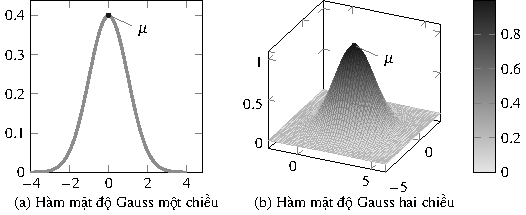
\includegraphics[width=.8\linewidth]{Figs/C1_Gaussian}
%		\begin{flushleft}
%		\it\footnotesize	Chú thích: (a) Hàm mật độ xác suất Gauss trong không gian $\mathbb{R}$, cụ thể là $X\sim\mathcal{N}(0\,;1)$, và (b) trong không gian $\mathbb{R}^2$, $X\sim\mathcal{N}([2\,;-1]^\intercal\,;1.5\bm I_2)$. Nguồn: Minh họa của tác giả
%		\end{flushleft}
%				\caption{Hàm mật độ xác suất Gauss trong các không gian $1$-chiều và $2$-chiều}
%		\label{fig:c1gaussian}
%	\end{figure}

%Hình~\ref{fig:c1gaussian} cho thấy 



Ngoài ra, các phát triển bất đối xứng của Gauss điển hình là hàm Gauss-lệch \cite{azzalini1985class}. với hàm mật độ của nó được định nghĩa như sau.
\dng{[Hàm mật độ Gauss-lệch]
	Biến ngẫu nhiên liên tục $X$ tuân theo mật độ Gauss-lệch (chuẩn-lệch) \cite{azzalini1985class} với ba tham số $\mu$, $\sigma^2$ và $\alpha$ (trong đó $\mu\,;\alpha\in\mathbb{R}$ và $\sigma^2\in\mathbb{R}_{>0}$) nếu nó có hàm mật độ xác suất là
	$$ \mathcal{SN}(x\,;\,\mu\,;\sigma^2\,;\alpha) = \frac{2}{\sqrt{2\pi\sigma^2}}\exp\left(-\frac{(x-\mu)^2}{2\sigma^2}\right)\int^{\alpha(x-\mu)/\sigma}_{-\infty}\frac{1}{\sqrt{2\pi}}\exp\left(-\frac{t^2}{2}\right)\mathrm{\,d}t,\, x \in \mathbb{R}.	 $$
}

Hàm mật độ Gauss-lệch nhận thêm một tham số thể hiện mức độ lệch $\alpha$. Khi giá trị $\alpha$ càng lớn, độ lệch so với kỳ vọng $\mu$ càng lớn. Khi $\alpha = 0$, phân phối này trở về Gauss như Định nghĩa~\ref{dng:Gauss}.

\dly{[Kỳ vọng và phương sai] Kỳ vọng và phương sai của biến ngẫu nhiên $X$ có hàm mật độ xác suất Gauss-lệch là 
	$	\mathbb{E}(X) = \mu + \sigma \delta \sqrt{\frac{2}{\pi}}\,;
		\mathrm{Var}(X) = \sigma^2 \left(1 - \frac{2 \delta^2}{\pi}\right)
		$, với $\delta=\frac{\alpha}{\sqrt{1 + \alpha^2}}$ nằm trong $(-1\,;1)$.
}






\dng{[Hàm mật độ đều]
	Biến ngẫu nhiên liên tục $X$ tuân theo phân phối đều trên đoạn $[l\,;u]$ (với $l < u$ và $l\,; u \in \mathbb{R}$) nếu nó có hàm mật độ xác suất là
	$$
	\mathcal	U(x\,;\,l\,; u) =
	\begin{cases}
		\frac{1}{u- l}, & x \in [l\,; u], \\
		0, & x\notin [l\,;u].
	\end{cases}
	$$
}

	\dly{[Kỳ vọng và phương sai] Kỳ vọng và phương sai của biến ngẫu nhiên $X$ có hàm mật độ xác suất đều là $\mathbb{E}(X) = \frac{l + u}{2}\,; \mathrm{Var}(X) = \frac{(u- l)^2}{12}$.
}

\dng{[Hàm mật độ đều $d$-chiều]
	Biến ngẫu nhiên liên tục $d$-chiều $\bm X$ tuân theo phân phối đều trên hình hộp $[l_1\,; u_1] \times \cdots \times [l_d\,; u_d]$ (với $l_i < u_i$, $l_i\,; u_i \in \mathbb{R}$) nếu nó có hàm mật độ xác suất là
	$$
	\mathcal	U(\bm x\,;\,\bm l\,; \bm u) =
	\begin{cases}
		\prod_{i=1}^d \frac{1}{u_i -l_i}, & \bm x \in [l_1\,; u_1] \times \cdots \times [l_d\,; u_d], \\
		0, & \text{ngược lại}.
	\end{cases}
	$$
}

	\dly{[Kỳ vọng và hiệp phương sai] Kỳ vọng và phương sai của biến ngẫu nhiên $\bm X$ có hàm mật độ xác suất đều là $\mathbb{E}(\bm X) = \frac{\bm{l} + \bm{u}}{2}\,; \mathrm{Cov}(\bm X) = \mathrm{diag}\left(\frac{(u_1 - l_1)^2}{12}, \dots, \frac{(u_d - l_d)^2}{12}\right)$.
}

\section{Một số hàm mật độ bổ sung}
Gần đây, các thuật toán phân tích chùm dựa vào trọng tâm đề xuất bổ sung hàm mật độ xác suất trọng tâm (hay hàm mật độ đại diện của chùm) \cite{nguyentrang2017fuzzy,vovan2019cluster}. Nó có chức năng như trung bình có trọng số của tổng các hàm mật độ trong chùm.

\dng{[Hàm mật độ đại diện chùm]
    Cho tập $\mathcal{F}$ gồm $n$-hàm mật độ xác suất, trong đó, $\mathcal{F}=\{f_1(x)\,;f_2(x)\,;\ldots\,;f_n(x)\}$ với $n\ge 2$. Ta phân bổ $\mathcal{F}$ vào $c$-chùm $(1<c\le n)$, khi này hàm mật độ đại diện của các chùm $c_i$ là 
    \begin{align}\label{daidien}
        \theta_i(x) = \frac{\sum_{j=1}^n\mu_{ij}\times f_j(x)}{\sum_{j=1}^n\mu_{ij}},
    \end{align}
    trong đó, $\mu_{ij}$ là trọng số phân bổ hàm mật độ $f_j(x)$ bất kỳ vào chùm $c_i$ \cite{wald1950statistical}.

}



Dựa vào định nghĩa trên, ta dễ dàng nhận được $\theta_i$ cũng là một hàm mật độ thỏa Tính chất~\ref{tc1}. 
\chm{Các giá trị trọng số $0\le\mu_{ij}\le1$ nên các $\theta_i$ liên tục không âm, và 
$$\int_{\Omega}\theta_i(x)\mathrm{\,d}x=\int_{\Omega}\frac{\sum_{j=1}^n\mu_{ij}\times f_j(x)}{\sum_{j=1}^n\mu_{ij}}\mathrm{\,d}x = \frac{\sum_{j=1}^n\mu_{ij}\times \int_{\Omega}f_j(x)\mathrm{\,d}x }{\sum_{j=1}^n\mu_{ij}} = 1.$$}

\dly{Kỳ vọng của biến ngẫu nhiên $X$ có hàm mật độ xác suất đại diện $\theta_i(x)$ là
	$$
	\mathbb{E}_{\theta_i}(X) = \frac{\sum_{j=1}^n \mu_{ij} \mathbb{E}_{f_j}(X)}{\sum_{j=1}^n \mu_{ij}}.
	$$
}

\chm{Ta có
	\begin{align*}
		\mathbb{E}_{\theta_i}(X)
		= \int_{\Omega} x\, \theta_i(x)\, \mathrm{d}x &= \int _{\Omega}x\, \frac{\sum_{j=1}^n \mu_{ij} f_j(x)}{\sum_{j=1}^n \mu_{ij}}\, \mathrm{d}x = \frac{1}{\sum_{j=1}^n \mu_{ij}} \sum_{j=1}^n \mu_{ij}\underbrace{ \int_{\Omega} x\, f_j(x)\, \mathrm{d}x}_{= \mathbb{E}_{f_j}(X)}.
	\end{align*}
	Từ đây, ta suy ra điều phải chứng minh.
}


Ta cũng mở rộng được cho hàm mật độ đại diện chùm đến không gian $d$-chiều tương tự cho véc-tơ ngẫu nhiên $\bm X$ và nó cũng thỏa mãn các tính chất của một hàm mật độ xác suất. Mới đây, Thao Nguyen-Trang \textit{et al.} \cite{nguyen2023globally,nguyen2023balance} đề xuất hàm mật độ đại diện Gauss như là một phiên bản Gauss hóa của hàm Fréchet \cite{frechet1948elements}. 

\dng{[Hàm mật độ đại diện Gauss] Hàm mật độ đại diện Gauss có dạng phân phối chuẩn sao cho tổng khoảng cách giữa chúng đến các hàm mật độ khác là nhỏ nhất \cite{frechet1948elements}, tức là
$$\theta_i(x) = \arg\min_{\mathcal{N}(\mu\,;\sigma)}\sum_{j=1}^n\mu_{ij}D(\mathcal{N}(\mu\,;\sigma)\,;f_j(x)).$$
trong đó, $D(\mathcal{N}(\mu\,;\sigma)\,;f_j(x))$ là khoảng cách giữa hai hàm mật độ Gauss trong tổng thể. 
}



\chy{	 Hàm mật độ đại diện Gauss là hàm trung bình Fréchet nên có nghiệm duy nhất \cite{frechet1948elements}. Khác với \eqref{daidien}, hàm mật độ này chỉ cần tìm một hàm Gauss duy nhất mà không cần tổ hợp các $f_j$ giúp tăng khả năng khái quát hóa. Ta cũng có phương sai Fréchet $\mathrm{Var}_j(X)=\mathbb{E}(D^2(\mathcal{N}(\mu\,;\sigma)\,;f_j(x)))$.
	}
	
 
 Hình \ref{fig:hamdaidien} minh họa cụ thể hai cách biểu diễn hàm mật độ đại diện trong cùng một chùm hàm Gauss. Dễ thấy sự khác biệt, hàm mật độ đại diện tập trung vào phân bổ trung bình của nó tại các chùm, còn hàm mật độ đại diện Gauss lựa chọn vị trí dựa vào khoảng cách các hàm mật độ với nhau. 

\begin{figure}[H]
	\centering
	    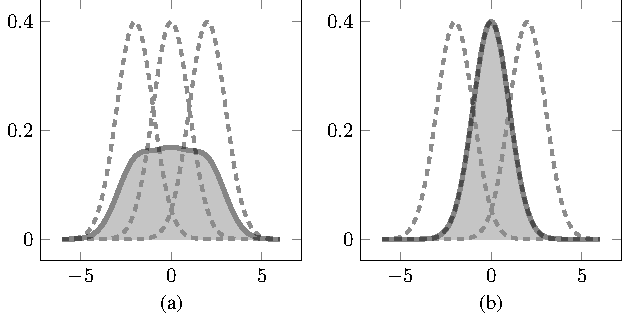
\includegraphics[width=\linewidth]{Figs/C1_hamdaidien.pdf}
	    \begin{flushleft}
	    	\it\footnotesize Chú thích: Hàm mật độ đại diện thể hiện bằng đường thẳng in đậm cho ba hàm Gauss minh họa bằng nét đứt (a) dựa vào trọng số phân bổ đều giữa ba hàm $\mu_{ij}=1/3$, và (b) dựa vào vị trí tối ưu. Ta có thể nói hàm mật độ đại diện này là kỳ vọng của các tổng thể khác nhau. Nguồn: Minh họa của tác giả.
	    \end{flushleft}
	\caption{Minh họa hai hàm mật độ xác suất đại diện một chùm hàm mật độ $\mathcal{F}$.}
	\label{fig:hamdaidien}
\end{figure}


\section{Ước lượng hàm mật độ xác suất}



Trong thực tế, ta cần phải ước lượng hàm mật độ xác suất dựa vào dữ liệu rời rạc, luận văn này sử dụng phương pháp ước lượng hàm hạt nhân để chuyển từ bài toán rời rạc sang hàm mật độ xác suất.
\dng{[Ước lượng hàm mật độ bằng phương pháp hàm hạt nhân]
	Giả sử ta có một tập dữ liệu rời rạc gồm $n$ quan sát ${\bm{x}_j}$ với $j = 1, \ldots, n$ trong không gian $\mathbb{R}^d$. Mỗi điểm $\bm{x}_j = (x_{1j}, x_{2j}, \ldots, x_{dj})^\intercal$. Hàm mật độ xác suất tại điểm $\bm{x} = (x_1, x_2, \ldots, x_d)^\intercal$ được ước lượng bằng phương pháp hạt nhân bởi
	\[
	\hat{f}(\bm{x}) = \frac{1}{n \prod_{i=1}^d {bw}_i} \sum_{j=1}^{n} \prod_{i=1}^{d} \kappa_i\left( \frac{x_i - x_{ij}}{{bw}_i} \right),
	\]
	trong đó $\kappa_i$ là hàm hạt nhân theo chiều $i$ có tính chất $\kappa(\cdot) \ge 0$ và $\int \kappa(z)\mathrm{d}z = 1$, tham số ${bw}_i > 0$ là tham số trơn ứng với chiều đó.
}

\chy{Khi tham số trơn $bw$ nhỏ, hàm mật độ ước lượng sẽ kém trơn và có thể dao động mạnh; ngược lại, nếu $bw$ lớn thì hàm trở nên trơn hơn nhưng có thể làm mất chi tiết quan trọng của phân phối gốc. Trong trường hợp đơn giản, có thể chọn cùng một hàm hạt nhân và cùng một tham số trơn cho tất cả các chiều, tức là $\kappa_i \equiv \kappa$ và ${bw}_i = {bw}$ với mọi $i=1,\ldots,d$. 
	
	Một số hàm hạt nhân phổ biến được liệt kê trong Bảng~\ref{tab:kernel}. Luận văn này khảo sát hàm mật độ ước lượng từ hàm hạt nhân Gauss và Epanechnikov với tham số trơn cố định và được tính bởi công thức của Silverman, $bw = 1.06 \times \mathrm{Var}(x_j) \times n^{-1/5}$.


\begin{figure}[H]
	\centering
	\begin{subfigure}{.48\textwidth}
			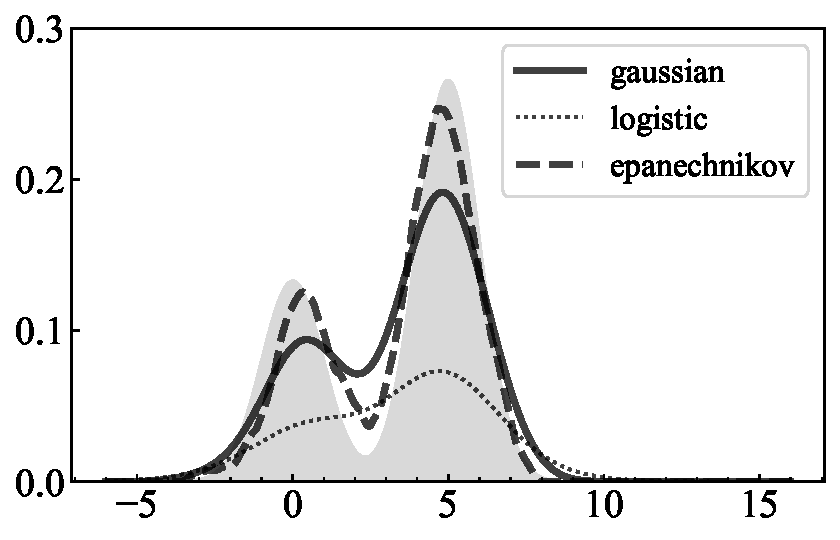
\includegraphics[width=\linewidth]{Figs/C1_kde_kernels.pdf}
			\caption{}
	\end{subfigure}
		\begin{subfigure}{.48\textwidth}
		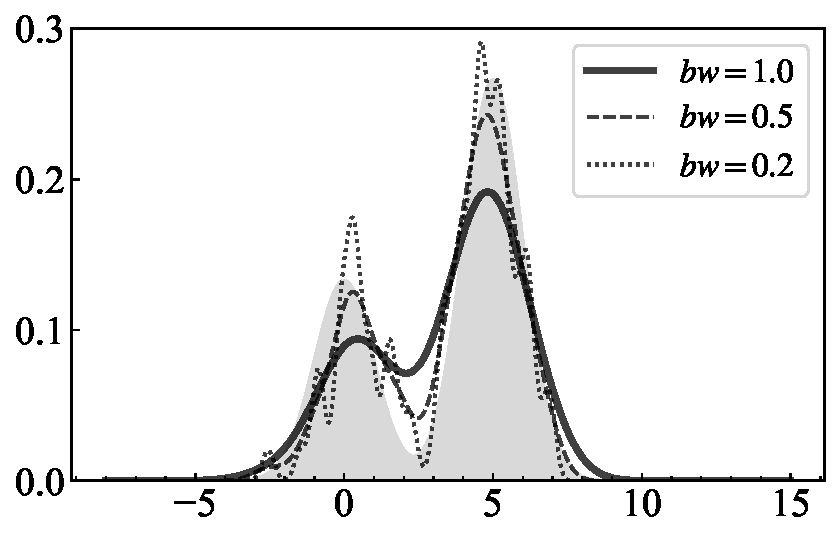
\includegraphics[width=\linewidth]{Figs/C1_kde_bw.pdf}
		\caption{}
	\end{subfigure}
	\begin{flushleft}
		\it\footnotesize
		Chú thích: Vùng xám là phân phối thực tế $X\sim 0,3\mathcal{N}(0\,;1) + 0,7\mathcal{N}(5\,;1)$, (a) các hàm hạt nhân ảnh hưởng đến khả năng khớp với hàm mật độ thực tế, trong khi (b) tham số trơn ảnh hưởng đến mức độ khớp. Nguồn: Minh họa của tác giả.
	\end{flushleft}
	\caption{So sánh các hàm hạt nhân và hệ số trơn trong ước lượng mật độ xác suất}
	\label{fig:kde}
\end{figure}
}





\begin{table}[H]
	\centering
	\caption{Một số hàm hạt nhân phổ biến dùng trong ước lượng mật độ hạt nhân}
	\label{tab:kernel}
	\centering\scriptsize
\begin{tabular*}{\columnwidth}{@{\extracolsep\fill}lllc@{\extracolsep\fill}} 
		\toprule
		\textbf{Tên hàm} & \textbf{$\kappa(z)$} & \textbf{Miền xác định} & \textbf{Khả vi}\\\midrule
		Hình chữ nhật &
		$ (1/2)\bm1_{\{|z| \leq 1\}}$ &
		$[-1\,; 1]$ &  \\
		Tam giác &
		$ (1 - |z|) \bm1_{\{|z| \leq 1\}}$ &
		$[-1\,; 1]$ & $\mathcal{C}^0$ \\
		Epanechnikov &
		$ (3/4)(1 - z^2) \bm1_{\{|z| \leq 1\}}$ &
		$[-1\,; 1]$ &  $\mathcal{C}^0$ \\
		Gauss &
		$ \frac{1}{\sqrt{2\pi}} \exp\left(-z^2/2\right)$ &
	$(-\infty,\infty)$ &  $\mathcal{C}^\infty$  \\
		Logistic &
		$\frac{\exp(-z)}{1 + \exp(-z)^2}$ &
		$(-\infty,\infty)$ & $\mathcal{C}^\infty$\\
		\bottomrule
	\end{tabular*}
\end{table}








\section{Độ đo đánh giá sự tương tự của các hàm mật độ xác suất}

Khoảng cách là độ đo xa-gần các vật thể. Ở đây, khái niệm {\it khoảng cách} bao hàm cả {\it độ đo phân biệt}. 
%Phần này giới thiệu một số loại khoảng cách đối với hai đối tượng hàm mật độ bao gồm: khoảng cách hai hàm mật độ, một hàm mật độ với một chùm hàm và giữa hai chùm hàm mật độ bất kỳ.

\subsection{Sự tương tự của hai hàm mật độ xác suất}

%Cho $f\,;g$ là hai hàm mật độ Radon-Nikodym tương ứng với độ đo trong không gian đo được $(\Omega\,;\mathcal{B})$ với $\mathcal{X}\subseteq \mathbb{\mathbb{R}^d$.
	
 \dng{[Khoảng cách $\mathcal L_p$]\label{D} Cho hai hàm mật độ xác suất $f_1\,; f_2$ trên $\mathbb R^d$. Khoảng cách $\mathcal{L}_p$ được định nghĩa là\[ \mathcal L_p(f,g)=\left(\int_{\mathbb R^d}|f_1(x)-f_2(x)|^p\,\mathrm{d}x\right)^{\!1/p}\,; 1\le p<\infty .\]
}
	
	Theo Định nghĩa \ref{D}, khoảng cách giữa hai hàm mật độ thỏa mãn các tiên đề của mê-tríc. Thực tế, ta thường sử dụng $p=1$ hoặc $p=2$ cho các tính toán. Trong lý thuyết thống kê và thông tin, một mê-tríc được gọi là \emph{khoảng cách} và nửa mê-tríc gọi là \emph{phân kỳ}. Ta cũng có mối quan hệ giữa hai hàm mật độ đối mới trọng tâm bất kỳ trong mê-tríc.

	
	
	
	\bode{[Bất đẳng thức tam giác]
		Với mọi $f_j, f_k \in c_i$ và trọng tâm chùm $\theta_i$ có khoảng cách là mê-tríc, ta có bất đẳng thức tam giác $D(f_j, f_k) \leq D(f_j, \theta_i) + D(f_k, \theta_i).$
	}
	
		Tai Vo-Van (2019) \cite{vovan2019cluster} dựa trên khoảng cách $\mathcal L_p$ để giới thiệu độ rộng chùm.
	$$ CWD(f_1\,;f_2) = \int_{\Omega}\max\{f_1(x)\,;f_2(x)\}\mathrm{\,d}x  - 1$$
	
	

\dng{[$f$-phân kỳ] Hàm $D\,:\,P_1\times P_2\rightarrow \mathbb{R}$ được gọi là $f$-phân kỳ của hai hàm mật độ $f_1\in P_1$ và $f_2\in P_2$ khi nó thỏa hệ số phân kỳ giữa hai xác suất \cite{ali1966general}
$$D(P_1, P_2) = h \left(\mathbb{E}_1 \left(g \left( \frac{f_2}{f_1} \right) \right) \right),$$
	trong đó $g$ là một hàm liên tục lồi trên $\mathbb{R}_{>0}$, $h$ là hàm tăng trên $\mathbb{R}$, và $\mathbb{E}_1$ là kỳ vọng của  $P_1$.
	} 


% Các khoảng cách của hai hàm mật độ xác suất được thành lập theo hai các tiếp cận: véc-tơ và xác suất. Cách tiếp cận véc-tơ xem xét các mức giá trị là điểm trong không gian Euclide, nên chúng cũng có thể tính toán dựa vào các khoảng cách hình học thông thường. 

Bảng~\ref{tab1:KC_PDF} làm rõ các công thức khoảng cách và độ đo tương tự giữa hai hàm mật độ xác suất theo tiếp cận xác suất.
\begin{table}[H]
	\caption{Bảng tổng kết các loại khoảng cách và các chỉ số khác giữa hai hàm mật độ xác suất}\label{tab1:KC_PDF}
	\centering\scriptsize
	\begin{tabular*}{\columnwidth}{@{\extracolsep\fill}lllll@{\extracolsep\fill}} 
		\toprule
		\bf Khoảng cách & \bf $D(f_1(x), f_2(x))$ & \bf $g(u)$ & \bf $h(u)$ & \bf Miền giá trị  \\ \midrule
		$\mathcal{L}_1$ & $\displaystyle\int_{\Omega}|f_1(x) - f_2(x)|\mathrm{\,d}x$ & $|1-u|$ & $u$ & $[0\,;2]$ \\
		Chernoff & $-\log\left(\displaystyle\int_{\Omega} f_1(x)^s f_2(x)^{1-s}\mathrm{\,d}x\right)$ & $-u^{1-s}$ & $-\log(-u)$ & $[0\,;+\infty)$ \\
		Matusita & $\left(\displaystyle\int_{\Omega}\left|f_1^{1/r}(x) - f_2^{1/r}(x)\right|^r\mathrm{\,d}x\right)^{1/r}$ & $\left|1-u^{1/r}\right|^{r}$ & $u^{1/r}$ & $[0\,; \sqrt{2}]$ \\
		bình phương Hellinger & $\displaystyle\int_{\Omega}\left(\sqrt{f_1(x)}-\sqrt{f_2(x)}\right)^2\mathrm{\,d}x$ & $(\sqrt{u}-1)^2$ & $u$ & $[0\,;2]$ \\
		thông tin Kullback&$\displaystyle\int_{\Omega} f_1(x)\log\frac{f_1(x)}{f_2(x)}\mathrm{\,d}x$ & $-\log(u)$ & $u$ & $[0\,;+\infty)$ \\
		 Jensen-Shannon & $\frac{1}{2}\left(D_{KL}(f_1\,; f_2) + D_{KL}(f_2\,; f_1)\right)$ & $-(u+1)\log(\frac{u+1}{2})+u\log(u)$ & $\frac{1}{2}u$ & $[0\,;+\infty)$ \\
	Bayes	Error &$1-\displaystyle\int_{\Omega} \min\{\pi f_1(x)\,;\pi(1-f_2(x))\}\mathrm{\,d}x$ &$-\min\{u\,;1-u\}$ & $u+1$ & $[0\,;1]$ \\
		\bottomrule
	\end{tabular*}
	\\\hfill {\footnotesize Trong khoảng cách Chernoff, $0\le r\le 1$, và \textit{Nguồn: Tác giả tổng hợp}}
\end{table}



\chy{Nhìn vào Bảng \ref{tab1:KC_PDF}, có thể thấy khoảng cách Chernoff là một tổng quát hóa của khoảng cách Bhattacharyya khi chọn $s = 1/2$. Tương tự khoảng cách Matusita là tổng quát hóa của bình phương Hellinger khi $r=2$. Trong $\mathcal{L}_p$, chỉ có $\mathcal{L}_1$ là một $f$-phân kỳ và là Matusita với $r=1$. Đáng chú ý, Matusita thỏa mãn tính chất mê-tríc.
}

Ở Hình~\ref{fig:dayKC}, luận văn này ghi nhận giá trị khoảng cách $f_1\sim\mathcal{N}(0\,;1)$ và $f_2\sim \mathcal{N}(\mu\,;1)$ với $\mu$ trượt từ $-10$ đến $20$.

\begin{figure}[h]
    \centering
\begin{subfigure}{.48\linewidth}
	    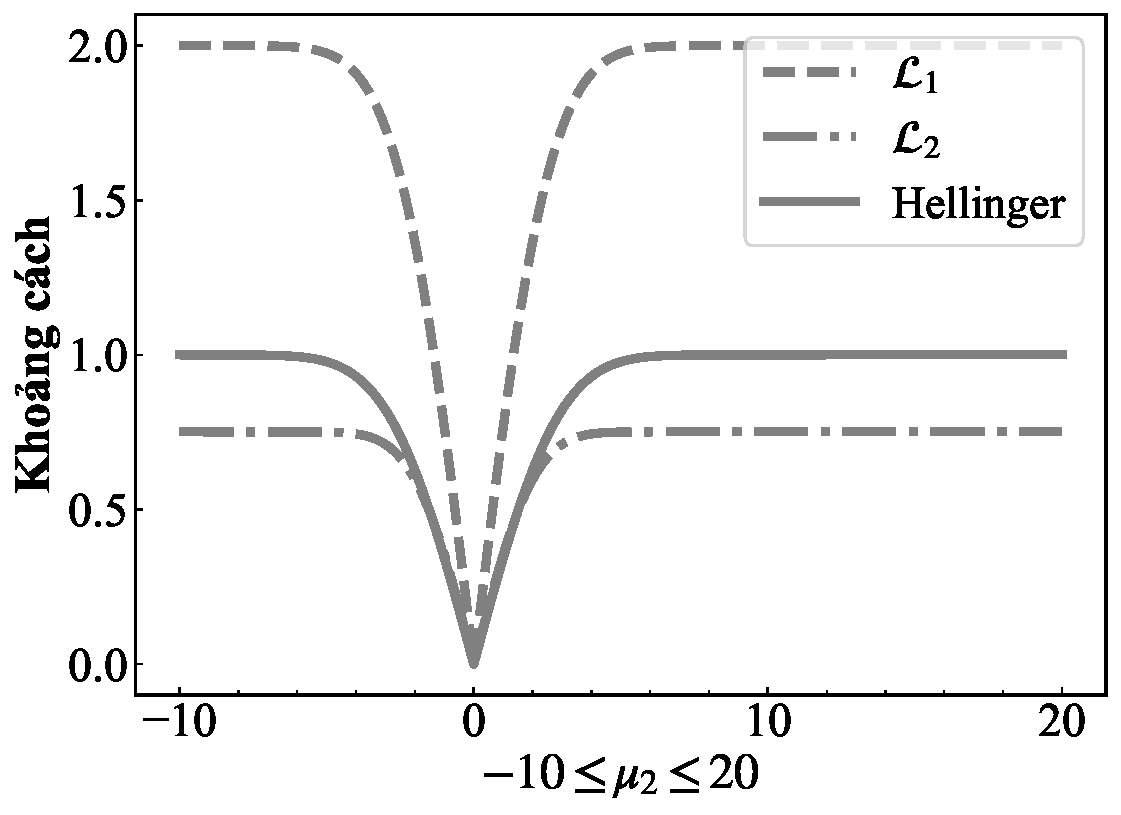
\includegraphics[width=\linewidth]{Figs/C1_dist.pdf}
\caption{}
\end{subfigure}
\begin{subfigure}{.48\linewidth}
	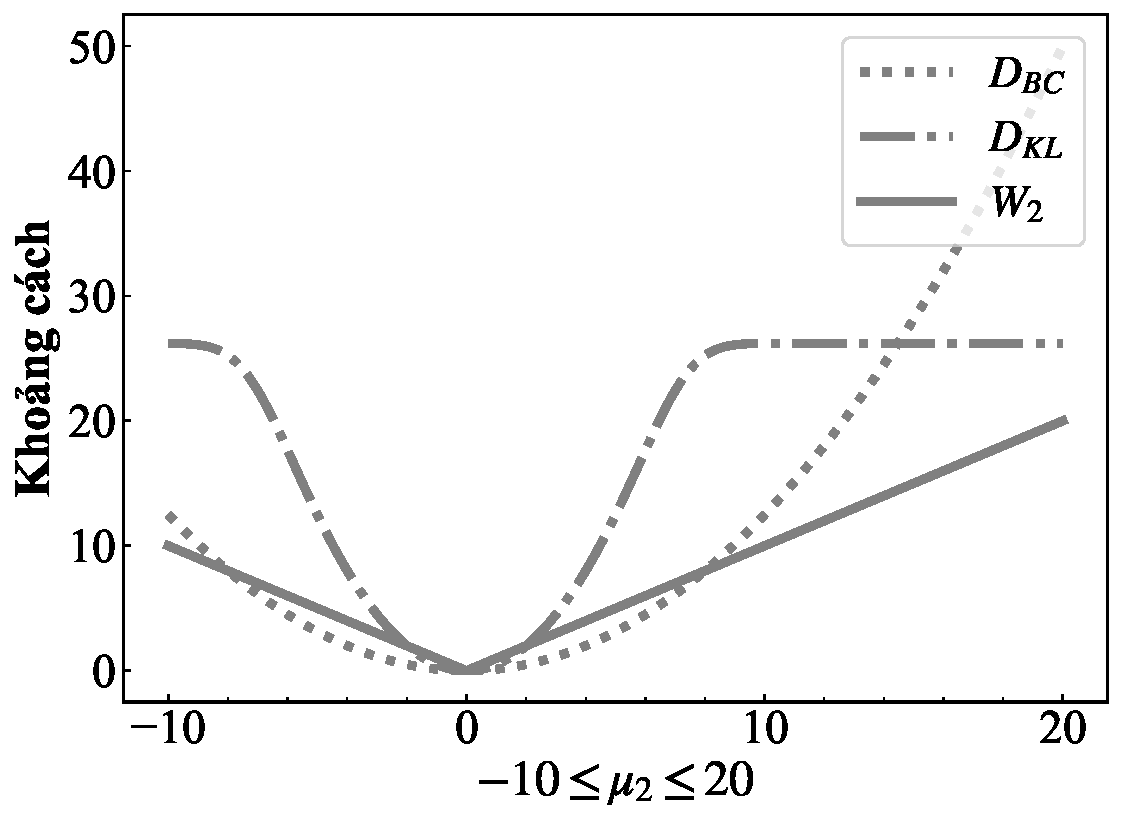
\includegraphics[width=\linewidth]{Figs/C1_dist2.pdf}
	\caption{}
\end{subfigure}
   \begin{flushleft}
   	 {\footnotesize \textit{(a) Các khoảng cách có miền xác định bị chặn trên, (b) ngược lại. Nguồn: Minh họa của tác giả}}
   \end{flushleft}
    \caption{Dãy khoảng cách $D(f_1\,;f_2)$ giữa hai hàm mật độ Gauss $\mathcal{N}(0\,;1)$ và $\mathcal{N}(\mu\,;1)$}
    \label{fig:dayKC}
\end{figure}


\chy{Ta thấy khi hai hàm mật độ $f_2$ cách nhau quá xa hàm $f_1$, tức là $|\mu_2|\gg0$, tất cả loại khoảng cách  hàm mật độ đều bão hòa và không đo được sự khác biệt. Lúc này hai hàm mật độ về mặt không gian rất xa nhau, nhưng khoảng cách không thể đo xa hơn nữa vì nó đã đạt đến ngưỡng lớn nhất. Đây là hạn chế không giữ được vị trí hình học đối với các khoảng cách hàm mật độ.
	}

Luận văn này giới thiệu khoảng cách Wasserstein (hay Kantorovich–Rubinstein), là một mê-tríc hỗ trợ tốt cho tính toán khoảng cách các hàm mật độ không chồng lấp \cite{villani2008optimal} thỏa Định nghĩa~\ref{D} và bất đẳng thức tam giác. Khoảng cách này được phát triển trong bài toán vận chuyển tối ưu\index{vận chuyển tối ưu (optimal transport)}, nhưng chưa được nghiên cứu trong lĩnh vực nhận dạng hàm mật độ.
\dng{[Khoảng cách $p$-Wasserstein]
Khoảng cách $p$-Wasserstein ($p\ge1$) giữa hai độ đo xác suất $\mu$ và $\nu$ trong không gian $\mathbb{R}^d$ được định nghĩa là $$W_p(\mu, \nu) = \inf_{\substack{X \sim \mu \\ Y \sim \nu}} \left( \mathbb{E} \| X - Y \|^p \right)^{1/p}
= \left( \inf_{\gamma \in \Gamma(\mu, \nu)} \int_{M \times M} d(x, y)^p \mathrm{\,d}\gamma(x, y) \right)^{1/p},
$$
}

Khoảng cách $p$-Wasserstein  đo mức chênh lệch tối ưu giữa hai phân phối xác suất, xét trên tất cả các phép ghép cặp khả dĩ. Tức là nó tính đến công sức để di chuyển và tái sắp xếp khối lượng từ hàm này sang hàm kia. Ở đây, luận văn này sử dụng $p=2$ để tính toán đo độ khác biệt giữa hai mật độ xác suất liên tục. Trong thực tế, ta tính toán cụ thể khoảng cách này bằng cách biểu diễn nó qua hàm phân vị. Ta có Định lý~\ref{dly:phanvi}.

\dly{\label{dly:phanvi}
	Khoảng cách $p$-Wasserstein giữa hai độ đo xác suất $\mu$ và $\nu$ có thể được biểu diễn dưới dạng phân vị trong trường hợp $1$-chiều bởi định nghĩa
	$$
	W_p^p(\mu, \nu) = \int_0^1 \left| F_\mu^{-1}(s) - F_\nu^{-1}(s) \right|^p \,\mathrm{d}s,
	$$
	trong đó $F_\mu^{-1}$ và $F_\nu^{-1}$ lần lượt là hàm phân vị của $\mu$ và $\nu$ (Xem Định nghĩa~\ref{dng:hamphanvi}).
}

\dly{[Khoảng cách $2$-Wasserstein giữa hai hàm mật độ Gauss 1 chiều]
	Giả sử hai hàm mật độ $f_1(x) \sim \mathcal{N}(\mu_1, \sigma_1^2)$ và $f_2(x) \sim \mathcal{N}(\mu_2, \sigma_2^2)$ là hai phân bố Gauss một chiều. Khi đó, khoảng cách $2$-Wasserstein giữa chúng là
	$
	D_{W}^2(f_1, f_2) = (\mu_1 - \mu_2)^2 + (\sigma_1 - \sigma_2)^2.
	$
}




\chm{Dựa vào Định lý~\ref{dly:phanvi}, ta xét hàm phân vị Gauss $F_i^{-1}(u)= \mu_i + \sigma_i \Phi^{-1}(u),
	$ với $\Phi^{-1}(u)$ là phân vị chuẩn $\mathcal{N}(0,1)$. Khi đó,
	\begin{align*}
		D_{W}^2(f_1, f_2) 
		&= \int_0^1 \left( \mu_1 + \sigma_1 \Phi^{-1}(u) - \mu_2 - \sigma_2 \Phi^{-1}(u) \right)^2 \mathrm{\,d}u \\
		&= \int_0^1 \left( (\mu_1 - \mu_2) + (\sigma_1 - \sigma_2) \Phi^{-1}(u) \right)^2 \mathrm{\,d}u \\
	&= \int_0^1 \Big[ 
	(\mu_1 - \mu_2)^2 
	+ 2(\mu_1 - \mu_2)(\sigma_1 - \sigma_2)\Phi^{-1}(u) 
	+ (\sigma_1 - \sigma_2)^2 (\Phi^{-1}(u))^2 
	\Big] \,\mathrm{d}u \\
	&= (\mu_1 - \mu_2)^2 \underbrace{\int_0^1 \mathrm{d}u}_{=1} 
	+ 2(\mu_1 - \mu_2)(\sigma_1 - \sigma_2) \underbrace{\int_0^1 \Phi^{-1}(u)\,\mathrm{d}u}_{=0} 
	+ (\sigma_1 - \sigma_2)^2 \underbrace{\int_0^1 (\Phi^{-1}(u))^2\,\mathrm{d}u}_{=1}.
	\end{align*}
Từ đây ta suy ra được điều phải chứng minh.
}

Tương tự ta cũng suy ra được Định lý khoảng cách sau.

\dly{[Khoảng cách $2$-Wasserstein giữa hai hàm mật độ Gauss $d$-chiều]
	Giả sử hai hàm mật độ $f_1(x) \sim \mathcal{N}(\mu_1, \Sigma_1)$ và $f_2(x) \sim \mathcal{N}(\mu_2, \Sigma_2)$ là hai phân bố Gauss trong $\mathbb{R}^d$. Khi đó, khoảng cách $2$-Wasserstein giữa chúng là
	$$
	D_{W}^2(f_1, f_2) = \|\mu_1 - \mu_2\|_2^2 + \mathrm{Tr}\left(\Sigma_1 + \Sigma_2 - 2(\Sigma_2^{1/2} \Sigma_1 \Sigma_2^{1/2})^{1/2}\right).
	$$
}



\dly{[Khoảng cách $2$-Wasserstein giữa hai phân phối đều $1$-chiều] Giả sử hai hàm mật độ  $f_1(x) \sim \mathcal{U}[a_1, b_1]$ và $f_2(x) \sim \mathcal{U}[a_2, b_2]$ là hai phân phối đều một chiều. Khi đó, khoảng cách $2$-Wasserstein giữa chúng là
		$
	D_{W}^2(f_1, f_2) = (\mu_1 - \mu_2)^2 + \frac{1}{12}(l_1-l_2)^2,
	$
	trong đó $m_i = \frac{a_i + b_i}{2}$ là trung điểm và $l_i = b_i - a_i$ là độ dài của khoảng $[a_i, b_i]$.}



\vdu{[So sánh các loại khoảng cách hàm mật độ] Xét hai hàm mật độ xác suất đều $f_1(x)$ và $f_2(x)$. Hình~\ref{fig:daydeu} mô tả bốn tình huống khoảng cách giữa hai hàm mật độ này.
	\begin{figure}[H]
		\centering
		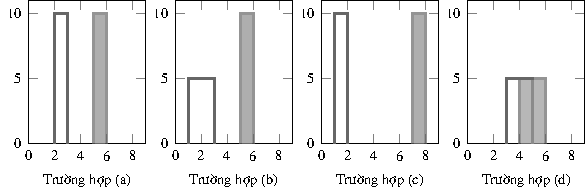
\includegraphics[width=\linewidth]{Figs/C1_Uniform.pdf}
		\begin{flushleft}
		% Chú thích giải thích
		\footnotesize \it Chú thích: Bốn trường hợp mật độ đều với (a) hai hàm rời nhau, cùng chiều rộng; (b) hai hàm rời nhau, khác chiều rộng; (c) hai hàm rời nhau, cách xa nhau; và (d) hai hàm chồng lấp. Ở đây, ô vuông trắng \begin{tikzpicture}
			\node[draw=black,line width=1pt,opacity=0.7,fill=black!5, minimum size=3mm] () {};\end{tikzpicture} biểu thị hàm mật độ $f_1(x)$ và ô vuông xám  \begin{tikzpicture}
			\node[draw=black,line width=1pt,opacity=0.7, fill=black!75, minimum size=3mm] () {};\end{tikzpicture}  biểu thị hàm mật độ $f_2(x)$. Nguồn: Minh họa của tác giả.
		\end{flushleft}
		\caption{Các trường hợp trong khoảng cách giữa hai hàm mật độ đều $f_1(x)$ và $f_2(x)$.}\label{fig:daydeu}
		
	\end{figure}
	

Ta có Bảng~\ref{tab:vidusosanh} tổng hợp kết quả các phép đo này trong bốn tình huống. 
\begin{table}[H]
	\caption{Các kết quả khoảng cách giữa hai hàm mật độ đều}
	\label{tab:vidusosanh}
	\centering\scriptsize
	\begin{tabular*}{\columnwidth}{@{\extracolsep\fill}llcccc@{\extracolsep\fill}}
		\toprule
		\multirow{2}{*}{Nhóm}            & \multirow{2}{*}{$D(f_1\,;f_2)$} &          \multicolumn{4}{c}{Trường hợp}          \\ \cmidrule{3-6}
		                                 &                                 &    (a)     &    (b)    &    (c)     &    (d)     \\ \midrule
		\multirow{3}{*}{$\mathcal{L}_p$} &         $\mathcal{L}_1$         &   2{,}00   &  2{,}00   &   2{,}00   &   1{,}00   \\
		                                 &         $\mathcal{L}_2$         &   1{,}41   &  1{,}22   &   1{,}41   &   0{,}71   \\
		                                 &         $D_O$ (Overlap)         &   1{,}00   &  1{,}00   &   1{,}00   &   0{,}50   \\
		                                 &              $CWD$              &   1{,}00   &  1{,}00   &   1{,}00   &   0{,}50   \\ \midrule
		\multirow{6}{*}{$f$-phân kỳ}           &     $D_{B}$ (Bhattacharyya)      &  $\infty$  & $\infty$  &  $\infty$  &   0{,}69   \\
		                                 &        $D_H$ (Hellinger)        &   1{,}00   &  1{,}00   &   1{,}00   &   0{,}71   \\
		                                 &        $D_M$ (Matusita)         &   1{,}41   &  1{,}41   &   1{,}41   &   1{,}00   \\
		                                 &   $D_{KL}$ (Kullback–Leibler)   &  27{,}63   &  27{,}28  &  27{,}63   &  13{,}47   \\
		                                 &    $D_{JS}$ (Jensen–Shannon)    &  27{,}63   &  26{,}94  &  27{,}63   &  13{,}47   \\ \midrule
		Optimal                          &     $D_{W}$ (2-Wasserstein)     & \bf 3{,}00 & \bf 3{,}5 & \bf 6{,}00 & \bf 1{,}00 \\ \bottomrule
	\end{tabular*}
\end{table}

Trước hết, các khoảng cách $\mathcal{L}_1$ và $\mathcal{L}_2$ trong các trường hợp (a), (b), và (c), mặc dù $f_1(x)$ và $f_2(x)$ nằm xa dần, nhưng các giá trị $\mathcal{L}_1$ và $\mathcal{L}_2$ hầu như không đổi (đều bằng 2 hoặc $\sqrt{2}$). Khoảng cách này nhận biết được khác biệt hình dáng và phân bố, nhưng không nhận biết tốt yếu tố vị trí trong không gian. Hệ số Bhattacharyya và khoảng cách Hellinger chỉ có ý nghĩa trong trường hợp (d), khi có phần chồng lấp giữa $f_1(x)$ và $f_2(x)$. Điều này cho thấy chúng nhạy với mức độ chồng lấp, nhưng không phân biệt được hai hàm độc lập nhau. 

Ngược lại, khoảng cách Wasserstein nhạy cảm với vị trí hình học, hình dáng và phân bố. Khi so (a) và (c), ta thấy khoảng cách này tăng rất lớn cho thấy hiệu quả so sánh vị trí. Xét (a) và (b), khi thay đổi hình dáng hàm mật độ, khoảng cách này cũng có sự khác biệt. Đáng chú ý, khoảng cách $\mathcal{L}_2$ và $D_W$ là trái ngược nhau. Khi thay đổi hình dáng đồ thị, khoảng cách $\mathcal{L}_2$ giảm nhưng $D_W$ lại tăng lên. Cuối cùng, trường hợp (d) cho thấy khoảng cách cũng có ý nghĩa khi chồng lấp. 
}

%Ta tiếp tục định nghĩa các khái niệm liên quan đến khoảng cách hai hàm mật độ.

\dng{[Affinity] Hàm $\rho\,:\,f\rightarrow [0\,;1]$ được gọi là affinity của hai hàm mật độ $f_1(x)$ và $f_2(x)$ nếu nó thỏa mãn ba điều kiện
	\begin{enumerate}
		\item $0\le \rho(f_1\,;f_2) \le1$,
		\item $\rho(f_1\,;f_2) = 1$ nếu và chỉ nếu $f_1\equiv f_2$, và
		\item mỗi dãy hàm $\{f_n\}$ thì $\rho(f_n\,;f_0)\rightarrow 1$ 
	\end{enumerate}
}

\chy{ Affinity đo lường sự giống nhau giữa hai hàm mật độ theo vị trí. Vì vậy, ta có tương quan giữa Affinity và Khoảng cách giữa hai hàm mật độ xác suất $f_1(x)$ và $f_2(x)$ là $D(f_1\,;f_2) = 1-\rho(f_1\,;f_2)$.}

\vdu{
	Affinity cơ bản cho tương tự hai hàm mật độ $f_1(x)$ và $f_2(x)$ là Affinity Bhattacharyya\index{Affinity Bhattacharyya} với 
	$
	\rho_B(f_1, f_2) = \int_\Omega \sqrt{f_1(x) f_2(x)}\mathrm{\,d}x.
	$
}

\dng{[Hàm hạt nhân của khoảng cách]  Hàm
	$
	K\,:\, \mathcal{F} \times \mathcal{F} \to [0\,;1]
	$ với tập $\mathcal{F}$	được gọi là hạt nhân (hạch) giữa hai hàm mật độ $f_1(x), f_2(x)$ nếu nó thỏa mãn
	\begin{enumerate}
		\item $0 \leq K(f_1, f_2) \leq 1$,
		\item $K(f_1, f_2) = K(f_2, f_1)\,; \forall f_1, f_2 \in \mathcal{F}$,
		\item với mọi tập hữu hạn $\{f_1\,; \ldots\,; f_n\} \subset \mathcal{F}$ và các hệ số $\alpha_1\,;\ldots\,;\alpha_n \in \mathbb{R}$, hàm hạt nhân là xác định dương, tức là 
		$
		\sum_{i=1}^n \sum_{j=1}^n \alpha_i \alpha_j K(f_i, f_j) \geq 0.
		$
	\end{enumerate}
}

\vdu{
Ba hạt nhân cơ bản cho khoảng cách hai hàm mật độ $f_1(x)$ và $f_2(x)$ là 
\begin{enumerate}
	\item Hạt nhân chuẩn\index{hạt nhân chuẩn (Gaussian kernel)}, 
	$
	K_G(f_1, f_2) = \exp(-\frac{\mathcal{L}_p^2(f_1, f_2)}{\beta\sigma^2})\,; \beta \in \mathbb{R}_{>0},
	$
	
	\item Hạt nhân tuyến tính \index{hạt nhân tuyến tính (Linear kernel)}, 
	$
	K_L(f_1, f_2) = \int_\Omega f_1(x)f_2(x)\,\mathrm{d}x,
	$
	
	\item Hạt nhân Bhattacharyya \index{Hạt nhân Bhattacharyya}, 
	$
	K_B(f_1, f_2) = \int_\Omega \sqrt{f_1(x) f_2(x)}\,\mathrm{d}x,
	$
	
	\item Hạt nhân \(\chi^2\)\index{Hạt nhân \(\chi^2\) (Chi-squared kernel)}, 
	$
	K_{\chi^2}(f_1, f_2) = \int_\Omega \frac{2f_1(x)f_2(x)}{f_1(x) + f_2(x)}\,\mathrm{d}x.
	$
\end{enumerate}
}

Hàm hạt nhân $K(\cdot\,;\cdot)$ càng gần 1 thì hai hàm mật độ càng giống nhau và ngược lại. Ở đây, việc chuyển đổi từ hàm hạt nhân đến khoảng cách được cho bởi $D = 1-K_G$ khi các hạt nhân chuẩn hóa $[0\,;1]$, hoặc $D=2(1-K_H)$ khi là hạt nhân Bhattacharyya.

\dng{[Ma trận khoảng cách từng đôi]
	Cho tập $n$ hàm mật độ $\{f_1, f_2, \dots, f_n\}$, ma trận khoảng cách $\bm D \in \mathbb{R}^{n \times n}$ là một ma trận đối xứng và có $\mathrm{Trace}(\bm D)=0$, được định nghĩa bởi $
	\bm D_{ij} = D(f_i, f_j)$, với mọi $i,j =1,\dots,n$.
}

\subsection{Sự tương tự của nhiều hơn hai hàm mật độ xác suất}

\subsubsection{a.\quad Liên kết chùm hàm mật độ}

Giả sử hai chùm hàm mật độ không rỗng $\mathcal{F}$ và $\mathcal{G}$ chứa hữu hạn phần tử và $D(f\,;g)$ là khoảng cách giữa hai hàm mật độ, $f\in\mathcal{F}$ và $g\in\mathcal{G}$. Khoảng cách giữa hai chùm hàm mật độ gọi là \emph{liên kết}, là một ánh xạ $\delta\,:\, {\mathcal {P}\!\left( {X}\right) } \times {\mathcal {P}\left( {X}\right) } \times \mathcal {M}(X) \to \mathbb {R}_+$, trong đó, $\mathcal{P}(X)$ là tập lũy thừa của $X$.

\begin{table}[H]
\caption{Bảng tổng kết các loại liên kết $\Delta$ giữa hai chùm hàm mật độ xác suất}
	\centering\scriptsize
	\begin{tabular*}{\columnwidth}{@{\extracolsep\fill}lll@{\extracolsep\fill}} 
			\toprule
			\bf Liên kết &\bf Ký hiệu & \bf                             $\Delta$                             \\ \midrule
			Liên kết đơn\footnotemark[1] (SLINK)\citep{florek1951liaison}&$\Delta_{\min}$&$\min_{f\in\mathcal{F}, g\in\mathcal{G}}D(f\,;g)$\\
			Liên kết đủ\footnotemark[2] (CLINK)\citep{sorensen1948method} &$\Delta_{\max}$& $\max_{f\in\mathcal{F}, g\in\mathcal{G}}D(f\,;g)$\\
			Liên kết tâm (UPGMC)&$\Delta_{centroid}$&$D(\theta_{\mathcal{F}}\,;\theta_{\mathcal{G}})$\\
			Liên kết trung bình (UPGMA)&$\Delta_{avg}$ & $\frac{1}{\#\mathcal{F}\#\mathcal{G}}\sum_{f\in\mathcal{F}, g\in\mathcal{G}}D(\mathcal{F}\,;\mathcal{G})$\\
			Liên kết Ward \cite{ward1963hierarchical}&$\Delta_{Ward}$ &$\frac{\#\mathcal{F} \cdot \#\mathcal{G}}{\#\mathcal{F} + \#\mathcal{G}} D^2\big(\theta_{\mathcal{F}},\, \theta_{\mathcal{G}}\big)
			$\\ \bottomrule
		\end{tabular*}
		\\\hfill {\footnotesize \textit{Chú thích: \footnotemark[1]: tổng khoảng cách nhỏ nhất; \footnotemark[2]: tổng khoảng cách lớn nhất. Nguồn: Tác giả tổng hợp}}
\end{table}


%\begin{figure}[H]\footnotesize
%	 \centering
%	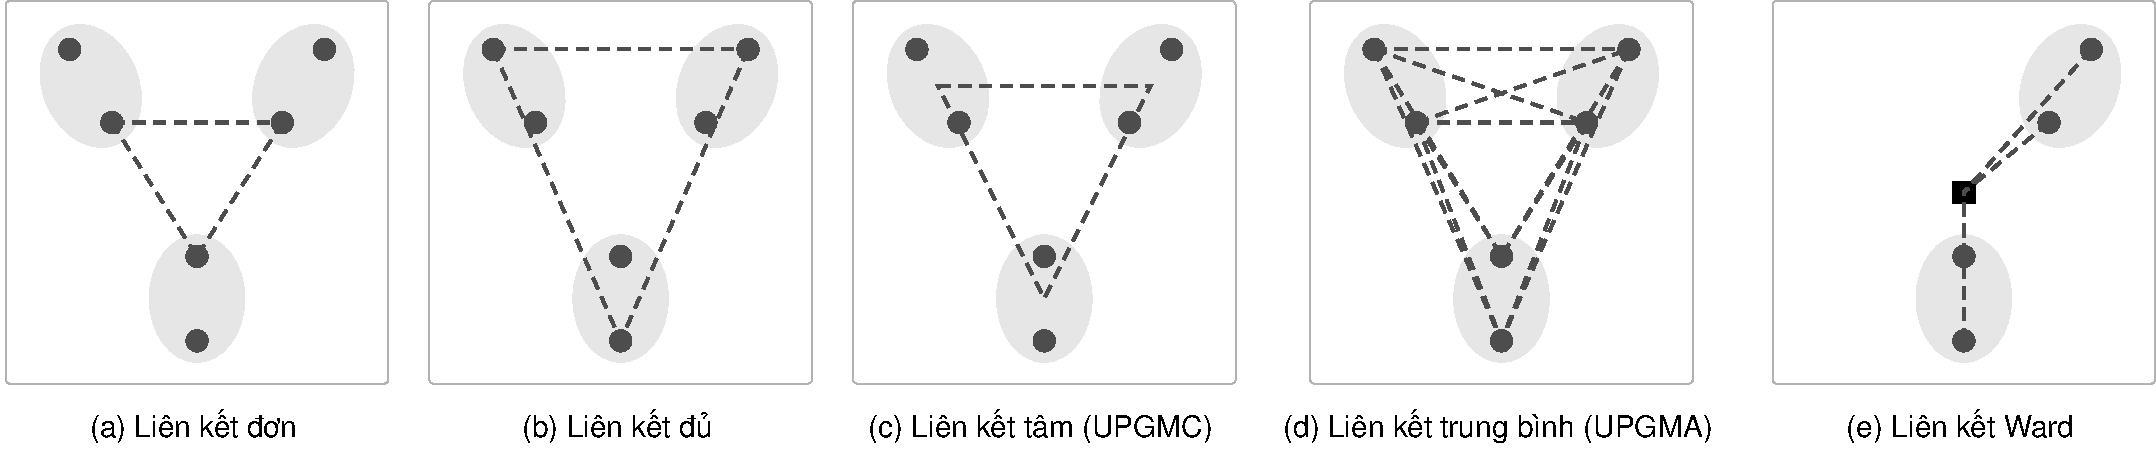
\includegraphics[width=\linewidth]{Figs/C1_Linkage.pdf}
%	\begin{flushleft}
%	\footnotesize	{\it Chú thích: Các loại liên kết này giữa ba chùm hàm mật độ dựa trên (a) tổng khoảng cách nhỏ nhất, (b) tổng khoảng cách lớn nhất, (c) tổng khoảng cách giữa các hàm mật độ trọng tâm, (d) trung bình cộng tất cả các khoảng cách, (e) khoảng cách tối ưu có tổng bình phương các khoảng cách là lớn nhất. Nguồn: Tác giả vẽ lại từ Gao et al. \cite{gao2023overview}}
%	\end{flushleft}
%	\caption{Các loại liên kết giữa các chùm hàm mật độ xác suất.}
%	\label{fig:linkage}
%\end{figure}


Khi hai ta cần tính khoảng cách từ hợp hai chùm hàm $\mathcal{F}\cup\mathcal{G}$ đến một chùm hàm $\mathcal{H}$, ta cũng có thể sử dụng các loại liên kết trên. Trong thực tế, các liên kết $\Delta$ được biến đổi thành
\begin{align*}
	\Delta_{\min}(\mathcal{F} \cup \mathcal{G},\, \mathcal{H}) &= \min\big\{D_{f\in\mathcal{F}, h\in\mathcal{H}}(f,\, h),\, D_{f\in\mathcal{G}, h\in\mathcal{H}}(g,\, h)\big\}, \\
	\Delta_{\max}(\mathcal{F} \cup \mathcal{G},\, \mathcal{H}) &= \max\big\{D_{f\in\mathcal{F}, h\in\mathcal{H}}(f,\, h),\, D_{f\in\mathcal{G}, h\in\mathcal{H}}(g,\, h)\big\}, \\
	\Delta_\mathrm{avg}(\mathcal{F} \cup \mathcal{G},\, \mathcal{H}) &= \frac{1}{\#(\mathcal{F}\cup\mathcal{G}) \cdot \#\mathcal{H}} \sum_{\substack{f \in \mathcal{F} \cup \mathcal{G}\\ h \in \mathcal{H}}} D(f,\, h), \\
	\Delta_\mathrm{centroid}(\mathcal{F} \cup \mathcal{G},\, \mathcal{H}) &= D\big(\theta_{\mathcal{F} \cup \mathcal{G}},\, \theta_{\mathcal{H}}\big), \\
	\Delta_\mathrm{Ward}(\mathcal{F} \cup \mathcal{G},\, \mathcal{H}) &= \frac{\#(\mathcal{F}\cup\mathcal{G})\cdot \#\mathcal{H}}{(\#\mathcal{F} \cup \#\mathcal{G}) \cup \#\mathcal{H}} D^2\big(\theta_{\mathcal{F} \cup \mathcal{G}},\, \theta_{\mathcal{H}}\big).
\end{align*}

Ví dụ~\ref{VD:dist} cung cấp hướng dẫn tính toán các liên kết $\Delta$ được trình bày ở Phụ lục B, tr.~\pageref{phulucB}.

\subsubsection{b.\quad Tương tự chùm hàm mật độ}

Giả sử tập hợp $\mathcal{F}$ có nhiều hơn hai phần tử $(n>2)$

\begin{table}[H]
	\centering\scriptsize
    \caption{Tổng kết các tương tự giữa các chùm hàm mật độ xác suất}\label{tab:chumham}
	\begin{tabular*}{\columnwidth}{@{\extracolsep\fill}ll@{\extracolsep\fill}} 
			\toprule
			\bf Tương tự & \bf                             $\Delta(\mathcal{F})$                             \\ \midrule
            Affinity của Matusita \cite{matusita1967notion} & $\int_{\Omega}\left(\prod_{j=1}^nf_j(x)\right)^{1/n}\mathrm{\,d}x$\\
            Affinity của Toussaint \cite{toussaint1972some} & $\int_{\Omega}\left(\prod_{j=1}^nf_j(x)\right)^{\alpha_j}\mathrm{\,d}x$\\
			Độ rộng chùm \citep{Tai2010} & $\int_\Omega f_{\max}(x)\mathrm{\,d}x -1$\\
			Hệ số tương tự chùm \cite{vovan2018similar}& $\frac{k}{k-1}\left(1-\frac{1}{k}\int_{\Omega}f_{\max}(x)\mathrm{\,d}x\right)$\\
			\bottomrule
		\end{tabular*}
        \\
        \hfill {\footnotesize \textit{Nguồn: Tác giả tổng hợp}}
\end{table}

\chy{Trong Bảng \ref{tab:chumham} Affinity Toussaint suy biến thành Affinity Matusita khi $\alpha_1=\alpha_2=\cdots=\alpha_n=\frac{1}{n}$. Khi Affinity của Matusita có $n=2$ thì nó trở thành hệ số Bhattacharyya. Cuối cùng, hệ số tượng tự chùm chuẩn hóa tuyến tính độ rộng chùm.}

\section{Phương pháp số xấp xỉ tích phân}

Các tích phân trong lĩnh vực hàm mật độ cần xấp xỉ bằng phương pháp số. Luận văn này, chọn sử dụng phương pháp hình thang\index{phương pháp hình thang (trapezoidal method)} nhằm cải thiện độ chính xác so với tổng Riemann nhưng cũng không tốn quá nhiều tài nguyên như Monte Carlo hay Simpsons. Một tích phân trên miền $\Omega \subset \mathbb{R}^d$ được xấp xỉ bằng công thức tổng quát
$ \int_{\Omega}f(x)\mathrm{\,d}x = \lim_{h\to0}\sum_{i}h^d w_if(x)$. Khi này, giả sử hàm $f\,:\,[a\,;b]\to \mathbb{R}$, chia đoạn $[a\,;b]$ thành $n$, phương pháp hình thang một chiều xấp xỉ tích phân
	\[
	\int_a^b f(x)\, dx \approx \frac{h}{2} \left( f(x_0) + 2 \sum_{i=1}^{n-1} f(x_i) + f(x_n) \right),
	\]
trong đó $x_i = a + ih$, $i=0,\dots,n$. 






%
%\section{Một số định lý hội tụ}
%


%\subsection{Nhân tử L'Arange}
%
%\subsection{Điều kiện Karush–Kuhn–Tucker}
%
%
%
%\subsection{Định lý hội tụ toàn cục Zangwill}
%
%
%
%
%
%
%\begin{theorem}[Định lý Zangwill]
%    
%\end{theorem}





%\newpage

\section{Phân tích chùm cho hàm mật độ xác suất}


\subsection{Phân tích chùm không mờ}	

Phân tích chùm không mờ (hay phân chùm cứng) yêu cầu một phần tử chỉ thuộc duy nhất một chùm cố định. Tiểu mục này trình bày hai khía cạnh chính của phân tích chùm bao gồm phân tích chùm phân vùng (dựa trên trọng tâm) và phân cấp thứ bậc. 



\subsubsection{a.\quad Phân tích chùm $k$-means (KCF)}

Phân tích chùm phân vùng giả sử $\mathcal{S}$ là tập các véc-tơ $d$-chiều $\bm x_j$, trong đó $j=1\,;2\,;\ldots\,;n$. Mỗi đối tượng $o_j$ liên hệ với hàm mật độ xác suất $f_j(\bm x)$. Tập $\mathcal{F}$ gồm họ $n$-hàm mật độ trên $\Omega$. Bài toán phân tích chùm phân bổ $j$-hàm mật độ vào $c$-chùm nguyên, với $i=1\,;2\,;\ldots\,;c$ thỏa mãn ba ràng buộc
\begin{enumerate}
	\item Hợp tất cả các chùm $\bigcup_i c_i$ bằng $\mathcal{F}$,
	\item Giao của mỗi chùm là rỗng, $c_i\cap c_j =\emptyset$, với mỗi $i\ne j$,
	\item Lực lượng của mỗi chùm là khác rỗng, $|c_i|\ne \emptyset$.
\end{enumerate}

%Thuật toán $k$-means lần đầu được đề cập bởi J. Macqueen \cite{} cho dữ liệu rời rạc nhưng mãi đến, nó được mở rộng cho hàm mật độ với ý tưởng giải bài toán bán giám sát. 
Phép gán này được mô tả bằng một ánh xạ nhiều-đến-một\index{ánh xạ nhiều-đến-một (many-to-one map)}, hay còn gọi là bộ mã hóa\index{bộ mã hóa (encoding)} $c_i=c(f_j)$, trong đó đối tượng $f_j$ gán vào chùm $c_i$ là duy nhất. Cụ thể, ràng buộc 1 đảm bảo tất cả các đối tượng phải được phân tách thành các chùm, trong đó, mỗi chùm phải chứa ít nhất một phần tử (ràng buộc 3) và không có đối tượng nào được xếp vào cùng một chùm (ràng buộc 2). 

Phân tích chùm KCF là bài toán tối tiểu đơn mục tiêu cho tổng các bình phương khoảng cách trong chùm các hàm mật độ \cite{macqueen1967some,Tai2010,nguyen2024new}, tức là
\begin{align}\tag{KCF}\label{Jk}
	\text{Minimise}\,&:\, J(\bm U\,; \Theta\,|\, \mathcal{F}\,;c) = \sum_{i=1}^{c}\sum_{f_j(x)\in c_i}\mu_{ij}{D}^2(\theta_i\,;{f}_j),
\end{align}
 trong đó, hàm $\theta_i(x)$ là hàm mật độ trọng tâm của chùm thứ $c_i$. Ký hiệu $
{D}^2(\theta_i\,;{f}_j)$ là khoảng cách giữa hàm mật độ trọng tâm $\theta(x)$ đến các đối tượng $f_j(x)$ còn lại trong dữ liệu. 
Ta cũng có $\mu_{ij}$ là biến tiềm ẩn thể hiện mức độ thành viên của hàm mật độ $f_j(x)$ thỏa $\mu_{ij}= \bm 1_{\{j\in c_i\}}$. Tức là $\mu_{ij} =1$ nếu hàm $j$ thuộc chùm $c_k$ và $\mu_{ij}=0$ nếu ngược lại. 

\chm{
Điều kiện \(\sum_{i} \mu_{ij} = 1\) đảm bảo rằng mỗi hàm \(f_j\) được gán vào đúng một chùm duy nhất.
Tập tất cả các ma trận \(U\) là hữu hạn, và việc cố định \(U\) biến hàm mục tiêu~\ref{Jk} trở thành hàm tuyến tính theo \(U\).
Đặc biệt, với \(\theta_i\) cố định, giá trị \(J\) được tối thiểu khi gán \(f_j\) vào chùm \(c_i\) sao cho \(D^2(f_j, \theta_i)\) nhỏ nhất, tức là
$
\mu_{ij} = \mathbf{1}\{i = \arg\min_\ell D^2(f_j, \theta_\ell)\}.
$
}


\bode{[Thành lập hàm mật độ đại diện]
Giả sử $\mathcal{F}$-hàm mật độ được phân thành $c$-chùm qua các mức độ thành viên $\mu_{ij}$, với bình phương khoảng cách $
{D}^2(\theta_i, f_j)$. Khi đó, hàm mật độ đại diện $\theta_i^\ast(x)$ tối ưu trên mỗi chùm $c_i$ được cho bởi công thức
\[
\theta_i^\ast(x) = \frac{\sum_{f_j \in c_i} \mu_{ij} f_j(x)}{\sum_{f_j \in c_i} \mu_{ij}}.
\]
}


\chm{Từ hàm mục tiêu~\ref{Jk}, ta tính các đạo hàm riêng theo $c_i$. 
Đổi thứ tự tổng và tích phân ta được
\[
J(\mathcal{F},c)=\int_{\Omega}\sum_{i=1}^c\sum_{j=1}^n \mu_{ij}\big(\theta_i(x)-f_j(x)\big)^2\,\mathrm{d}x.
\]

Lấy đạo hàm của $J$ theo $\theta_i(x)$ ta có
$
\frac{\partial }{\partial \theta_i(x)} J =2\sum_{j=1}^n \mu_{ij}\big(\theta_i(x)-f_j(x)\big).
$
Cho đạo hàm bằng $0$ ta suy ra được điều phải chứng minh. Tóm lại, mật độ đại diện tối ưu để cực tiểu hàm mục tiêu là hàm mật độ trọng tâm~\eqref{daidien} các hàm mật độ trong các chùm. 
}

\chy{Vì mỗi hàm mật độ trọng tâm~\eqref{daidien} được đại diện trừu tượng bằng trung bình có trọng số của từng chùm, nên kết quả trọng tâm này có thể không đồng nhất với bất kỳ đối tượng nào trong mẫu. Thay vào đó, mật độ trọng tâm này nằm bất kỳ trong không gian, đóng vai trò như một đối tượng tham chiếu để các hàm mật độ khác so sánh \cite{watson2023philosophy}.

Một hàm mật độ mới \( h \) được gán vào chùm \( c_k \) nếu $
k = \arg\min_{i} D^2(h, \theta_i)
$. Hơn nữa, vì ma trận phân vùng  $\mu_{ij}= \bm 1_{\{j\in c_i\}}$ nên ta có thể rút gọn hàm mật độ đại diện \eqref{daidien} thành trung bình Fréchet với $\mathcal{L}_2$
\begin{align}\label{daidien_KM2}
    \theta_i(x) = \frac{1}{\#c_i}\sum_{f_j(x)\in c_i}f_j(x).
\end{align}
}



\bode{[Sự hội tụ của thuật toán KCF]
	Sau mỗi bước lặp của thuật toán KCF, hàm mục tiêu $J^{(t)}$ luôn giảm tại hữu hạn bước lặp $t$.
}

\chm{
	Gọi $\mathcal{Z}^{(t)} = \{c_1^{(t)}, \ldots, c_k^{(t)}\}$ là phân hoạch tại bước $t$, với hàm trọng tâm $\theta_i^{(t)}(x)$ và hàm mục tiêu $
	J^{(t)}$. Khi trọng tâm $\theta_i^{(t)}$ cố định, mỗi hàm $f$ được gán vào chùm gần nhất. Khi đó, 
	$
	\sum_{i=1}^k \sum_{f \in c_i^{(t+1)}} D^2(f,\, \theta_i^{(t)}) \leq J^{(t)},
	$	(1).
	Còn khi chùm $c_i^{(t+1)}$ cố định, hàm trọng tâm $\theta_i^{(t+1)}$ được cập nhật sao cho
	$
	\sum_{f \in c_i^{(t+1)}} D^2(f,\, \theta_i^{(t+1)}) \leq \sum_{f \in c_i^{(t+1)}} D^2(f,\, \theta_i^{(t)}), 
	$ (2). 	Cộng (1) và (2) ta được giá trị
	$
	J^{(t+1)} = \sum_{i=1}^k \sum_{f \in c_i^{(t+1)}} D^2(f,\, \theta_i^{(t+1)}) \leq J^{(t)}.
	$	
	Hơn nữa, ta có chặn dưới
	$
	J^{(t)} - J^{(t+1)} \geq \sum_{i=1}^k |c_i^{(t+1)}| \cdot D^2(\theta_i^{(t)},\, \theta_i^{(t+1)}).
	$
	Suy ra, thuật toán hội tụ đơn điệu và dừng sau hữu hạn bước do số phân hoạch hữu hạn.
}



\vdu{[Phân tích chùm cứng hàm Gauss $1$-chiều]\label{vdu:KCF}
	Cho bảy hàm mật độ chuẩn một chiều $\mathcal{F}$ cho bởi Vo-Van, Tai and Pham-Gia, T., \cite{Tai2010} có phương sai đồng nhất $\sigma_i^2 = 1\,; i = 1\,;\ldots\,;7$ và các trung bình lần lượt là $\mu_i = \{0,3\,;4,0\,;9,1\,;1,0\,;5,5\,;8,0\,;4,8\}.$ Phân tích chùm KCF với $c=3$ và khoảng cách xét là $\mathcal{L}_2$.
	
	Ta có kết quả sau khi thực hiện các vòng lặp được giải chi tiết ở Phụ lục (tr. \pageref{phulucB}). Hình~\ref{figs:vdu:KCF}(a) cho thấy kết quả trọng tâm của ba chùm đối với khoảng cách $\mathcal{L}_2$. Các khoảng cách khác cũng được khảo sát, tuy nhiên kết quả đều giống nhau cho trọng tâm.
	
	
	\begin{figure}[H]
		\centering
		\begin{subfigure}[b]{.45\textwidth}
			\centering
			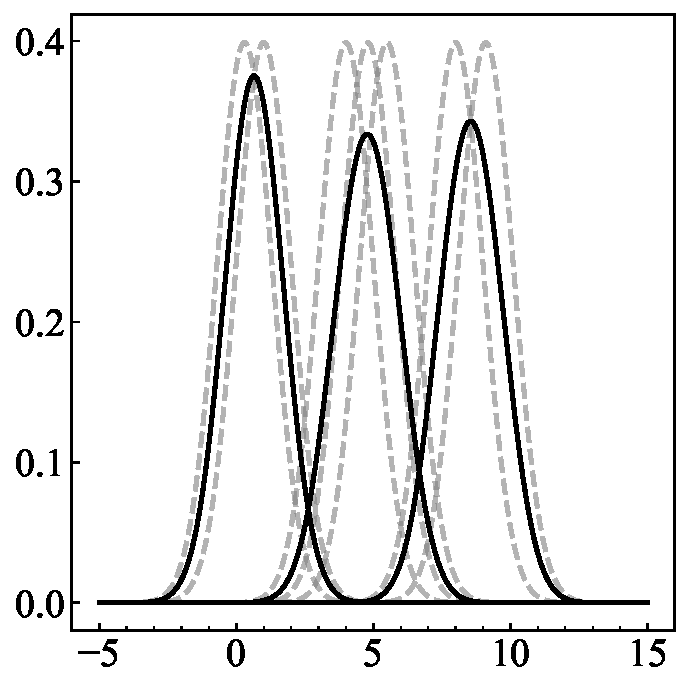
\includegraphics[width=.6\linewidth]{KCF_L2}
			\caption{}
		\end{subfigure}
		\begin{subfigure}[b]{.45\textwidth}
			\centering
			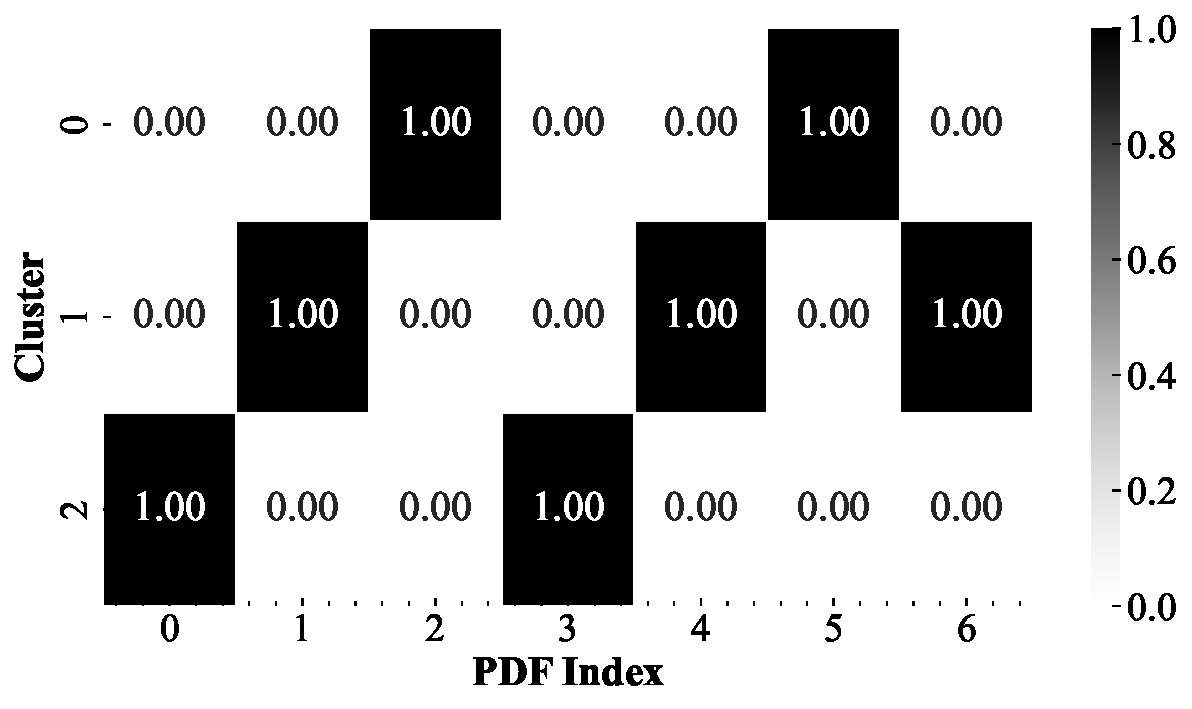
\includegraphics[width=\linewidth]{KCF_U}
			\caption{}
		\end{subfigure}
		\begin{flushleft}
			\footnotesize\it (a) Trọng tâm, và (b) ma trận phân vùng cứng của KCF. Nguồn: Minh họa của tác giả.
		\end{flushleft}
		\caption{Kết quả phân chùm KCF đối với Ví dụ~\ref{vdu:KCF}}\label{figs:vdu:KCF}
	\end{figure}
	
	}


\subsubsection{b.\quad Phân tích chùm thứ bậc (HCF)}

Phân cấp thứ bậc giả định tập $\mathcal{F}^{(t=0)}=\{\{f_1\}\,;\{f_2\}\,;\ldots\,; \{f_n\}\}$ trong \cite{johnson1967hierarchical}  không yêu cầu tiên nghiệm số chùm $c$, mà xây dựng một cây phân cấp bằng cách hợp nhất lần lượt các chùm gần nhất theo một liên kết cho trước. Tại mỗi bước $t=1\,;2\,;\ldots\,;n-1$, ta chọn hai chùm $c_i\,;c_j\in\mathcal{F}^{(t-1)}$ sao cho vị trí $(c_i\,;c_j)=\arg\min_{c_u\,;c_v\in\mathcal{F}^{(t-1)}}\Delta(c_u\,;c_v),$ trong đó, $\Delta(c_u\,;c_v)$ là liên kết giữa hai chùm hàm mật độ. Thuật toán~\ref{alg:HCF} (Phụ lục C, tr.~\pageref{phulucC}) mô tả rõ quy trình thực hiện của phương pháp phân cấp này.

\dly{[Hội tụ của thuật toán HCF]
Giải thuật HCF luôn hội tụ sau $n-1$ bước hợp nhất và tạo thành một cây nhị phân có $n$ nút lá và $n-1$ nút trong.
}
\chm{
	Mỗi lần hợp nhất, một cặp $c_i$, $c_j$ được thay thế bằng chùm $c_i \cup c_j$, và giữ nguyên các chùm còn lại. Ta có 
	$
	\forall  c \in C_t,\; \exists c' \in C_{t+1} \text{ sao cho } c \subseteq c',
	$ tức là $C_{t+1}$ phân rã nhỏ hơn $C_t$.
}


\vdu{[Phân cấp thứ bậc hàm Gauss $1$-chiều]\label{VD:thubac} Ta sử dụng lại dãy hàm mật độ trong Ví dụ~\ref{vdu:KCF}.  Phân cấp thứ bậc với khoảng cách $D(f_1\,;f_2)=\mathcal{L}_2$ và liên kết $\Delta_{\max}(\mathcal{F}_1\,;\mathcal{F}_2)$ là liên kết đủ.

Ta có kết quả phân cấp thứ bậc tích tụ bởi Hình~\ref{figs:thubac} và bài giải chi tiết được phân tích trong Phụ lục B~(tr. \pageref{phulucB}).  Quá trình phân cấp được thực hiện với hai phương pháp liên kết đủ liên kết Ward. Nhìn Hình~\ref{figs:thubac}, ta thấy phương pháp liên kết đủ có xu hướng tạo ra các chùm nhỏ, chặt chẽ, và nhạy cảm với nhiễu ở biên. Ngược lại, liên kết Ward cho kết quả các chùm có tính đồng nhất cao hơn về phân bố, làm cây phân cấp cân đối.

	\begin{figure}[H]
	     \centering
	     \begin{subfigure}[b]{.45\textwidth}
	         \centering
	         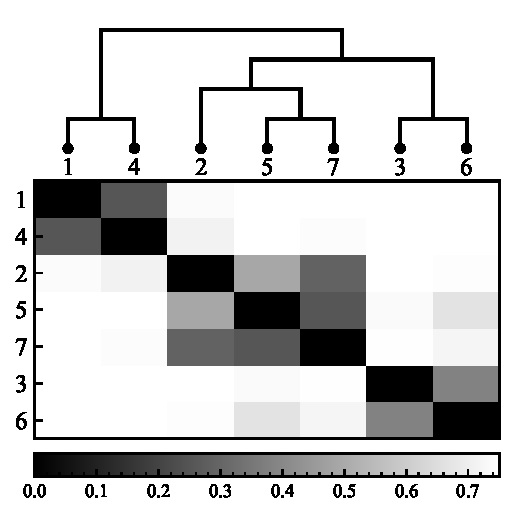
\includegraphics[width=.8\linewidth]{Figs/tree_L2_complete.pdf}
	         \caption{Liên kết đủ}
	     \end{subfigure}
	     \begin{subfigure}[b]{.45\textwidth}
	     	\centering
	     	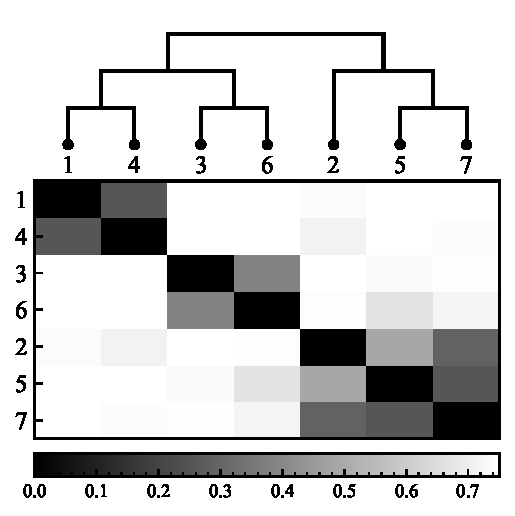
\includegraphics[width=.8\linewidth]{Figs/tree_L2_ward.pdf}
	     	\caption{Liên kết Ward}
	     \end{subfigure}
	     \begin{flushleft}
	     \footnotesize\it Chú thích: Cây phân cấp ở phía trên thể hiện cách sắp xếp và nhóm các hàm mật độ dựa trên liên kết, phần dưới thể hiện ma trận khoảng cách tương ứng với từng hàm mật độ đó. Nguồn: Minh họa của tác giả
	     \end{flushleft}
	     \caption{Kết quả phân cấp thứ bậc tích tụ HCF đối với Ví dụ~\ref{VD:thubac}}\label{figs:thubac}
	\end{figure}
}



%
%\subsubsection{c.\quad Phân tích chùm tự cập nhật}
%
%Phân tích chùm tự cập nhật\index{Phân tích chùm tự cập nhật (Self-Update Process)} (SUP) lần đầu tiên được giới thiệu bởi Chen and Shiu năm 2007 \cite{} với ý tưởng đơn giản là các đối tượng thuộc cùng một chùm sẽ hội tụ tại cùng một điểm. Thuật toán SUP được kết luận khắc phục hiệu quả các vấn đề tồn đọng trong $k$-means, đồng thời chứng minh được sự hội tụ qua các vòng lặp. Sau năm 2015, SUP được phát triển nhanh và nhiều cải tiến mới cho dữ liệu hàm mật độ.
%

\subsection{Phân tích chùm mờ (FCF}

Phân tích chùm mờ được xây dựng lần đầu tiên cho hàm mật độ bởi Thao Nguyen-Trang and Tai Vo-Van \cite{nguyentrang2017fuzzy} với sự phát triển từ phần tử rời rạc do \cite{dunn1973fuzzy}. Khác biệt giữa nó với phân chùm cứng là sự chấp nhận thuộc nhiều chùm của một phần tử với một \emph{mức độ phân vùng} mềm hơn. Điều này hữu ích khi ranh giới giữa các hàm là không chắc chắn.

Giả sử $\mathcal{F}$ chưa được gán nhãn, mục tiêu của bài toán là tối tiểu hóa tổng trọng số các giá trị hàm thành viên với siêu tham số $m$ và khoảng cách.
\begin{align}\tag{FCF}\label{Jf}
	\text{Minimise}\,&:\, J(\bm U\,;\Theta\,|\, \mathcal{F}\,;c\,;m) = \sum_{i=1}^{c}\sum_{j=1}^{n}\mu_{ij}^m{D}^2(\theta_i\,;{f}_j),\\\nonumber
	\text{s.t}\,&:\,\sum_{i=1}^{c} \mu_{ij} = 1,\quad \forall j \in {1, \dots, n}, \tag{C1}\label{c1} \\
	\,&\mu_{ij} \in [0\,;1],\quad \forall i \in {1,\dots,c}, \forall j \in {1,\dots,n}, \tag{C2}\label{c2} \\
	\,&\sum_{j=1}^{n} \mu_{ij} > 0,\quad \forall i \in {1,\dots,c}. \tag{C3}\label{c3}
\end{align}


Thuật toán phân tích chùm mờ cho phần tử rời rạc đã được chứng minh là tối ưu toàn cục bởi \cite{bezdek2013pattern, bezdek1980convergence, hathaway1988recent} qua định lý Zangwill \cite{zangwill1969nonlinear}. Đặc biệt, \cite{groll2005new} mới đây chứng minh sự hội tụ toàn cục qua thuật toán độ dốc\index{độ dốc (gradient method)}. Do đó, luận văn này chỉ giới thiệu Định lý~\ref{thanhlapMU_Theta} trình bày sự thành lập của ma trận phân vùng và hàm mật độ đại diện từ hàm mục tiêu $J$ cho dữ liệu hàm mật độ xác suất.

\dly{\label{thanhlapMU_Theta}Cho $\mathcal{F}$ chứa $n>c$ hàm mật độ xác suất và $m>1$. Xét $D_{ij} = D(\theta_i\,;f_j)$ với $ 1 \le j \le n\,; 1 \le i \le c$. Với mỗi $j$, xác định các tập $I_j = \{i\,|\,D_{ij} = 0, 1 \le i \le c\}$ và tập $I^c_j = \{1\,;\ldots\,;c\} \setminus I_j$. Khi đó $J$ có thể đạt cực tiểu toàn cục khi và chỉ khi
\begin{align}
    \theta^*_i(x)&= \frac{\sum_{j=1}^n(\mu^*_{ij})^mf_j(x)}{\sum_{j=1}^n(\mu^*_{ij})^m}\label{trongtamFCF}\,; \text{ và}\\\label{pvFCF1}
    \mu^*_{ij} &= \frac{(D^*_{ij})^{-1/(m-1)}}{\sum_{l=1}^n(D^*_{lj})^{-1/(m-1)}}\,; \text{ nếu } I_j\ne\emptyset\,;\text{ và},\\\label{pvFCF2}
    \mu^*_{ij} &=0\,;\forall i \in I^c_j \text{ và} \sum_{i\in I^c_j}\mu^*_{ij} =1 \,; \text{ nếu } I_j\ne\emptyset,
\end{align}
}

\chy{
Ở đây, tham số $m$ thể hiện mức độ mờ của ma trận phân vùng $\mu_{ij}$. Khi $m \to 1$, ma trận phân vùng kết quả sẽ tiến về ma trận phân vùng không mờ ($\mu_{ij}=\bm 1_{\{j\in c_i\}}$). Khi $m \to\infty$, các giá trị $\mu_{ij}$ sẽ trở nên bằng nhau ($=1/c$) làm mất khả năng gán các hàm mật độ xác suất vào các chùm. 

Để minh họa ảnh hưởng của tham số $m$, ta giả định hai chùm với $D_{2j}=2-D_{1j}$, và xét giá trị $\mu_{1j}$ theo khoảng cách này chạy từ 0 đến 2. Hình~\ref{fig:phanvung} trực quan hóa cách $m$ điều chỉnh mức độ.  Khi $m\to1$, đường phân vùng trở nên gãy; khi $m$ tăng, đường cong trở nên phẳng và đều ở $y=1/2$.
Nhiều nghiên cứu tổng quát hóa tham số $m$ đã được đặt ra sau khi thuật toán này công bố. Tuy nhiên, cho đến nay các nhà phân tích vẫn chọn tiêu biểu $m=2$ vì tính dễ giải thích \cite{bezdek1980convergence,bezdek1984fcm}. 

\begin{figure}[H]
	\centering
	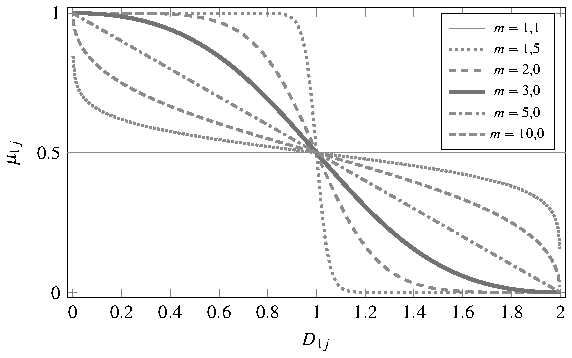
\includegraphics[width=.65\linewidth]{Figs/C1_phanvung.pdf}
	\begin{flushleft}
		\footnotesize \it Chú thích: Giá trị $\mu_{1j}$ tại trục tung biểu diễn mức độ phân vùng tại chùm 1 theo khoảng cách $\bm D_{1j} = \mathcal{L}_1(f_1\,;f_j)$ với các giá trị $m=1{,}1; 1{,}5; 2{,}0; 3{,}0; 5{,}0; 10{,}0$.
		Nguồn: Minh họa của tác giả.
	\end{flushleft}
	\caption{Biểu đồ phân vùng mờ theo khoảng cách $D_{1j}$ với các hệ số $m$ khác nhau.}
	\label{fig:phanvung}
\end{figure}

%Luận văn này, chúng tôi chọn cố định $m=2$.
}

Thuật toán phân chùm mờ FCF được thực hiện qua hai bước cập nhật trọng tâm và cập nhật ma trận phân vùng \citep{nguyentrang2017fuzzy,bezdek1984fcm} (Thuật toán~\ref{alg:FCF}). Kết thúc thuật toán ta nhận được ma trận phân vùng $\bm U_f$ và các trọng tâm chùm $\Theta$. Trong đó, tiêu chuẩn dừng cho FCF là chênh lệch tuyệt đối tối đa giữa các phần tử của ma trận phân vùng ${\bm\mu}^{(t)}$ và ${\bm\mu}^{(t-1)}$ liên tiếp phải thấp hơn ngưỡng dương $\varepsilon$ cho trước. Cuối cùng, ta có thể giải mờ theo quy tắc $c_i = \arg\max_i\mu_{ij}$. Tức là một hàm mật độ $f_j(x)$ được xếp vào chùm $c_i$ khi và chỉ khi nó có mức độ phân vùng tại chùm đó là cao nhất.

\vdu{[Phân chùm mờ hàm Gauss $1$-chiều]\label{VD:FCF} Ta sử dụng lại dãy hàm mật độ trong Ví dụ~\ref{vdu:KCF}. Phân tích $\mathcal{F}$ thành ba chùm, biết $m=2$, tiêu chuẩn dừng $\varepsilon=10^{-3}$, và khoảng cách là $\mathcal{L}_2$. Ta có kết quả sau khi thực hiện các vòng lặp được giải chi tiết ở Phụ lục (tr. \pageref{phulucB}).
	
	
}








\chy{
	Dựa vào giá trị phân vùng $\mu_{ij}$, ta nhận thấy được mức độ tin cậy một hàm mật độ $f_j(x)$ xếp vào chùm $c_i$. Nếu giá trị phân vùng $\mu_{ij}$ tại chùm $c_i$ này lớn, ta có thể chắc chắn vào kết quả phân bổ, ngược lại, nếu giá trị này không cao, ta biết được hàm mật độ này có khả năng thuộc vào một chùm khác hoặc một chùm mới thay vì thuộc vào chùm $c_i$.
	}


So sánh về mặt phức tạp thời gian và phức tạp dung lượng, Bảng~\ref{C1:Complexity} cho thấy phương pháp $k$-mean đơn giản hơn và ít tốn tài nguyên tính toán hơn so với Fuzzy $c$-mean và thuật toán thứ bậc. 
	
\begin{table}[H]
	\centering
	\footnotesize
	\caption{So sánh độ phức tạp của ba thuật toán phân chùm}\label{C1:Complexity}
	\begin{tabular*}{\columnwidth}{@{\extracolsep\fill}lll@{\extracolsep\fill}} 
		\toprule
		\bf Thuật toán               & \bf Phức tạp thời gian              & \bf Phức tạp không gian \\ 
		\midrule
		Phân chùm KCF                    & $\mathcal{O}(n c d i)$              & $\mathcal{O}(n + c d)$    \\
		Phân cấp HCF          & $\mathcal{O}(n^2 \log n)$           & $\mathcal{O}(n^2)$        \\
		Phân chùm FCF             & $\mathcal{O}(n c d i)$              & $\mathcal{O}(n c)$    \\
		\bottomrule
	\end{tabular*}
	\begin{flushleft}\footnotesize
	\textit{Chú thích}: $n$ là \# đối tượng trong dữ liệu, $c$ là \# chùm, $d$ là \# chiều dữ liệu, $i$ là \# vòng lặp.
	\end{flushleft}
	
\end{table}



\section{Phân loại cho hàm mật độ xác suất}
Ở dữ liệu rời rạc, bốn thuật toán phân loại kinh điển dựa vào thống kê là Naive Bayes, Cây quyết định, hồi quy Logistics, phân biệt Fisher \cite{fisher1936use} và Perceptron \cite{rosenblatt1961principles} đã được áp dụng phát triển cho đến hiện nay. Trong khi đó, các phát triển phân loại hàm mật độ chỉ dựa trên phương pháp Bayesv. Luận văn này tập trung nghiên cứu phương pháp hồi quy logistics, máy véc-tơ hỗ trợ\index{máy véc-tơ hỗ trợ (support vector machine)}, và đặc biệt là phương pháp Bayes cho dữ liệu hàm mật độ \cite{huynh2024classifying,vo2024supervised}. 
\subsection{Hồi quy logistics}

Phương pháp này được tổng quát hóa cho dữ liệu hàm bởi các nghiên cứu của Akturk et al. \cite{akturk2024robust}. Luận văn này cụ thể hóa cho hàm mật độ xác suất. Mô hình hồi quy logistic cho dữ liệu hàm mật độ có dạng
\begin{align}\label{eq:log} \pi _j = {\mathbb {P}}(Y_j = 1 \vert f(x) = f_j(x)) =  \frac{\exp \left\{ \beta _0 + \int _{\Omega} f(x) \beta (x) \mathrm{\,d}x \right\} }{1 + \exp \left\{ \beta _0 + \int _{\Omega} f(x) \beta (x) \mathrm{\,d}x \right\} }, \end{align}
trong đó $\beta_0\in \mathbb{R}$ là hằng số chặn\index{hằng số chặn (intercept)}, và $\beta(x) \in\mathcal{L}_2[\Omega]$ là hàm hệ số\index{hàm hệ số $\beta(x)$ ($\beta$-functional coefficient)} cần ước lượng. Để giải phương trình~\eqref{eq:log}, biến đổi logit được sử dụng
$$
\ell_j = \log\left(\frac{\pi_j}{1-\pi_j}\right) = \beta_0 + \int _{\Omega} f(x) \beta (x) \mathrm{\,d}x.
$$


Mục tiêu tiếp theo là ước lượng $\beta_0$ và hàm $\beta(x)$. Do $\beta(x)$ là vô hạn chiều, ta chiếu hàm này vào một tập hàm cơ sở\index{hàm cơ sở (basis functions)} chọn trước để ước lượng, cụ thể là hàm Gauss, wavelet, chuỗi Fourier, đa thức Bernstein và Legendre, hoặc B-spline (Xem thêm Bảng~\ref{tab:basis_functions} tại Phụ lục C, tr.~\pageref{phulucC}). Khi đó,
$$
\ell_j = \beta_0 + \sum_{m=1}^M \theta_m \underbrace{\int_\Omega \psi_m(x) f_i(x)\, dx}_{=: \bm\Phi=\phi_{j,m}},
$$
trong đó $\phi_{j,m}$ là mô-men của hàm mật độ $f_j(x)$ trên hàm cơ sở $\psi_m(x)$. 



Bài toán ước lượng $\beta(x)$ chuyển thành cực đại hóa log-likelihood của hồi quy logistics
$$
\ell(\beta_0\,;\beta(x))= \max_{\substack{\beta_0\in\mathbb{R},\\\beta(x)\in\mathbb{R}^M}}\left\{\underbrace{\sum_{j=1}^n \left[y_j \log \pi_j + (1 - y_j)\log (1 - \pi_j)\right]}_{Logistics} - \underbrace{\lambda_1\sum_{m=1}^M\vert\beta_m(x)\vert }_{Lasso} \underbrace{-\frac{\lambda_2}{2}\sum_{m=1}^M\beta_m(x)^2}_{Ridge}\right\},
$$ 
trong đó, $\pi _j = {\mathbb {P}}(Y_j = 1 \vert f(x))$ và $\ell$ là hàm mất mát\index{hàm mất mát (loss function)}.

\begin{theorem}\label{dly:loi}
	Hàm mất mát $\ell$ là một hàm lồi theo cả $\beta_0$ và $\beta(x)$. Nếu $\lambda_2 > 0$ thì hàm này lồi nghiêm ngặt. Vì vậy, nghiệm tối ưu toàn cục luôn tồn tại duy nhất.
\end{theorem}

Từ Định lý~\ref{dly:loi}, ta tính được Gradient theo hệ số $\beta(x)$ với $\hat{y}_j = \pi_j$ là xác suất dự đoán, có dạng
	$
	\nabla_{\bm\beta} \ell = \Phi^\intercal (y - \hat{y}) - \lambda_1 \,\text{sign}(\beta(x)) - \lambda_2 \beta,
	$
mà qua đó ta có nhiều phương pháp tối ưu như tối ưu độ dốc như ADAM, hay các quasi-Newton khác như L-BFG-S.



\vdu{[Phân loại hàm mật độ bằng hồi quy logistic]\label{VD:log}
	Xét hai lớp hàm mật độ Gauss $\mathcal{F}$ và $\mathcal{G}$ với các trung tâm lần lượt là
	$
	\mu_\mathcal{F}=\{1,0;\,1,5;\,2,0;\,2,5;\,6,0\}$,  và $
	\mu_\mathcal{G}=\{4,5;\,7,5;\,8,5;\,8,0;\,9,0\},	$
	trong đó phương sai lần lượt là $\sigma_{\mathcal{F}}^2 = 0,4$ và $\sigma_{\mathcal{G}}^2 = 0,9$.
	Bài toán đặt ra là phân loại một hàm mật độ Gauss mới
	$
	h(x) = \mathcal{N}(3,0; 0,9)
	$
	vào một trong hai lớp $\mathcal{F}$ hoặc $\mathcal{G}$.
	
	Sử dụng $M=10$ hàm cơ sở Gauss, ta ước lượng được hàm hệ số $\widehat{\beta}(x)$, phản ánh đóng góp của từng miền $x$ đối với phân loại. Hàm $\widehat{\beta}(x)$ được tái tạo và minh hoạ ở Hình~\ref{fig:beta_log}.
	
	\begin{figure}[H]
		\centering
		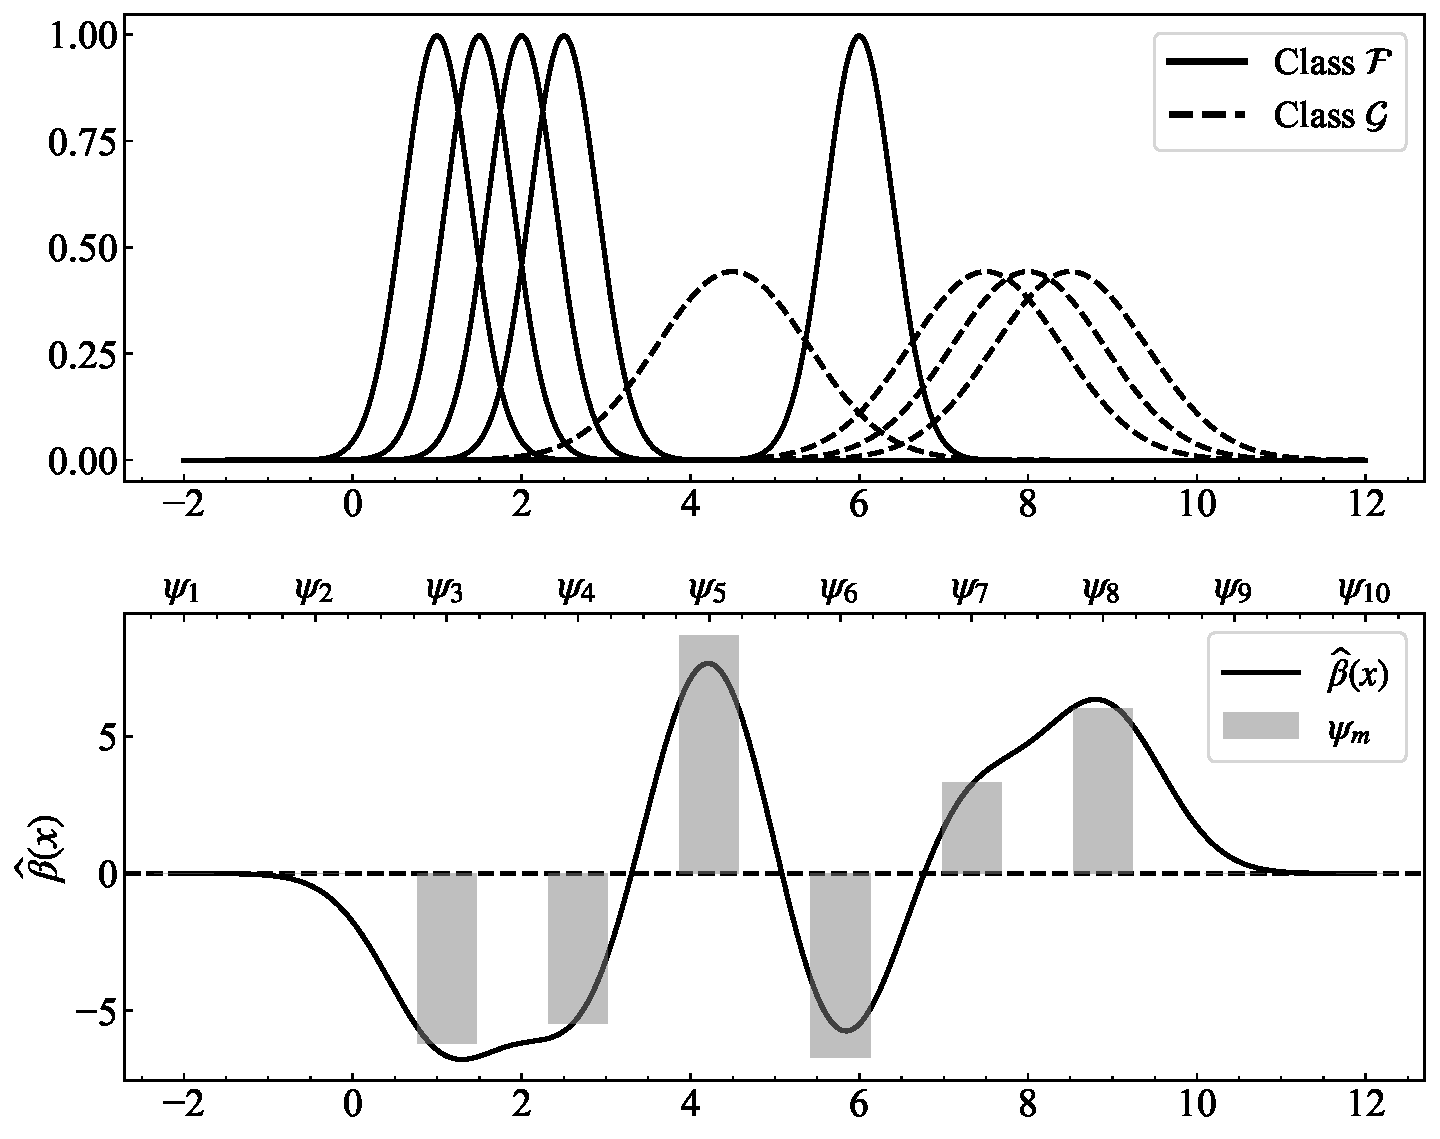
\includegraphics[width=0.7\linewidth]{Figs/C1_beta_log}
		\caption{Hàm $\widehat\beta(x)$ được ước lượng qua $10$ hàm cơ sở Gauss.}
		\label{fig:beta_log}
	\end{figure}
	
Tiếp theo, để phân loại $h$, ta cũng chiếu lên không gian cơ sở. Hàm $h$ được chiếu lên $10$ hàm cơ sở Gauss để tạo thành véc-tơ đặc trưng được đưa vào mô hình logistic đã huấn luyện. Cuối cùng, mô hình logistic dự đoán xác suất $h$ thuộc lớp $\mathcal{F}$ là $43{,}26\%$. Do đó, ta phân loại $h(x)$ vào lớp $\mathcal{F}$.
	
}


\chy{
	Hàm hệ số $\widehat{\beta}(x)$ đóng vai trò như một công cụ giải thích quan trọng, cho phép đánh giá mức độ đóng góp của từng miền $x \in \Omega$ đối với quá trình phân loại nhị phân. Đáng chú ý, $\widehat{\beta}(x)$ cung cấp một dạng giải thích bằng tính năng, giúp ta hiểu thêm nguồn gốc của từng đóng góp riêng lẻ đến xác suất phân loại.
}

Hình~\ref{fig:beta_log} cho thấy $\widehat{\beta}(x)$ dao động quanh trục $0$ với cả miền dương và âm, phản ánh rằng các vùng khác nhau của $x$ có ảnh hưởng trái ngược đến xác suất dự đoán. Những vùng mà $\widehat\beta(x) > 0$ sẽ tăng xác suất dự đoán lớp $1$, và ngược lại. Cụ thể, các hệ số $\psi_5$ và $\psi_8$ có giá trị dương thể hiện tác động tăng xác suất dự đoán, trong khi $\psi_3$ và $\psi_6$ mang giá trị âm, góp phần làm giảm xác suất của lớp $\mathcal{F}$. Việc áp dụng các kỹ thuật chuẩn hoá Ridge làm giảm hệ số một cách đồng đều, còn Lasso tạo ra sự chọn lọc hàm cơ sở $\psi_m$ quan trọng.



\subsection{Máy véc-tơ hỗ trợ}



Cho tập huấn luyện
$
\mathcal{D} = \{(f_j, y_j)\}_{j=1}^n\,; f_j \in \mathcal{F},\; y_j \in \{-1, 1\}.
$ Bài toán máy véc-tơ hỗ trợ lề mềm được xây dựng từ nguyên lý cực tiểu hoá độ lớn véc-tơ trọng số $\bm{w}$ và cho phép sai số điều chỉnh được bởi các biến $\xi_j$, tức là
\begin{align*}
	\text{Maximise} & \;: \frac{1}{2} \|\bm{w}\|_{\mathcal{H}}^2 + C \sum_{j=1}^n \xi_j, \\
	\text{S.t.} & \;: y_j \left( \langle \bm{w}, \Phi(f_j) \rangle + b \right) \ge 1 - \xi_j, \\
	&\quad \xi_j \ge 0, \quad j = 1, \dots, n.
\end{align*}

Hàm L'Agrange tương ứng được cho bởi
\[
\mathcal{L}(\bm{w}, b, \bm{\xi}, \bm{\alpha}, \bm{\mu}) =
\frac{1}{2} \|\bm{w}\|^2 + C \sum_{j=1}^n \xi_j 
- \sum_{j=1}^n \alpha_j \left[y_j \left(\langle \bm{w}, \Phi(f_j) \rangle + b \right) - (1 - \xi_j) \right] 
- \sum_{j=1}^n \mu_j \xi_j.
\]


Lấy đạo hàm theo $\bm{w}$ và đặt $\nabla_{\bm{w}} \mathcal{L} = 0$. ta có $
\bm{w} = \sum_{j=1}^n \alpha_j y_j \Phi(f_j)$. Thay vào hàm  L'Agrange, ta được bài toán đối ngẫu của SVM được định nghĩa bởi
\begin{align}\tag{SVM}\label{eq:svm-dual}
	\text{Maximise} & \;: \sum_{j=1}^n \alpha_j 
	- \frac{1}{2} \sum_{j=1}^n \sum_{k=1}^n \alpha_j \alpha_k y_j y_k \underbrace{\langle \Phi(f_j), \Phi(f_k) \rangle}_{K(f_j, f_k)}, \\
	\text{S.t.} & \;: 0 \le \alpha_j \le C,\quad \sum_{j=1}^n \alpha_j y_j = 0.
\end{align}

\dly{\ref{eq:svm-dual} là bài toán tối ưu lồi nghiêm ngặt trên đa diện lồi compact, do đó tồn tại duy nhất nghiệm véc-tơ \(\boldsymbol{\alpha}^{*}\in\mathbb{R}^{n}\).}


\chm{Ma trận Gram $\bm{G}_{jk} = y_j y_k K(f_j, f_k)$ là xác định dương do $K$ là kernel thỏa mãn điều kiện Mercer. Hàm mục tiêu là hiệu của một hàm tuyến tính và một dạng toàn phương xác định dương nên lồi nghiêm ngặt. Nhờ đó, tồn tại nghiệm cực đại duy nhất theo định lý Weierstrass.}

%\begin{theorem}[Điều kiện KKT cho máy véc-tơ hỗ trợ lề mềm]
%	Với mọi $j = 1,\dots,n$, nghiệm $(\bm{\alpha}^*, \bm{\xi}^*, \bm{\mu}^*)$ thoả điều kiện KKT bao gồm
%	\begin{enumerate}
%		\item \(\alpha_j \left[ y_j\, g(f_j) - (1 - \xi_j) \right] = 0,\) với \(g(f_j) = \sum_{k=1}^n \alpha_k y_k K(f_k, f_j) + b,\)
%		\item \(\mu_j\, \xi_j = 0,\)
%		\item \(\alpha_j + \mu_j = C.\)
%	\end{enumerate}
%\end{theorem}

\dly{Tại nghiệm $\bm{\alpha}^*$, khoảng cách đến siêu phẳng tối ưu là
	$$
	\rho =\frac{1}{\lVert\bm w\rVert} =\left( \sum_{j=1}^n \sum_{k=1}^n \alpha_j^* \alpha_k^* y_j y_k K(f_j, f_k) \right)^{-1/2}.
	$$
	Khi đó, hàm phân lớp tương ứng đối với hàm mật độ mới $h$ là
	\[
	\hat{y}(h) = \operatorname{sign}\!\left( g(h) \right) = 
	\operatorname{sign}\!\left( \sum_{j=1}^n \alpha_j^* y_j K(f_j, h) + b^* \right).
	\]
}









\subsection{Phương pháp naive Bayes}


\subsubsection{a\qquad Thuật toán phân lớp}

Phương pháp naive Bayes đã được nhiều nhà thống kê quan tâm cho dữ liệu hàm mật độ xác suất bởi \cite{ren2009naive}. 
Cho tập huấn luyện
$
\mathcal{D} = \{(f_j, y_j)\}_{j=1}^n\,; f_j \in \mathcal{F},\; y_j \in \{0, 1\}.
$
Xác suất hậu nghiệm Bayes để xếp $h(x)$ vào lớp $Y=k$ được viết dưới dạng
\begin{equation}
	\mathbb{P}(Y=k\,|\,h) \;=\; 
	\frac{\mathbb{P}(Y=k)\, f(h\,|\,Y=k)}
	{\sum_{j\in\{0,1\}} \mathbb{P}(Y=j)\, f(h \,|\,Y=j)}.
\end{equation}

Khi này, ta ước lượng mật độ có điều kiện $f(h \,|\, Y=k)$ bằng kỳ vọng của hàm hạt nhân giữa đối tượng mới $h$ và các hàm mật độ huấn luyện $f_i$ trong lớp $Y=k$. Tức là,
\begin{align}
	f(h \,|\, Y=k) 
	= \frac{1}{n_k bw_k} \sum_{i=1}^{N_k} 
	\mathbb{E}_{X \sim h,\; Y \sim f_{i}}
	\!\left(
	\kappa\!\left(\frac{X-Y}{bw_k}\right)
	\right), \label{eq:kernelbayes}
\end{align}
trong đó $n_k$ là số mẫu huấn luyện thuộc lớp $Y=k$, 
$f_i$ là các hàm mật độ huấn luyện trong lớp đó, 
và $bw_k$ là tham số trơn.
Dưới dạng tích phân, công thức \eqref{eq:kernelbayes} tương đương với
$$
	f(h \,|\, Y=k) 
	= \frac{1}{n_k}\sum_{i=1}^{n_k} 
	\iint \frac{1}{bw_k}\, \kappa\left(\frac{x-y}{bw_k}\right)\, h(x)\, f_{i}(y)\, \mathrm{d}x\, \mathrm{d}y.
$$

Giả sử không có thông tin tiên nghiệm, ta lấy tiên nghiệm đều $\mathbb{P}(Y=1) = \mathbb{P}(Y=0) = 1/2$. Khi này ta có quy tắc phân loại hàm mật độ $h(x)$ phân loại vào lớp $Y=1$ nếu $
f(h\,|\, Y=1) > f(h \,|\, Y=0)$ và ngược lại. Tương tự, đối với phân loại nhiều hơn hai lớp, hàm mật độ $h$ sẽ được phân loại vào lớp $k$ nào có hậu nghiệm lớn nhất, tức là $$
\widehat{y}=\arg\max_{k\in\{1\,;\ldots\,;K\}} \mathbb{P}(Y=k \,|\, h).$$

\bode{[Hàm mật độ Gauss có điều kiện] \label{bde:kernel-gauss}
	Xét công thức ước lượng mật độ có điều kiện $
	f(h \,|\, Y=k)$. Nếu chọn hạt nhân Gauss 
	$\kappa(u) = \mathcal{N}(u;0,1)$, thì ta có
	\[
	f(h \,|\, Y=k)
	=\frac{1}{n_k}\sum_{i=1}^{n_k} 
	\mathcal{N}\!\Big(\mu_h-\mu_i;\,0,\,\sigma_h^2+\sigma_i^2+bw_k^2\Big),
	\]
	trong đó $\mathcal{N}(\cdot;0,\tau^2)$ là mật độ Gauss với trung bình $0$ và phương sai $\tau^2$.
}

\chm{
	Ta có 	$\kappa\left(\frac{x-y}{bw_k}\right) = \mathcal{N}(x-y;0,bw^2_k)$. Ngoài ra, viết lại tích phân đôi theo biến $z=x-y$, ta có
	$$
	\iint \mathcal{N}(z;0,bw_k^2)\,h(y+z)\,f_i(y)\,\mathrm{d}z\,\mathrm{d}y.
	$$
	Đặt $X\sim\mathcal N(\mu_h,\sigma_h^2)$ và $Y\sim\mathcal N(\mu_i,\sigma_i^2)$ độc lập. 
	Khi đó biến ngẫu nhiên $Z=X-Y$ cũng tuân theo phân phối chuẩn (Bổ đề~\ref{ble:sum-Gauss}), tức là
	$
	Z \sim \mathcal N(\mu_h-\mu_i,\ \sigma_h^2+\sigma_i^2).
	$
	Do đó, giá trị $f(h \,|\, Y=k)$ có thể viết thành kỳ vọng
	$$
	f(h \,|\, Y=k)
	=\int \mathcal{N}(z;0,bw_k^2)\,\mathcal{N}\big(z;\mu_h-\mu_i,\sigma_h^2+\sigma_i^2\big)\,\mathrm{d}z.
	$$
	
	Áp dụng Bổ đề~\ref{ble:tich-Gauss} về tích phân của tích hai mật độ chuẩn 
	với $a=bw_k^2$, $b=\sigma_h^2+\sigma_i^2$, $m=\mu_h-\mu_i$ ta thu được điều phải chứng minh.
}


\vdu{[Phân loại hàm mật độ bằng phương pháp naive Bayes]
	Trở lại giả thuyết của Ví dụ~\ref{VD:log}, ta cần phân loại hàm mật độ Gauss mới 
	$h(x)=\mathcal{N}(3{,}0;\,0{,}9)$ vào một trong hai lớp.
	
	\textbf{Bài giải.} Giả sử không có thông tin tiên nghiệm, 
	$\mathbb{P}(Y{=}1)=\mathbb{P}(Y{=}0)=0{,}5$. Theo Bổ đề~\ref{bde:kernel-gauss} ta có
	$$
	f(h\,|\,Y=k)
	=\frac{1}{n_k}\sum_{i=1}^{n_k}
	\frac{1}{\sqrt{2\pi\big(\sigma_h^2+\sigma_{i}^2+bw_k^2\big)}}
	\exp\!\left(
	-\frac{(\mu_h-\mu_{i})^2}{2\big(\sigma_h^2+\sigma_{i}^2+bw_k^2\big)}
	\right).
	$$
		
Dùng quy tắc Silverman cho từng lớp, ta có
$$
	h_{\mathcal{F}}
	=1{,}06\,\sqrt{0{,}4}\,(n_\mathcal{F})^{-1/5}= 0{,}486, \text{ và }
	h_{\mathcal{G}}
	=1{,}06\,\sqrt{0{,}9}\,(n_\mathcal{G})^{-1/5}= 0{,}729,
$$
	Khi này, ta tính được $f(h\,|\,\mathcal{F})$ qua các kỳ vọng $\mu_\mathcal{F}$, ta có kết quả
$
		f(h\,|\,\mathcal{F})= 0{,}158.
$
Tương tự, ta cũng tính được $f(h\,|\,\mathcal{G})$ qua với các kỳ vọng $\mu_\mathcal{F}$, kết quả là
$
		f(h\,|\,\mathcal{G}) = 0{,}033.
$
	
Cuối cùng, xác suất hậu nghiệm của hai lớp được tính bởi công thức
	\[
	\mathbb{P}(\mathcal{F}\,|\,h)=
	\frac{0{,}5\,f(h\,|\,\mathcal{F})}{0{,}5\,f(h\,|\,\mathcal{F})+0{,}5\,f(h\,|\,\mathcal{G})}
	=
	\frac{0{,}5\cdot 0{,}158}{0{,}5\cdot 0{,}158+0{,}5\cdot 0{,}033}
	= 0{,}826,
	\]
	và $\mathbb{P}(\mathcal{G}\,|\,h)=1-0{,}826=0{,}174$. 
	Vì $\mathbb{P}(\mathcal{F}\,|\,h)>\mathbb{P}(\mathcal{G}\,|\,h)$ 
	nên $h(x)$ được phân loại vào lớp $\mathcal{F}$ với xác suất hậu nghiệm xấp xỉ $82{,}6\%$.

}



\subsubsection{b\qquad Xác định tiên nghiệm}
Trong bài toán phân loại Bayes, xác suất tiên nghiệm $\mathbb{P}(Y=k)$ thường được ước lượng bằng nhiều cách khác nhau, thông thường là dựa vào kiến thức chuyên gia hoặc thông tin trong lịch sử nghiên cứu tương tự hoặc dữ liệu lớn. Trong trường hợp không có thông tin tiên nghiệm nào, ta có thể giả định mọi lớp đều có xác suất bằng nhau, tức là $\mathbb{P}(Y=k)=1/k$. Trong nhiều tình huống, xác suất tiên nghiệm còn có thể ước lượng từ tần suất xuất hiện của các lớp trong tập dữ liệu huấn luyện. Khi đó, $\mathbb{P}(Y=k)=n_k/n$  trong đó $n_k$ là số lượng mẫu thuộc lớp $k$ và $n$ là tổng số mẫu. Tuy nhiên, phương pháp này có thể gặp vấn đề khi dữ liệu ít hoặc có xác suất bằng $0$ cho một số lớp, phương pháp Laplace được sử dụng để điều chỉnh, $\mathbb{P}(Y=k) = (n_k+\alpha)/(n+\alpha k)$, trong đó $\alpha>0$.





\section*{Tổng kết Chương \ref{chapter_1}}
\addcontentsline{toc}{section}{Tổng kết chương \ref{chapter_1}}

Chương \ref{chapter_1} trình bày cơ sở lý thuyết của hàm mật độ xác suất, các phép đo khoảng cách và phương pháp phân tích chùm/phân loại. Những kiến thức này đóng vai trò nền tảng cho các chương tiếp theo.
















%
\chapter{NHẬN DẠNG THỐNG KÊ CHO HÀM MẬT ĐỘ XÁC SUẤT\\VỚI~DỮ~LIỆU MẤT~CÂN~BẰNG}\label{chapter_2}

\section{Giới thiệu}



Hàm mật độ xác suất được xem là dạng dữ liệu đặc trưng\index{dữ liệu đặc trưng (symbolic data)} với cấu trúc phức tạp hơn. Nó cho phép khám phá quy luật phân bố tại nhiều tổng thể khác nhau hoặc được xem như đối tượng không chắc chắn khi quyết định chưa chính xác hoặc có lỗi.

Trong dữ liệu $1$-chiều, nghiên cứu về Cá hồi vây vàng (\textit{Yellowfin tuna}) của Minami \cite{minami2024regression} thể hiện phân bố chiều dài cá theo từng ô tọa độ tại Thái Bình Dương. Bên cạnh đó, các phân phối liên quan đến phân phối tỷ giá theo ngày, khí hậu ở các trạm theo năm, hay mật độ tuổi giữa hai giới ở các tỉnh, chỉ số sức khỏe theo độ tuổi \cite{irpino2015basic,billard2012symbolic} cũng là ví dụ tiêu biểu cho dạng $1$-chiều. Đặc biệt, dữ liệu hàm mật độ còn có thể được xây dựng từ hình ảnh thông qua việc trích xuất màu sắc \cite{nguyen2024new,vo2024supervised}. Trong khi đó, dữ liệu $2$-chiều thường xuất hiện trong các nghiên cứu về mối tương quan, ví dụ phân tích điểm số sinh viên giữa các khoa/viện tại Đại học Cần Thơ \cite{vovan2019cluster}. Hoặc là sự mở rộng ảnh hưởng từ các véc-tơ rời rạc đa chiều \cite{tavakkol2021fuzzy}.

Tuy nhiên, quá trình thu thập dữ liệu này thường mất nhiều thời gian, và khó khăn trong lưu trữ và không gian vô hạn chiều. Cho nên, nhiều phương pháp tiếp cận mới từ nhận dạng thống kê đã giải quyết nhu cầu phân tích dạng dữ liệu này. Chúng bao gồm phân tích chùm và phân loại hàm mật độ xác suất. 


%
%
%Phần này sử dụng ánh xạ đo được $\mathcal{F}\,:\,(\Omega, \mathcal{S}, P) \to (\mathcal{D}\,,\mathcal{B}_D)$ với $(\Omega, \mathcal{S}, P)$ là không gian xác suất và  sigma-đại số Borel $\mathcal{B}_D$  trên $(\mathcal{D}, d)$. Một tập đối tượng hàm mật độ quan sát là $f_j\sim\mathcal{F}$ với $j=1\,,\ldots\,,n$ (Định nghĩa~\ref{dng:data1} và \ref{dng:datad}).
%
%\dng{[Hàm đại diện Fréchet]\label{dng:frechet}
%	Phần tử hàm đại diện $f^* \in \mathcal{D}$ sao cho
%	\begin{align}
%		\theta=\arg\min_{g \in \mathcal{D}} \; \mathbb{E}\!\left(D^2\big(\mathcal{F},g\big)\right),
%		\label{eq:frechet_mean}
%	\end{align} là hàm đại diện Fréchet.
%}




\subsection{Phương pháp phân tích chùm hàm mật độ xác suất}


Phân tích chùm là một nhánh chính của nhận dạng không được giám sát \cite{jain2010data,saxena2017review,dinh2025categorical}. Nó có nhiệm vụ khám phá dựa vào sự tương tự giữa các mẫu trong dữ liệu đầu vào \cite{Bishop:DeepLearning24,webb2003statistical}. Ví dụ như khi ta cần khoanh vùng khối u trong hình ảnh MRI,  hay trong các báo cáo định tính cần nhóm/tổng hợp ý kiến hay quan điểm theo các chủ đề khác nhau.   Đầu ra của phân tích chùm là các nhãn cho dữ liệu ban đầu. 
%Nhiều họ các phân chùm có cách phân chia khác nhau, nhưng mục tiêu chung là sự phân bổ tối tiểu khoảng cách phần tử trong chùm trong khi vẫn giữ tối đa khoảng cách phần tử giữa các chùm. 
% Ta cũng có phân tích chùm các hàm mật độ xác suất là bài toán phân tích chùm cho đối tượng các hàm mật độ xác suất  
%Các thuật toán này được chia thành hai loại dựa theo lý thuyết mờ \cite{bezdek2013pattern} là phân chùm không mờ (bao gồm KCF \cite{nguyen2024new}, HCF , và SUP), và phân chùm mờ (bao gồn FCF \cite{nguyentrang2017fuzzy,vovan2019cluster}). 



Bảng~\ref{tab:in_clustering_summary} mô tả quá trình phát triển phương pháp phân tích chùm hàm mật độ giai đoạn 5 năm từ 2019 đến 2024. Nhìn chung, các nghiên cứu cho thấy sự phát triển cả về bề sâu và bề rộng. Các hàm mục tiêu SSE và VCC dần được mở rộng và phức tạp hơn, như CSB và FSF cho phép đánh giá chất lượng của kết quả phân tích chùm một cách đa chiều và sâu sắc hơn. Nghiên cứu của Thao Nguyen-Trang đã sử dụng FSF \cite{nguyen2023globally}, hoặc CSB \cite{nguyen2023balance} làm mục tiêu phân chùm, cho thấy nghiên cứu đã đào sâu vào nội hàm thuật toán. Hơn nữa, năm 2019 cho thấy sự mở rộng từ mô hình cứng sang các phương pháp khác như mờ, khả dĩ và bán giám sát. Các nghiên cứu giai đoạn 2019 tập trung vào các mô hình phân chùm cứng, như $k$-medoids, KCF. Từ năm 2019 trở đi, các nghiên cứu đã bắt đầu chuyển sang sử dụng các mô hình phân chùm mờ, như trong Tai Vo-Van \cite{vovan2019cluster, phamtoan2022automatic}, đã sử dụng FCF với $m=2$.  Cuối năm 2024, nhóm tác giả Thao Nguyen-Trang \cite{nguyen2024new} đã giới thiệu một mô hình phân chùm bán giám sát, sử dụng một phần dữ liệu có nhãn để cải thiện kết quả phân chùm. 

\begin{table}[H]
	\centering
	\scriptsize
	\begin{tabular*}{\textwidth}{@{\extracolsep\fill}lp{4cm}p{6cm}lp{1.5cm}@{\extracolsep\fill}} 
		\toprule
		\textbf{Năm} & \textbf{Tác giả} & \textbf{Mô tả phương pháp} & \textbf{Khoảng cách} & \textbf{Phân chùm tự động} \\
		\midrule
		2019 & Tai Vo-Van \cite{vovan2019cluster} & Phân chùm FCF, $m=2$, tìm số chùm bằng SUP & Độ rộng chùm & $\times$ \\
		2019 & Dinh Pham-Toan \textit{et al.} \cite{pham2019new} & Phân chùm $k$-medoids, tối tiểu SSE bằng nhị phân aeDE, số chùm cho trước & $\mathcal{L}_2$ & $\times$   \\
		2020 & Dinh Pham-Toan \& Tai Vo-Van \cite{phamtoan2022automatic}& Phân chùm FCF, tối tiểu VCC bằng nhị phân GA, $m=2$, tìm số chùm bằng SUP   & $\mathcal{L}_1$ &  $\times$ \\
		2023 & Thao Nguyen-Trang, Tai Vo-Van  \& Ha Che-Ngoc \cite{nguyen2024efficient} & Phân chùm tự cập nhật cải tiến, tự động dựa trên SUP &  hạt nhân Gauss $\mathcal{L}_1$ & $\times$ \\
		2023 & Thao Nguyen-Trang \textit{et al.} \cite{nguyen2023balance} & Phân chùm cứng, tối tiểu CSB bằng DE, hàm đại diện Gauss  & $\mathcal{L}_2$ & $\checkmark$ \\
		2023 & Thao Nguyen-Trang, Trung Nguyen-Thoi, \& Tai Vo-Van \cite{nguyen2023globally} & Phân chùm FCF, tối tiểu FSF bằng DE, hàm đại diện Gauss, $m=1$ & $\mathcal{L}_1$ & $\checkmark$ \\
		2024 & Hung Tran-Nam, Thao Nguyen-Trang \& Ha Che-Ngoc \cite{tran2024new} & Phân chùm khả dĩ, tối tiểu SSE, chọn ngưỡng bất thường bằng $\alpha$-cut, $m=2$, số chùm cho trước  & $\mathcal{L}_2$ &  $\times$\\
		2024 &Thao Nguyen-Trang, Yen Nguyen-Hoang \& Tai Vo-Van \cite{nguyen2024new} & Phân chùm KCF, tối tiểu SSE, bán giám sát bằng \% nhãn cho trước, số chùm cho trước & $\mathcal{L}_1$ & $\times$ \\
		\bottomrule
	\end{tabular*}
	\begin{flushleft}\it\footnotesize
		Đối với hàm mục tiêu, SSE: sai số của bình phương tối tiểu; VCC: tiêu chuẩn tỷ lệ phương sai (chỉ số Calinski--Harabasz); CSB: hợp của độ đo tương đồng và cân bằng; FSF: tỷ lệ giữa SSE và sự phân biệt giữa các chùm. Đối với phương pháp tối ưu, DE:  tiến hóa vi phân; aeDE: tiến hóa vi phân ưu tú thích nghi; GA: giải thuật di truyền. Ở cột cuối, dấu $\checkmark$ có nghĩa là tự động toàn bộ thuật toán.
	\end{flushleft}
	\caption{Tổng quan giai đoạn 5 năm (2019--2024) nghiên cứu phân tích chùm cho hàm mật độ xác suất}
	\label{tab:in_clustering_summary}
\end{table}


Ở quốc tế, hai công trình tiêu biểu thể hiện hai hướng tiếp cận khác nhau. Chen \& Hung (2020) \cite{chen2021jackknife} nhấn mạnh vào tiêu chuẩn thông tin để tự động phát hiện cấu trúc chùm và xác định số chùm tối ưu, trong khi Tavakkol \& Son (2021) \cite{tavakkol2021fuzzy} tập trung vào không gian hạt nhân để xử lý các chùm có hình dạng bất quy tắc. Điểm chung là cả hai đều mở rộng nền tảng của phân chùm truyền thống. Về ứng dụng, giải thuật entropy-jackknife là phân chùm cứng cho dữ liệu hình ảnh, trong khi Tavakkol \& Son thích hợp cho dữ liệu hàm mật độ đa chiều.


\begin{table}[H]
	\centering
	\scriptsize
	\begin{tabular*}{\textwidth}{@{\extracolsep\fill}lp{4cm}p{6cm}lp{1.5cm}@{\extracolsep\fill}} 
		\toprule
		\textbf{Năm} & \textbf{Tác giả} & \textbf{Mô tả phương pháp} & \textbf{Khoảng cách} & \textbf{Phân chùm tự động} \\
		\midrule
		2020 & Jen-Hao Chen \& Wen-Liang Hung \cite{chen2021jackknife} & Phân chùm cứng bằng jackknife Shannon entropy, điều chỉnh ngưỡng bằng tối đại VCC& hạt nhân Gauss $\mathcal{L}_1$ & $\checkmark$\\
		2021 & Tavakkol, Behnam \& Son, Youngdoo \cite{tavakkol2021fuzzy} & Phân chùm mờ hạt nhân $k$-medoids cho dữ liệu hàm mật độ $2$-chiều, $m=2$, số chùm cho trước& hạt nhân Gauss $\mathcal{L}_1$& $\times$   \\
		2024 & Okano Ryo \& Imaizumi Masaaki \cite{okano2024wasserstein} & Phân chùm cứng cho dữ liệu hàm mật độ &$W_2$ &$\times$   \\
		\bottomrule
	\end{tabular*}
	\begin{flushleft}\it\footnotesize
 Ở cột cuối, dấu $\checkmark$ có nghĩa là tự động toàn bộ thuật toán.
	\end{flushleft}
	\caption{Tổng quan giai đoạn 5 năm (2019--2024) nghiên cứu phân tích chùm cho hàm mật độ xác suất (Các tác giả nước ngoài)}
	\label{tab:out_clustering_summary}
\end{table}



Tuy vậy, vấn đề mất cân bằng chùm vẫn chưa có một hướng tiếp cận chuyên biệt. Tỷ lệ mất cân bằng (IR) được định nghĩa là tỷ số giữa số phần tử lớn nhất và số phần tử nhỏ nhất giữa các chùm hay lớp, $
IR = \frac{\max_i\#c_i}{\min_j \#c_j}$, trong đó $\#c_i$ là số lượng phần tử trong chùm/lớp $i$. Khi $IR=1$, các chùm/lớp có quy mô cân bằng hoàn toàn. Giá trị $IR$ càng lớn thì mức độ mất cân bằng càng cao, nghĩa là sự chênh lệch kích thước giữa chùm/lớp lớn nhất và nhỏ nhất càng rõ rệt. 

Đa số nghiên cứu tập trung vào việc cải thiện hàm mục tiêu hay cơ chế tối ưu hóa, nhưng đều giả định các chùm/lớp có quy mô tương đối đồng đều. Khi tỷ lệ mất cân bằng\index{tỷ lệ mất cân bằng (Imbalance Ratio)} tăng cao, kết quả phân tích thường bị lệch, chùm nhỏ dễ bị hút vào chùm lớn, hoặc phân loại phần tử mới không đúng và lớp thiểu số. Do đó, việc phát triển các thuật toán phân tích chùm và phân loại có khả năng chống chịu với mất cân bằng là một khoảng trống nghiên cứu quan trọng.




\section{Giới thiệu bài toán phân tích chùm cho dữ liệu mất cân bằng}

Phân tích chùm cho dữ liệu mất cân bằng là chủ đề phát triển để giải quyết nhu cầu thực tế. Bài toán khoanh vùng hình ảnh hòn đảo giữa đại dương được ghi nhận là có sự mất cân bằng, hay phân đoạn chuỗi tín hiệu hiếm như động đất cũng có tính chất mất cân bằng hơn tín hiệu nền yên tĩnh. Dữ liệu lúc này có sự chênh lệch lớn giữa các loại trong tự nhiên và tồn tại hai tình trạng: Kích thước chùm và số lượng phần tử trong chùm mất cân bằng. Kích thước chùm mất cân bằng xảy ra khi các chùm có độ phân tán khác biệt đáng kể về đường kính hoặc mật độ. Trong khi đó, mất cân bằng số lượng khi tổng mẫu chùm chênh lệch lớn.


Trong lĩnh vực phân tích chùm, để giải quyết vấn đề mất cân bằng tự nhiên, đa số phương pháp tập trung cải thiện thuật toán, trong khi các phương pháp tăng cường mẫu\index{phương pháp tăng cường mẫu (resampling methods)} ít được áp dụng do khó xác định chùm tiềm ẩn. Ở dữ liệu rời rạc, thuật toán phân tích chùm mất cân bằng đã được giải quyết rất tốt qua các thuật toán csiFCM (2002) \cite{noordam2002multivariate}, siiFCM (2014) \cite{lin2014size}, iFCM (2016) \cite{liu2016unsupervised}, EM-IFCM (2024) \cite{yu2024suppressed}, và EKM (2024) \cite{he2024imbalanced}. Các thuật toán này giải quyết chủ yếu hai vấn đề bao gồm mở rộng kích thước chùm và dịch chuyển trọng tâm.

Đầu tiên, thuật toán KCF, và FCF giả định các chùm có cùng kích thước \cite{askari2021fuzzy}. Xiong (2006) \cite{xiong2006k}, giải thích rằng thuật toán $k$-means ưu tiên chia dữ liệu thành các lớp có kích thước tương đối đồng đều khi phân chùm dữ liệu mất cân bằng. Hiện tượng này được gọi là "hiệu ứng đồng nhất" do hàm mục tiêu. Tương tự với KCF, hàm mục tiêu của thuật toán FCF cũng được xây dựng theo cùng một nguyên tắc, nên cũng có hiệu ứng trên. Hơn nữa, khi có sự khác biệt lớn về số lượng phần tử hoặc kích thước chùm không đồng đều, các thuật toán phân chùm phân vùng có xu hướng nuốt các chùm nhỏ và chia  cho lớp lớn hơn như Yue Pu, Wenbin Yao, \& Xiaoyong Li (2024) đề cập \cite{yu2024suppressed}. Hiệu ứng này được gọi là "hiệu ứng xi phông" có xu hướng kéo (hút) các  phần tử biên của lớp nhỏ về lớp lớn, và trọng tâm của lớp nhỏ cũng dịch chuyển về phía lớp lớn.
  
  Hình~\ref{fig:IR_STD} thể hiện sự thay đổi của IR và nhiễu của dữ liệu hàm mật độ mất cân bằng lên kết quả trọng tâm thuật toán FCF. Các dòng (1--4) thể hiện sự tăng dần của IR đối với FCF và kết quả phân vùng có xu hướng đồng nhất số lượng hàm mật độ trong mỗi chùm ở hiệu ứng đồng nhất. Trong khi các cột thể hiện dữ liệu nhiễu thể hiện hiệu ứng xi-phông cao. 

\begin{figure}
	\centering
	\begin{subfigure}{.32\textwidth}
		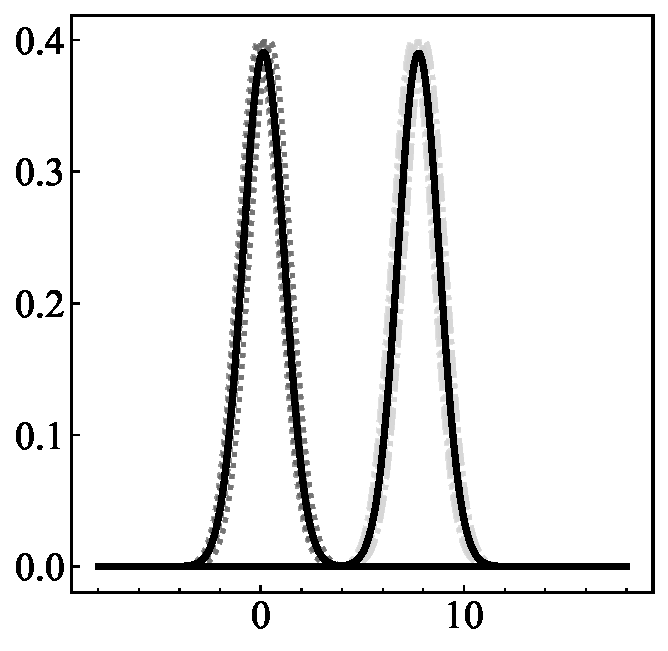
\includegraphics[width=\linewidth]{FCF_IR1_STD0.3.pdf}
					\caption{Tỷ lệ IR $1:1$, tỷ lệ nhiễu $0.5:1$}
	\end{subfigure}
		\begin{subfigure}{.32\textwidth}
		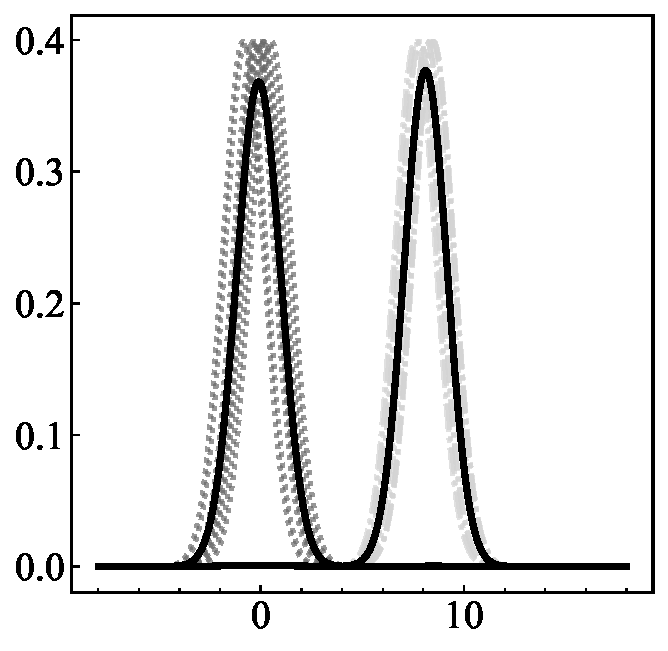
\includegraphics[width=\linewidth]{FCF_IR1_STD0.5.pdf}
					\caption{Tỷ lệ IR $1:1$, tỷ lệ nhiễu $1:1$}
	\end{subfigure}
		\begin{subfigure}{.32\textwidth}
		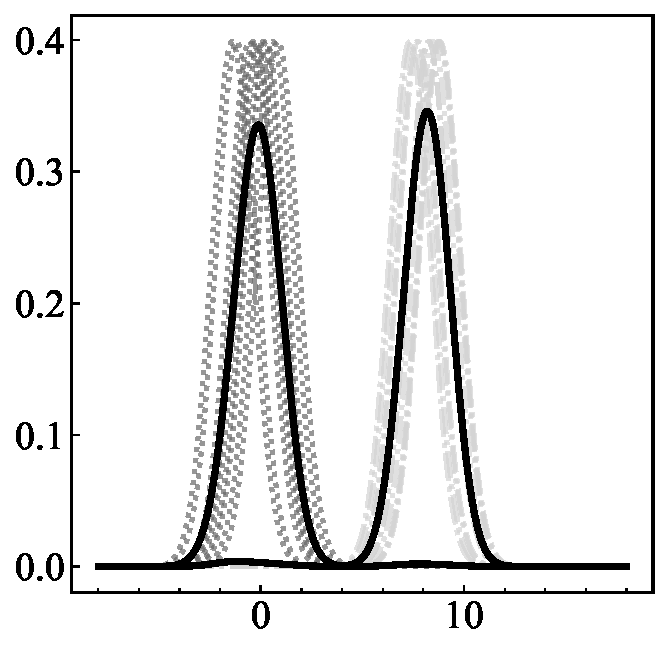
\includegraphics[width=\linewidth]{FCF_IR1_STD0.8.pdf}
			\caption{Tỷ lệ IR $1:1$, tỷ lệ nhiễu $1.5:1$}
	\end{subfigure}\hfill\\
		\begin{subfigure}{.32\textwidth}
		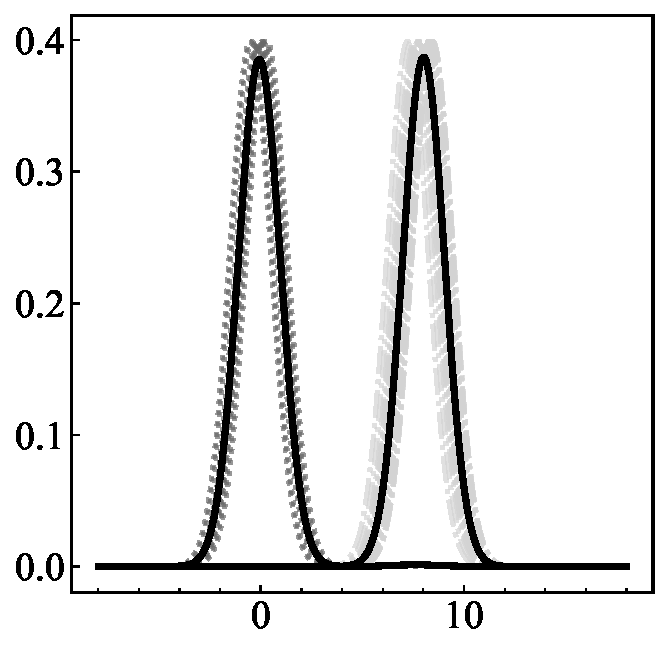
\includegraphics[width=\linewidth]{FCF_IR5_STD0.3.pdf}
					\caption{Tỷ lệ IR $5:1$, tỷ lệ nhiễu $0.5:1$}
	\end{subfigure}
	\begin{subfigure}{.32\textwidth}
		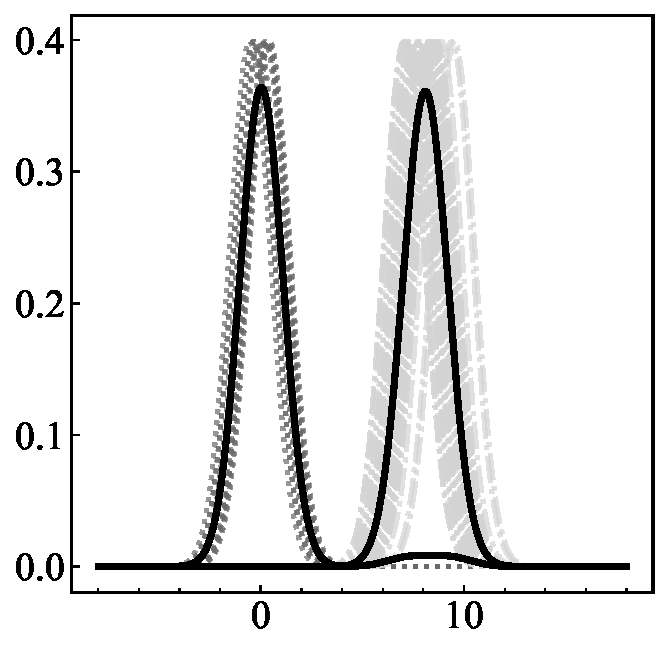
\includegraphics[width=\linewidth]{FCF_IR5_STD0.5.pdf}
							\caption{Tỷ lệ IR $5:1$, tỷ lệ nhiễu $1:1$}
	\end{subfigure}
	\begin{subfigure}{.32\textwidth}
		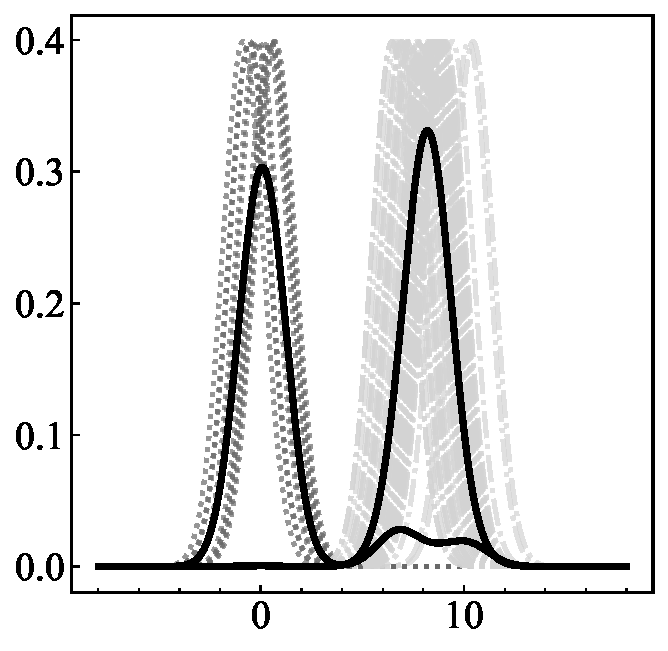
\includegraphics[width=\linewidth]{FCF_IR5_STD0.8.pdf}
					\caption{Tỷ lệ IR $5:1$, tỷ lệ nhiễu $1.5:1$}
	\end{subfigure}\hfill\\
		\begin{subfigure}{.32\textwidth}
		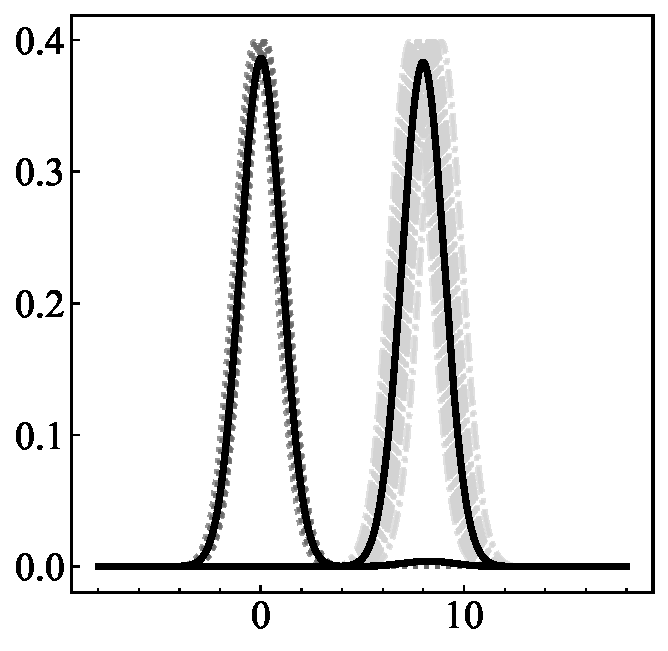
\includegraphics[width=\linewidth]{FCF_IR10_STD0.3.pdf}
							\caption{Tỷ lệ IR $10:1$, tỷ lệ nhiễu $0.5:1$}
	\end{subfigure}
	\begin{subfigure}{.32\textwidth}
		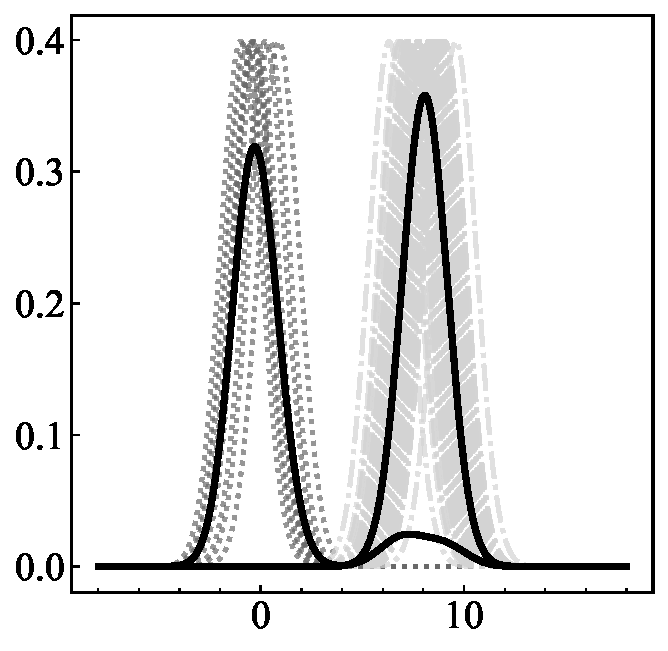
\includegraphics[width=\linewidth]{FCF_IR10_STD0.5.pdf}
							\caption{Tỷ lệ IR $10:1$, tỷ lệ nhiễu $1:1$}
	\end{subfigure}
	\begin{subfigure}{.32\textwidth}
		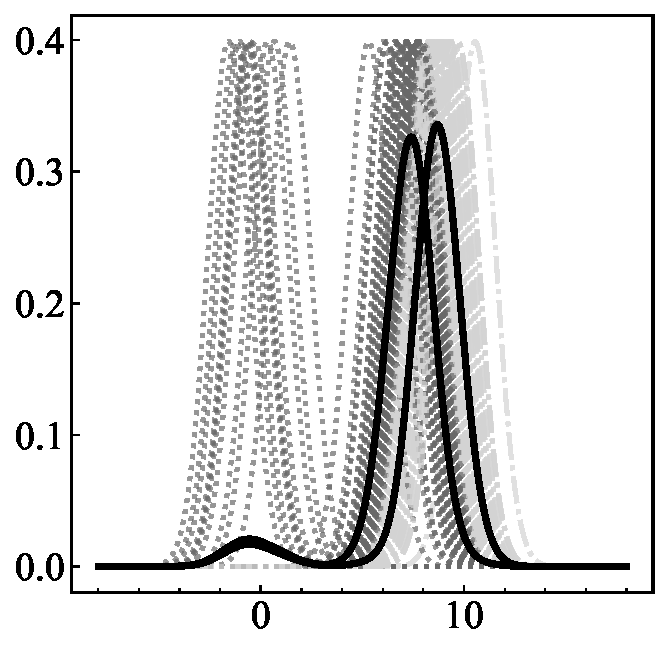
\includegraphics[width=\linewidth]{FCF_IR10_STD0.8.pdf}
					\caption{Tỷ lệ IR $10:1$, tỷ lệ nhiễu $1.5:1$}
	\end{subfigure}\hfill\\
	\begin{subfigure}{.32\textwidth}
	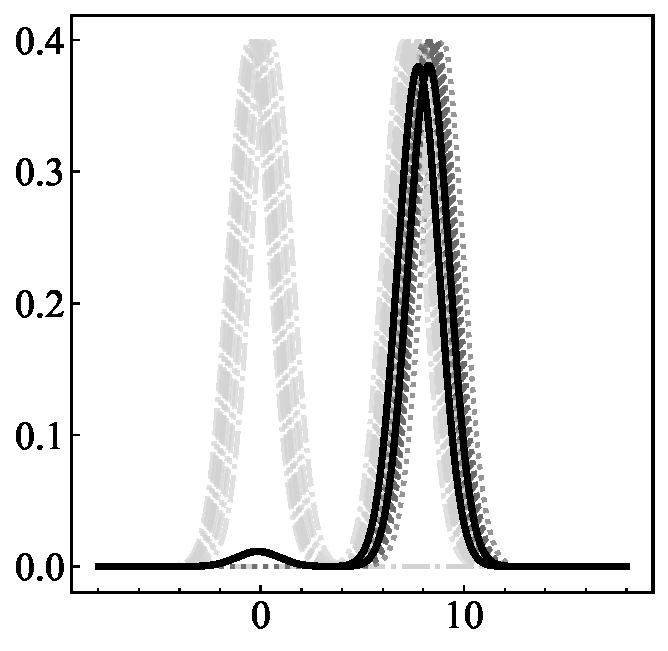
\includegraphics[width=\linewidth]{FCF_IR20_STD0.3.pdf}
						\caption{Tỷ lệ IR $20:1$, tỷ lệ nhiễu $0.5:1$}
	\end{subfigure}
	\begin{subfigure}{.32\textwidth}
	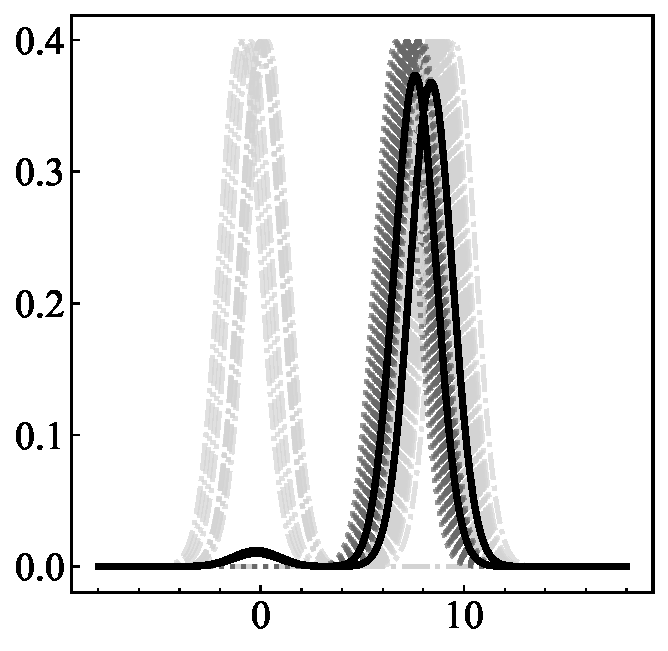
\includegraphics[width=\linewidth]{FCF_IR20_STD0.5.pdf}
						\caption{Tỷ lệ IR $20:1$, tỷ lệ nhiễu $1:1$}
	\end{subfigure}
	\begin{subfigure}{.32\textwidth}
	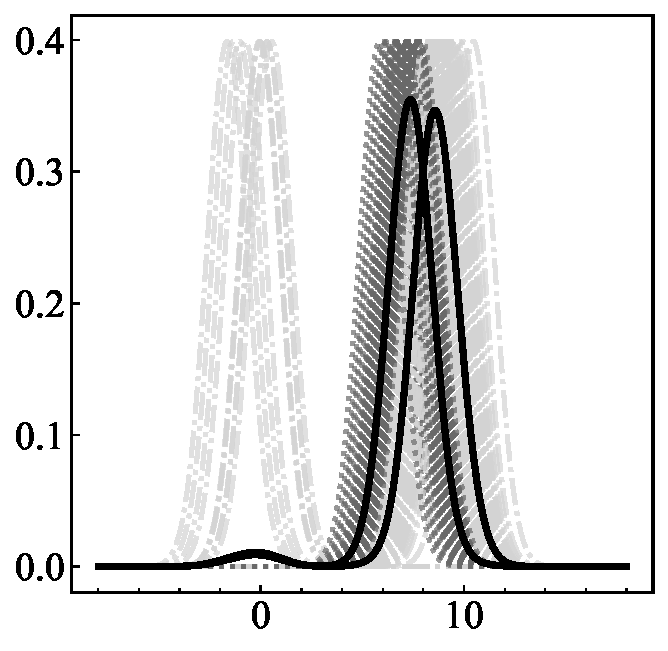
\includegraphics[width=\linewidth]{FCF_IR20_STD0.8.pdf}
						\caption{Tỷ lệ IR $20:1$, tỷ lệ nhiễu $1.5:1$}
	\end{subfigure}
	\caption{Ảnh hưởng của dữ liệu hàm mật độ Gauss mất cân bằng lên FCF ($m=2\,;c=3\,;\bm D=\mathcal{L}_2$)}\label{fig:IR_STD}
\end{figure}

Giả sử hai chùm có số lượng phần tử $\#c_1$ lớn và $\#c_2$ có số lượng nhỏ sao cho $\#c_1=IR\cdot\#c_2$ với $IR\in\mathbb{N}_{>0}$. Khi $IR$ tăng lên, hàm tỷ số giữa $\#c_1$ và tổng số phần tử trong dữ liệu được biểu diễn bởi $k(x) = 1-1/(x+1)$. Ta thấy, hàm $k(x)$ là một đường cong tăng đơn điệu và đạo hàm của nó giảm khi $IR$ tăng. Điều này nghĩa là chỉ số hoá theo kích thước chùm thông qua trọng số lớp trở nên bão hoà. Do đó, cần thiết xây dựng bổ sung việc trung hòa các phần tử trong lớp lớn trong hàm mục tiêu.

\begin{figure}[H] 
	\centering
	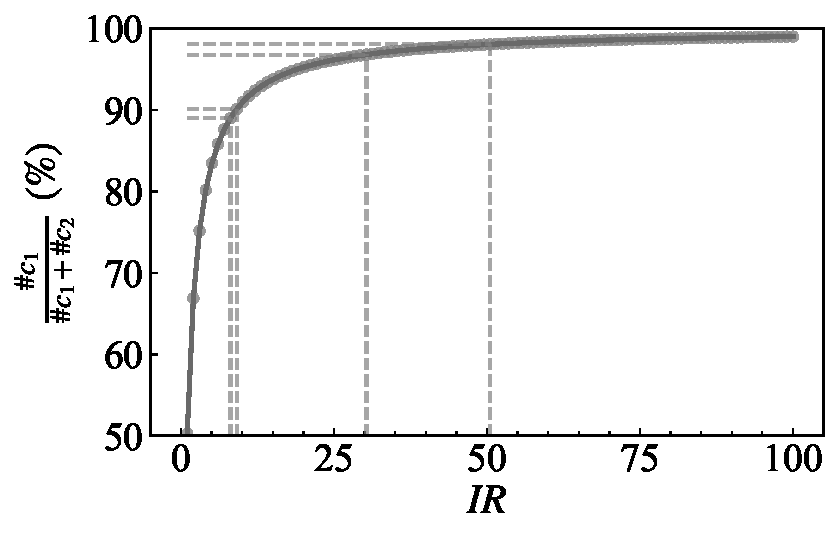
\includegraphics[width=0.6\linewidth]{ratio_C1_k.pdf}
\end{figure}



\subsection{Thuật toán}



Cho tập các hàm mật độ xác suất $\mathcal{F}=\{f_1\,;f_2\,;\ldots\,;f_n\}$, trong đó mỗi $f_j$ là một hàm mật độ xác suất ($j=1\,;\ldots\,;n$). Cho trước $c$ là số chùm ($i=1\,;\ldots\,;c$). Gọi $\bm U=[\mu_{ij}]\in\mathbb{R}^{n\times c}$ là ma trận phân vùng, và $\Theta=\{\theta_1,\dots,\theta_c\}$ là các trọng tâm chùm. Giả sử tham số mờ $m>1$; và $\delta'>0$ là siêu tham số điều khiển các hàm ở biên của chùm.



Hàm mục tiêu của IFCF là tổng của hai phần bao gồm trọng số $1/\omega_i$ giảm ``hiệu ứng đồng nhất''.
\begin{align}
	\tag{IFCF}\label{eq:IFCF}
\text{Minimise}\,&:\, J(\bm U\,;\Theta\,|\, \mathcal{F}\,;c\,;m\,;\delta') = 
	\underbrace{\sum_{j=1}^n \sum_{i=1}^c \frac{1}{\omega_i}\, \mu_{ij}^m \,D^2(f_j\,;\theta_i)}_{IFCF},\\
		\text{s.t}\,&:\,\sum_{i=1}^{c} \mu_{ij} = 1,\quad \forall j \in {1, \dots, n}, \tag{C1}\label{c1_pro} 
\end{align}
trong đó $\omega_i=\frac{1}{n}\sum_{j=1}^n \mu^{(t-1)}_{ij}$ là tỷ lệ kích thước mờ của chùm thứ $i$, với $1\,;\ldots\,c$, thỏa mãn $\sum_{i=1}^c\omega_i=1$ với $\mu^{(t-1)}_{ij}$ là ma trận phân vùng tại vòng lặp thứ $(t-1)$.
Khi $\omega_i= \bm 1$ thì thuật toán trở thành FCF. 

\chy{
	Khi mất cân bằng tăng, đóng góp của chùm lớn hơn vào hàm mục tiêu sẽ lấn át chùm nhỏ hơn. Do đó, thành phần $IFCF$ chia cho $\tfrac{1}{\omega_i}$, với $\omega_i\in(0\,;1)$ sẽ giảm một tỷ lệ kích thước chùm cho cả hai bên. Khi đó, chùm lớn phải chịu tổn thất lớn hơn để giảm đóng góp hàm mục tiêu mà không làm sai lệch trọng tâm và tính ổn định.
	}



%
%Hàm mục tiêu của IFCF là tổng của hai phần bao gồm trọng số $1/\omega_i$ giảm ``hiệu ứng đồng nhất'' và hiệu chỉnh biên \index{hiệu chỉnh biên (edge modification)} giảm ``hiệu ứng xi-phông''.
%\begin{align}
%	\tag{IFCF}\label{eq:EMIFCF}
%\text{Minimise}\,&:\, J(\bm U\,;\Theta\,|\, \mathcal{F}\,;c\,;m\,;\delta') = 
%	\underbrace{\sum_{j=1}^n \sum_{i=1}^c \frac{1}{\omega_i}\, \mu_{ij}^m \,D^2(f_j\,;\theta_i)}_{IFCF}
%	\;+\;
%\underbrace{	\sum_{j=1}^n \delta_j \sum_{i=1}^c \mu_{ij}\bigl(1-\mu_{ij}^{\,m-1}\bigr)\, D^*_{ij}}_{EM},\\
%		\text{s.t}\,&:\,\sum_{i=1}^{c} \mu_{ij} = 1,\quad \forall j \in {1, \dots, n}, \tag{C1}\label{c1_pro} 
%\end{align}
%trong đó $\omega_i=\frac{1}{n}\sum_{j=1}^n \mu^{(t-1)}_{ij}$ là tỷ lệ kích thước mờ của chùm thứ $i$, với $1\,;\ldots\,c$, thỏa mãn $\sum_{i=1}^c\omega_i=1$ với $\mu^{(t-1)}_{ij}$ là ma trận phân vùng tại vòng lặp thứ $(t-1)$, và $D^*_{ij}$ là chuẩn hóa  $[0\,;1]$ của ma trận khoảng cách ở vòng lặp trước được tính bởi
%\begin{align}
%	D^{*^{(t-1)}}(\theta_i\,,f_j)\;=\;\frac{D^2\left (\theta_i^{(t-1)}\,;f_j\right )}{\sum_{s=1}^c D^2\left (\theta_s^{(t-1)}\,;f_j\right)},	\label{eq:Dstar}
%\end{align}
%và $\delta_j$ là hệ số điều khiển. 
%Khi $\omega_i= \bm 1$ và $\delta'=0$ thì thuật toán trở thành FCF. 
%
%\chy{
%Khi mất cân bằng tăng, đóng góp của chùm lớn hơn vào hàm mục tiêu sẽ lấn át chùm nhỏ hơn. Do đó, thành phần $IFCF$ chia cho $\tfrac{1}{\omega_i}$, với $\omega_i\in(0\,;1)$ sẽ giảm một tỷ lệ kích thước chùm cho cả hai bên. Khi đó, chùm lớn phải chịu tổn thất lớn hơn  để giảm đóng góp hàm mục tiêu mà không làm sai lệch trọng tâm và tính ổn định.
%
%Tuy nhiên, việc chuẩn hoá kích thước chùm không phân biệt được mức độ khó của từng hàm mật độ tại các biên của chùm, nơi khởi phát hiệu ứng xi phong. Do đó, số hạng EM tim kiếm các hàm biên thông qua hệ số $
%\mu_{ij}\bigl(1-\mu_{ij}^{\,m-1}\bigr)
%$. Nó tiến gần $0$ với biên và lớn hơn khi không phải. Đồng thời, nhân tử $D^{*}_{ij}$ cung cấp hướng phạt làm triệt tiêu xu hướng hút của hiệu ứng xi phông.
%
%}
%
%
%
\subsection{Sự hội tụ của thuật toán}
%
Trong phần này, một dãy ${\left (\bm\mu^{(t)}\,; \Theta^{(t)} \right )}$ khởi tạo được thành lập. Mục tiêu là chứng minh dãy này có hội tụ hay không \cite{bezdek1980convergence,yu2024suppressed}.  Cho
 $
F\,:\,\mathbb{R}^{cd} \to \bm{U}_f\,; F(\Theta) = \bm{\mu}\,; \text{và }
G\,:\,\bm{U}_f \to \mathbb{R}^{cd} \,; G(\bm{\mu})=\Theta$, trong đó, $\Theta = (\theta_1\,;\theta_2\,; \ldots\,;\theta_c)$ và các hàm mật độ trọng tâm $\theta_i$ tính bởi công thức \eqref{trongtamFCF}. Ta định nghĩa toán tử $T_{IFCF}\,:\,\mathbb{R}^{cd} \times \bm{U}_f\to \mathbb{R}^{cd} \times \bm{U}_f\,; T_{ IFCF} = T_2\circ T_1,$ trong đó ánh xạ  $T_1\,:\,\mathbb{R}^{cd} \times \bm{U}_f \to \mathbb{R}^{cd} \,; T_1(\bm{\mu} \,;\Theta)=G(\bm \mu)$, và $T_2\,:\, \mathbb{R}^{cd} \to \mathbb{R}^{cd}\times\bm{U}_f \,; T_2(\Theta)= (F(\Theta), \Theta)$. Khi này, ta có $T_{ IFCF} = (T_2\circ T_1)\left(F\circ G(\mu)\,;G(\mu)\right)$. Tức là
 \begin{align}\label{TO}
	T_{IFCF}\,:\,\mathbb{R}^{cd} \times \bm{U}_f\to \mathbb{R}^{cd} \times \bm{U}_f\,; T_{IFCF} = T_2\circ T_1,
\end{align}
%
%
%
%%==================== LEMMA 1: Cập nhật ma trận phân vùng U ====================

\bode{[Cập nhật ma trận phân vùng $\bm U$]\label{lem1}
	Với $\Theta$ cố định, bài toán tối ưu hoá $J_{IFCF}$ theo $\bm U=[\mu_{ij}]$ có nghiệm cực tiểu duy nhất $\bm U^*=F(\Theta)$ dưới các ràng buộc phân hoạch mờ \eqref{c1_pro}. Cụ thể,
	\begin{align}
		\mu_{ij} \;=\;
		\frac{
			\left[\frac{\omega_i}{\,D^2(\theta_i,f_j)}\right]^{\frac{1}{m-1}}
		}{
			\sum_{s=1}^c
			\left[\frac{\omega_s}{\,D^2(\theta_s,f_j)}\right]^{\frac{1}{m-1}}
		}\,;
		1\le i\le c,\;1\le j\le n,
		\label{eq:ifcf_u_final}
	\end{align}
	trong đó $\omega_i=\tfrac{1}{n}\sum_{j=1}^n \mu^{(t-1)}_{ij}$ là trọng số kích thước chùm với $\omega_i>0$, $i=1,\dots,c$ và $\sum_i \omega_i=1$. Ngoài ra, nếu tồn tại $i_0$ sao cho $D^2(\theta_{i_0},f_j)=0$ thì nghiệm tối ưu cho cột $j$ là $\mu_{i_0 j}=1$ và $\mu_{s j}=0$ với mọi $s\neq i_0$; nếu có nhiều chỉ số đạt $0$ thì mọi phân phối trên tập đó đều tối ưu.}


\chm{Do ràng buộc phân hoạch mờ là độc lập theo từng mẫu $j$, và mục tiêu \eqref{eq:IFCF} là tổng theo $j$, bài toán tối ưu hoá theo $\bm U$ tách thành $n$ bài toán độc lập. 
	Cố định một $j\in\{1,\dots,n\}$, đặt hằng số
	$
	\delta_{ij}\coloneq D^2(\theta_i,f_j)/\omega_i.
	$	
	Khi này, mục tiêu của bài toán con theo cột $j$ là
	\begin{align}
		\min_{\mu_{\cdot j}\in\mathbb R_{>0}^c}\ \ \phi_j(\mu_{\cdot j})\,:\,\sum_{i=1}^c \delta_{ij}\,\mu_{ij}^m
		\quad\text{s.t.}\quad
		\sum_{i=1}^c \mu_{ij}=1,\ \mu_{ij}\ge 0.
		\label{eq:subprob}
	\end{align}
	
	Với $m>1$, ta nhận được hàm $t\mapsto t^m$ lồi nghiêm ngặt trên $\mathbb R_{>0}$. Khi đó, hàm mục tiêu $\phi_j$ là tổng các hàm lồi nghiêm ngặt theo từng biến. Miền khả thi là một đơn hình đóng và bị chặn, do đó nghiệm tối ưu tồn tại duy nhất. Hơn nữa, ma trận Hessian là xác định dương, với các phần tử trong ma trận
	$$
	\frac{\partial^2 \phi_j}{\partial \mu_{ij}^2}=m(m-1)(\delta_{ij})\mu_{ij}^{m-2}>0\,,
	\frac{\partial^2 \phi_j}{\partial \mu_{ij}\partial \mu_{sj}}=0\ (s\neq i),
	$$
	
	Lập Lagrangian với nhân tử $\lambda_j\in\mathbb R$ cho ràng buộc tổng bằng $1$ và $\alpha_{ij}\ge 0$ cho các ràng buộc không âm, ta có
	\begin{align}
		\mathcal L(\mu_{\cdot j},\lambda_j,\alpha_{\cdot j})
		&=
		J_{IFCF} 
		-\lambda_j\Bigl(\sum_{i=1}^c \mu_{ij}-1\Bigr)
		-\sum_{i=1}^c \alpha_{ij}\,\mu_{ij}.
		\label{eq:L_ifcf}
	\end{align}
	Điều kiện dừng bậc nhất là đạo hàm riêng của \eqref{eq:L_ifcf} theo $\mu_{ij}$ bằng $0$.
	\begin{align}\label{eq:stat-KKT}
		\frac{\partial}{\partial \mu_{ij}}\mathcal L
		=
		m\,\delta_{ij}\,\mu_{ij}^{m-1}
		-\lambda_j-\alpha_{ij}
		=0,
			\end{align}
	cùng với các điều kiện $
	\sum_{i=1}^c \mu_{ij}=1$, $
	\mu_{ij}\ge 0,\ \alpha_{ij}\ge 0$,  và $ 
	\alpha_{ij}\mu_{ij}=0,\ \forall i.$
	Giả sử $\delta_{ij}>0$ với mọi $i$, nếu $\mu_{ij}>0$ thì $\alpha_{ij}=0$. Khi đó \eqref{eq:stat-KKT} cho kết quả
	\begin{align}
		\mu_{ij}=\Bigl(\frac{\lambda_j}{m}\Bigr)^{\frac{1}{m-1}}(\delta_{ij})^{-\frac{1}{m-1}}.
		\label{eq:mu-lambda-c}
	\end{align}
	
	Áp dụng ràng buộc chuẩn hoá $\sum_{i=1}^c \mu_{ij}=1$ vào \eqref{eq:mu-lambda-c}, ta có
	\begin{align*}
		1
		=\sum_{i=1}^c \Bigl(\frac{\lambda_j}{m}\Bigr)^{\frac{1}{m-1}}(\delta_{ij})^{-\frac{1}{m-1}}
		=\Bigl(\frac{\lambda_j}{m}\Bigr)^{\frac{1}{m-1}}
		\sum_{i=1}^c (\delta_{ij})^{-\frac{1}{m-1}},
	\end{align*}
	suy ra
	$$
	\Bigl(\frac{\lambda_j}{m}\Bigr)^{\frac{1}{m-1}}
	=\frac{1}{\sum_{s=1}^c (\delta_{sj})^{-\frac{1}{m-1}}}.
	$$
	Thế ngược lại vào \eqref{eq:mu-lambda-c}, ta thu được \eqref{eq:ifcf_u_final}.

	Ngược lại, tồn tại $i_0$ sao cho $D^2(\theta_{i_0},f_j)=0$ thì $\delta_{i_0 j}=0$. Tuy nhiên, với mọi $s\neq i_0$, $\delta_{sj}>0$, nên để tối thiểu hoá tổng $\sum_s c_{sj}\mu_{sj}^m$ dưới ràng buộc tổng bằng 1, nghiệm tối ưu là $\mu_{i_0 j}=1$ và $\mu_{s j}=0$ với $s\neq i_0$. Từ đây, ta được điều phải chứng minh.	
	}




%\bode{[Cập nhật ma trận phân vùng $\bm U$]\label{lem1}
%	Với $\Theta$ cố định, bài toán tối ưu hoá $J_{IFCF}$ theo $\bm U=[\mu_{ij}]$ có nghiệm cực tiểu duy nhất $\bm U^*=F(\Theta)$ dưới các ràng buộc phân hoạch mờ \eqref{c1_pro}. Cụ thể,
%	\begin{align}
%		\mu_{ij} \;=\;
%		\frac{
%			\left[\dfrac{(1-\delta' D^{*}_{ij})\,\omega_i}{\,D^2(\theta_i,f_j)\;-\;f_j\,\delta_j\,D^{*}_{ij}\,}\right]^{\frac{1}{m-1}}
%		}{
%			\displaystyle\sum_{s=1}^c
%			\left[\dfrac{(1-\delta' D^{*}_{sj})\,\omega_i}{\,D^2(\theta_s,f_j)\;-\;\omega_i\,\delta_j\,D^{*}_{sj}\,}\right]^{\frac{1}{m-1}}
%		}\,;
%		  1\le i\le c,\;1\le j\le n,
%		\label{eq:emifcf_u_final}
%	\end{align}
%	trong đó $\delta_j=\delta'\lambda_j$, và $D^{*}_{ij}$ được tính theo các trọng tâm ở vòng lặp trước, và $\omega_i>0\,;i=1\,;\ldots\,;c$ là trọng số kích thước chùm.}
%
%\chm{
%	Xét $J_{IFCF}$ ở bước cập nhật $U$ (giữ $\Theta$ cố định). Phần phụ thuộc vào $U$ có dạng
%	\[
%	J_U(\bm U) \;=\; 
%	\sum_{j=1}^n \sum_{i=1}^c 
%	\frac{1}{\omega_i}\,\mu_{ij}^{\,m}\,D^2(\theta_i,f_j)
%	\;+\;\sum_{j=1}^n \delta_j\,\mu_{ij}\bigl(1-\mu_{ij}^{\,m-1}\bigr)\,D^{*}_{ij},
%	\]
%	với ràng buộc mờ $
%	\sum_{i=1}^c \mu_{ij}=1$ và $\mu_{ij}\ge\,;\forall\,j=1,\dots,n.$
%	
%	Lập hàm Lagrange $\mathcal{L}$ với các nhân tử $\{\lambda_j\}_{j=1}^n$ cho ràng buộc tổng bằng 1, và $\{\alpha_{ij}\ge0\}$ cho ràng buộc không âm. Ta có
%	\begin{align}\label{eq:L_em}
%	\mathcal{L}(\bm U,\lambda,\alpha)
%	=
%J_{IFCF}(\bm U\,;\Theta) 
%	-\sum_{j=1}^n \lambda_j\Bigl(\sum_{i=1}^c \mu_{ij}-1\Bigr)
%	-\sum_{j=1}^n\sum_{i=1}^c \alpha_{ij}\,\mu_{ij}.
%	\end{align}
%	
%	Lấy đạo hàm riêng của \eqref{eq:L_em} theo $\mu_{ij}$ và cho đạo hàm bằng $0$, ta có
%	\begin{align}
%		\frac{\partial}{\partial \mu_{ij}}\mathcal{L}(\bm U\,;\lambda\,;\alpha)
%		&=
%		\frac{1}{\omega_i}\,m\mu_{ij}^{\,m-1} D^2(\theta_i,f_j)
%		+\delta_j\,\Bigl(1-m\mu_{ij}^{\,m-1}\Bigr)\,D^{*}_{ij}
%		-\lambda_j-\alpha_{ij}
%		\;=\;0.
%		\label{eq:stat_raw}
%	\end{align}
%Ta suy ra được
%	\[
%	m\mu_{ij}^{\,m-1}\!\left(\frac{1}{\omega_i} D^2(\theta_i,f_j)-\delta_j D^{*}_{ij}\right)
%	=\lambda_j+\alpha_{ij}-\delta_j D^{*}_{ij}.
%	\]
%	Với nghiệm trong miền khi $D^2>0$, $1-\delta' D^{*}_{ij}>0$, ta có $\mu_{ij}>0$ nên theo KKT–3 ta suy ra $\alpha_{ij}=0$. Khi đó,
%	\begin{align}
%		\mu_{ij}^{\,m-1}
%		=
%		\frac{\lambda_j-\delta_j D^{*}_{ij}}
%		{m\left(\frac{1}{\omega_i} D^2(\theta_i,f_j)-\delta_j D^{*}_{ij}\right)}
%		\Rightarrow
%		\mu_{ij}
%		=
%		\left[
%		\frac{(\lambda_j-\delta_j D^{*}_{ij})\,\omega_i}
%		{m\bigl(D^2(\theta_i,f_j)-\omega_i\,\delta_j D^{*}_{ij}\bigr)}
%		\right]^{\frac{1}{m-1}}.
%		\label{eq:mu_lj_form}
%	\end{align}
%	
%	Ngoài ra, $
%	\sum_{i=1}^c \mu_{ij}=1,\;\mu_{ij}\ge0.$ và $
%	\alpha_{ij}\ge 0,\;
%	\alpha_{ij}\,\mu_{ij}=0.$
%	Thế \eqref{eq:mu_lj_form} vào $\sum_{i=1}^c\mu_{ij}=1$ ta được
%	\begin{align}\label{eq:lambda_1}
%	1
%	=
%	\sum_{i=1}^c
%	\left[
%	\frac{(\lambda_j-\delta_j D^{*}_{ij})\,\omega_i}
%	{m\bigl(D^2(\theta_i,f_j)-\omega_i\,\delta_j D^{*}_{ij}\bigr)}
%	\right]^{\frac{1}{m-1}}
%	\!\!.
%	\end{align}
%	Giải phương trình \eqref{eq:lambda_1} theo $\lambda_j$ và đặt $\delta_j=\delta'\lambda_j$, ta được
%	\[
%	\mu_{ij}
%	=
%	\lambda_j^{\frac{1}{m-1}}
%	\left[
%	\frac{(1-\delta' D^{*}_{ij})\,\omega_i}
%	{m\bigl(D^2(\theta_i,f_j)-\omega_i\,\delta_j D^{*}_{ij}\bigr)}
%	\right]^{\frac{1}{m-1}}.
%	\]
%Từ đây khi hệ số $m>1$, triệt tiêu giữa tử và mẫu, dẫn đến \eqref{eq:emifcf_u_final} ta thu được công thức như Bổ đề \ref{lem1}.
%	
%	Với $\Theta$ cố định, $J(\bm U)$ là lồi nghiêm ngặt theo từng cột $\mu_{\cdot j}$ trên miền đơn hình không âm khi các mẫu số dương, ta có $
%	D^2(\theta_i,f_j)-\omega_j\,\delta_j\,D^{*}_{ij}>0
%	\text{ và }
%	1-\delta' D^{*}_{ij}>0.$ Do đó nghiệm KKT là duy nhất và là cực tiểu toàn cục cho bài toán theo $\bm U$. 
%}
%
%==================== LEMMA 2: Cập nhật trọng tâm Theta ====================
\bode{[Cập nhật trọng tâm $\Theta$ với $\mathcal{L}_2^2$]\label{lem2}
	Với $\bm U$ cố định, bài toán tối thiểu hoá $J_{IFCF}$ theo $\Theta=\{\theta_i\}_{i=1}^c$ là phân tích được theo từng $\theta_i$ và lồi nghiêm ngặt. Tồn tại duy nhất nghiệm cực tiểu $\Theta^*=G(\bm U)$ khi khoảng cách $D^2=\mathcal{L}_2^2$, 
	\begin{align}
		\theta_i
		\;=\;
		\frac{\sum_{j=1}^n (\mu_{ij})^{m}\,f_j}
		{\sum_{j=1}^n (\mu_{ij})^{m}}\,;
		 1\le i\le c,
		\label{eq:theta_update}
	\end{align}
}

\chm{
	Giữ $U$ cố định, lấy đạo hàm $\psi_i=\sum_{i=1}^c \psi_i(\theta_i),$ với các $\psi_i(\theta_i)=\sum_{j=1}^n \frac{1}{\omega_i}\,(\mu_{ij})^{m}\,D^2(\theta_i\,,f_j).$ theo $\theta_i$ đối với hàm mục tiêu \eqref{eq:IFCF} ta có
	\begin{align}\label{eq:théta}
	\nabla_{\theta_i}\psi_i(\theta_i)
	=
	\frac{1}{\omega_i}\sum_{j=1}^n
	(\mu_{ij})^{m}(\mu_{ij})^{m}\nabla\theta_i\mathcal{L}_2^2(\theta_i\,,f_j)
	\end{align}
	Cho $\nabla_{\theta_i}\psi_i(\theta_i)=\bm 0$, ta được công thức cập nhật  \eqref{eq:theta_update} đối với riêng trường hợp $\mathcal{L}_2^2(\theta_i\,,f_j)$.
	Hơn nữa, với khoảng cách $\mathcal{L}_2$, ma trận Hess theo $\theta_i$ là
	$
	\nabla^2_{\theta_i}\psi_i(\theta_i)
	=
	\frac{2}{\omega_i}\left(\sum_{j=1}^n (\mu_{ij})^{m}\right)\,\bm I_d,
	$ xác định dương vì $\sum_j (\mu_{ij})^{m}>0$ và $\omega_i>0$. Do đó $\psi_i$ lồi nghiêm ngặt và nghiệm bậc nhất \eqref{eq:théta} là duy nhất, suy ra nghiệm toàn cục duy nhất $\Theta^*=G(\bm U)$. Tuy nhiên, $	\nabla^2_{\theta_i}\psi_i(\theta_i)$ chỉ lồi nghiêm ngặt trong một số khoảng cách như $\mathcal{L}_2\,, D^2_H\,, D_{KL}$ hoặc $W_2$, trong khi với các khoảng cách khác bao gồm $\mathcal{L}_2, D_B$ hoặc $D_M$ có thể không duy nhất nghiệm toàn cục.
}

\bode{[Cập nhật trọng tâm $\Theta$ với $D_H^2$]\label{lem:Hellinger}
	Với $\bm U$ cố định, bài toán tối thiểu hoá $J_{IFCF}$ theo $\Theta=\{\theta_i\}_{i=1}^c$ có thể tách được theo từng $\theta_i$ và là lồi nghiêm ngặt trong biến $\sqrt{\theta_i}$. 
	Tồn tại duy nhất nghiệm cực tiểu $\Theta^*=G(\bm U)$ khi khoảng cách $D^2=D_H^2$, trong đó 
	\begin{align}
		\theta_i(x)
		\;=\;
		\frac{\Big(\sum_{j=1}^n (\mu_{ij})^{m}\,\sqrt{f_j(x)}\Big)^2}
		{ \int_{\Omega} \Big(\sum_{j=1}^n (\mu_{ij})^{m}\,\sqrt{f_j(y)}\Big)^2\,\mathrm{\,d}y}, 
		\qquad 1\le i\le c.
		\label{eq:theta_update_H}
	\end{align}
}

\chm{
	Giữ $U$ cố định, xét $\psi_i(\theta_i)=\sum_{j=1}^n \frac{1}{\omega_i}\,(\mu_{ij})^{m}\,D_H^2(\theta_i,f_j)$. 
	Ta có khoảng các bình phương Hellinger là $
	D_H^2(\theta_i,f_j) \;=\; 1 - \int \sqrt{\theta_i(x)\,f_j(x)}\mathrm{\,d}x.$	
	Do đó
	\[
	\psi_i(\theta_i)
	= \frac{1}{\omega_i}\sum_{j=1}^n (\mu_{ij})^m \left(1-\int_{\Omega} \sqrt{\theta_i(x)\,f_j(x)}\,\mathrm{\,d}x\right).
	\]

	Vì $\theta(x)\le 0$, đặt $g_i(x)=\theta_i^{1/2}(x)$. Khi đó $\psi_i$ trở thành một hàm lồi theo $g_i$. Vì vậy,
	\[
	\frac{\delta \psi_i}{\delta g_i(x)} 
	= -\frac{1}{\omega_i}\sum_{j=1}^n (\mu_{ij})^m \sqrt{f_j(x)} \;+\; \frac{1}{\omega_i}\Big(\sum_{j=1}^n (\mu_{ij})^m\Big) g_i(x).
	\]
	
	Cho $\frac{\delta \psi_i}{\delta g_i(x)}=0$ và $\theta_i(x)=g_i^2(x)$, ta dẫn đến công thức \eqref{eq:theta_update_H}. Ta cũng có ma trận Hess lúc này là xác định dương, nghiệm \eqref{eq:theta_update_H} là nghiệm toàn cục duy nhất.
}



Ta cũng chứng minh được công thức đóng tại Bổ đề~\ref{lem:Hellinger} cũng là một hàm mật độ xác suất.

\chm{
Từ kết quả công thức~\eqref{eq:theta_update_H}, ta có
\[
\int_{\Omega}\theta_i(x)\,\mathrm{d}x
=\int_{\Omega}\frac{\Big(\sum_{j=1}^n (\mu_{ij})^{m}\,\sqrt{f_j(x)}\Big)^2}
{ \int_{\Omega}\Big(\sum_{j=1}^n (\mu_{ij})^{m}\,\sqrt{f_j(y)}\Big)^2\,\mathrm{d}y}
\,\mathrm{d}x=\frac{ \int_{\Omega}\Big(\sum_{j=1}^n (\mu_{ij})^{m}\,\sqrt{f_j(x)}\Big)^2\,\mathrm{d}x}
{ \int_{\Omega}\Big(\sum_{j=1}^n (\mu_{ij})^{m}\,\sqrt{f_j(y)}\Big)^2\,\mathrm{d}y}=1.
\]

}




Bảng~\ref{tab:KCTT} trình bày các công thức cập nhật trọng tâm $\theta$ của chùm theo những khoảng cách khác nhau. 

\begin{table}[H]
	\centering
	\scriptsize
	\caption{Các công thức trọng tâm tương ứng với các loại khoảng cách}\label{tab:KCTT}
	\begin{tabular*}{\textwidth}{@{\extracolsep\fill}ll@{\extracolsep\fill}}
		\toprule
	\textbf{Công thức khoảng cách} & \textbf{Trọng tâm $\theta$} \\
		\midrule
 $\mathcal{L}^2(f,\theta)=\int (f(x)-\theta(x))^2\mathrm{\,d}x$ 
		& $\displaystyle\theta(x) = \frac{\sum_j u_{ij}^m f_j(x)}{\sum_j u_{ij}^m}$ \\
$D_H^2(f,\theta)=\tfrac{1}{2}\int \big(\sqrt{f(x)}-\sqrt{\theta(x)}\big)^2 \mathrm{\,d}x$ 
		& $\displaystyle\theta(x)= \left(\frac{\sum_j u_{ij}^m \sqrt{f_j(x)}}{\sum_j u_{ij}^m}\right)^2$ \\
 $W_2^2(f,\theta) = \int_0^1 \big(F^{-1}(p)-G^{-1}(p)\big)^2 \mathrm{\,d}p$,
		& $\displaystyle\theta(x)=\frac{\mathrm{\,d}}{\mathrm{\,d}x}Q_\theta^{-1}\,, Q_\theta(p) = \frac{\sum_j u_{ij}^m Q_{f_j}(p)}{\sum_j u_{ij}^m}$ \\
		\bottomrule
	\end{tabular*}
\end{table}

\begin{figure}[H]
	\centering
	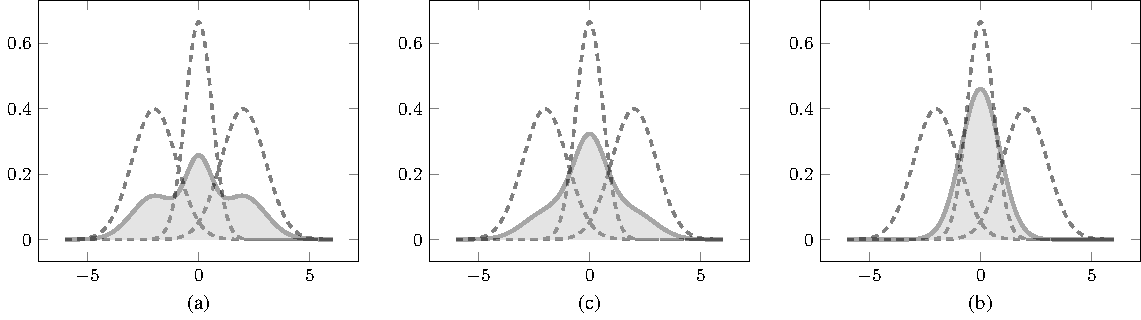
\includegraphics[width=\linewidth]{C2_hamtrongtam}
	\begin{flushleft}
		\it\footnotesize Ghi chú từng loại khoảng cách (a) $\mathcal{L}_2$, (b) Hellinger và (c) Wasserstein-2.
	\end{flushleft}
	\caption[Minh họa các công thức trọng tâm theo khoảng cách]{Minh họa các công thức trọng tâm theo khoảng cách}
\end{figure}


%
%
%
%
%
%
%
%
%
Tuy nhiên, hai bổ đề \ref{lem1} và \ref{lem2} chỉ là điều kiện cần để $(\bm{\mu}^*\,;\Theta^*)$ là một cực tiểu toàn cục của hàm mục tiêu $J_{IFCF}$. Từ đây, câu hỏi tiếp theo là liệu dãy $\{T_{IFCF}^{(t)}(\bm{\mu}^{(0)})\}$ có hội tụ về $\bm{\mu}^*$ hay không. Điều kiện đủ cho định lý Zangwill là tính com-pắc của một tập con $\bm{U}_f \times \mathbb{R}^{cd}$
chứa tất cả các dãy sinh bởi $T_{IFCF}$. 

 
 
Ba định lý này là một phần của chứng minh \eqref{eq:IFCF} bằng định lý Zangwill, chứng minh trực tiếp cho kết quả của Định lý~\ref{theo4}.

\dly{[Ràng buộc com-pắc]\label{theo3}
	Cho $[\mathrm{conv}(\mathcal{F})]^c$ là tích Descartes bậc $c$ của bao lồi $\mathcal{F}$, và $(\bm{\mu}^{(0)}\,;\Theta^{(0)})$ là điểm bắt đầu của phép lặp với $J_{IFCF}$, với $\bm{\mu}^{(0)}\in\bm{U}_f$ và $\Theta^{(0)} = G(\bm{\mu}^{(0)})$. Khi đó
	$T^{(0)}_{IFCF}\left(\bm{\mu}^{(0)}\,;\Theta^{(0)}\right)\in \bm{U}_f\times [\mathrm{conv}(\mathcal{F})]^c,$
	và $\bm{U}_f\times [\mathrm{conv}(\mathcal{F})]^c$ là tập com-pắc trong $\bm{U}_f \times \mathbb{R}^{cd}$. % (sửa từ cn → cd)
}

\chm{
	Giả sử $\bm{\mu}^{(0)}\in\bm{U}_f$, khi đó $\Theta^{(0)} = G(\bm{\mu}^{(0)})$ được tính theo \eqref{eq:theta_update}. Khi đó $\theta^{(0)}_i = \frac{\sum_{j=1}^n\left(\mu^{(0)}_{ij}\right)^mf_j}{\sum_{j=1}^n\left(\mu^{(0)}_{ij}\right)^m}.$
	Đặt $\rho_{ij} = \frac{\left(\mu^{(0)}_{ij}\right)^m}{\sum_{l=1}^n\left(\mu^{(0)}_{il}\right)^m},\; 1\le j\le n$. Theo các ràng buộc \eqref{c1_pro}, ta có $0<\rho_{ij}<1$, $\forall i,j$. Vậy $\forall i$, ta viết lại $\theta^{(0)}_i = \sum_{j=1}^n\rho_{ij}f_j$, với $\sum_{j=1}^n\rho_{ij}=1.$ 
	
	Tóm lại $\forall i,\; \theta^{(0)}_i\in \mathrm{conv}(\mathcal{F})$, và do đó $\Theta^{(0)}\in [\mathrm{conv}(\mathcal{F})]^c$. Tiếp tục đệ quy  $\bm{\mu}^{(1)}=F(\bm{\mu}^{(0)})\in \bm{U}_f$, và $\Theta^{(1)}=G(\bm{\mu}^{(1)})\in [\mathrm{conv}(\mathcal{F})]^c$ theo lập luận tương tự. Do đó, mọi dãy lặp của $J_{IFCF}$ đều thuộc về $\bm{U}_f\times [\mathrm{conv}(\mathcal{F})]^c$ với mọi $t\ge1$. Mặc dù có thể khởi tạo $\Theta^{(0)}\in\mathbb{R}^{cd}\setminus[\mathrm{conv}(\mathcal{F})]^c$, nhưng khi đó $\bm{\mu}^{(0)} = F(\Theta^{(0)})\in\bm{U}_f$, và từ $t\ge1$ thì $\Theta^{(t)} = G(\bm{\mu}^{(t)}) \in [\mathrm{conv}(\mathcal{F})]^c$. Rõ ràng, $\bm{U}_f\times [\mathrm{conv}(\mathcal{F})]^c$ là một tập com-pắc trong $\mathcal{F}$ và dãy lặp hội tụ hữu hạn.
}

\dly{\label{theo1}
	Xét $S_{IFCF} = \{(\bm{\mu}^*,\Theta^*)\,:\, J_{IFCF}(\bm{\mu}^*, \Theta^*) < J_{IFCF}(\bm{\mu}, \Theta)\,; \forall (\bm{\mu}, \Theta)\in B^0((\bm{\mu}^*, \Theta^*), r)\}$ là tập nghiệm. Khi đó, $J_{IFCF}$ là hàm giảm của $\{T_{IFCF}\,;S_{IFCF}\}$.
}

\chm{
	Đầu tiên, vì các ánh xạ $\{y \mapsto D^2_{y}\}$, $\{y \mapsto 1 - y\}$, và $\{y \mapsto y^m\}$ đều liên tục, và $J_{IFCF}$ là tổng các tích của các hàm này. Do đó, $J_{IFCF}$ liên tục trên $\bm{U}\times\mathbb{R}^{cd}$. Tiếp theo, giả sử $(\bm{\mu}\,; \Theta) \notin S_{IFCF}$. Từ \eqref{TO} suy ra 
	\begin{align*}
		\begin{array}{lll}
			J_{IFCF}(T_{IFCF}(\bm{\mu}, \Theta)) & = J_{IFCF}\left(T_2\circ T_1(\bm{\mu}\,;\Theta)\right) &  \\
			& = J_{IFCF}(F\circ G(\bm{\mu}), G(\bm{\mu}))            & \text{theo Định nghĩa } \ref{TO} \\
			& < J_{IFCF}(\bm{\mu}\,; G(\bm{\mu}))                    & \text{theo Bổ đề } \ref{lem1}    \\
			& < J_{IFCF}(\bm{\mu}\,; \Theta)                         & \text{theo Bổ đề } \ref{lem2}
		\end{array}
	\end{align*}
	Do đó, nếu $(\bm{\mu},\Theta)\notin S_{IFCF}$ thì 
	$J_{IFCF}(T_{IFCF}(\bm{\mu},\Theta))<J_{IFCF}(\bm{\mu},\Theta)$.
	Nói cách khác, $J_{IFCF}$ là {hàm giảm} đối với cặp $(T_{IFCF},S_{IFCF})$ theo nghĩa của định lý Zangwill.
	
}

\dly{[Ràng buộc liên tục]\label{theo2}
	$T_{IFCF}$ liên tục trên $\bm{U}_f \times \mathbb{R}^{cd}$. % (sửa từ cn → cd)
}

\chm{
	Vì $T_{IFCF} = T_2\circ T_1$ là hợp của các hàm liên tục nên cũng liên tục. Ta chỉ cần chỉ ra $T_1$ và $T_2$ đều liên tục. Với $T_1 (\bm{\mu}, \Theta) = G(\bm{\mu})$, $T_1$ liên tục nếu $G$ liên tục. Để chứng minh $G$ liên tục trong $cd$ biến $\bm{\mu}$, ta có $G$ là một trường véc-tơ, với ánh xạ $G\,:\,\mathbb{R}^{cd}\to \mathbb{R}^{cd}$. Vì $\{\bm{\mu}\mapsto \bm{\mu}^m\}$ là liên tục, $\{\bm{\mu}^m\mapsto \bm{\mu}^mf_j\}$ là liên tục. Do đó, $G_{i}$ là thương của hai hàm liên tục nên liên tục với mọi $i$. Do đó, $G$ và $T_1$ liên tục trên toàn bộ tập xác định.
	
	Tương tự, vì $T_2(\Theta) = (F(\Theta)\,; \Theta)$, nên chỉ cần chứng minh $F$ liên tục trên $\{\theta_i\}$. Cũng có $F$ là một trường véc-tơ $F\,:\,\mathbb{R}^{cd}\to \mathbb{R}^{cd}$. Vì $\{\theta_i \mapsto D^2(\theta_i\,;f_j)\}$ liên tục với mọi $i$, và $\{D^2(\theta_i\,;f_j)\mapsto D(\theta_i\,;f_j)^{-2/(m-1)}\}$ liên tục. Mà $F_{ij}$ là thương của hai hàm liên tục (với giả thuyết $D^2>0$). Do đó, $F$ và $T_2$ liên tục trên toàn bộ tập xác định. Cuối cùng, toán tử $T_{IFCF}=T_2\circ T_1$ là {liên tục} trên $\bm U_f\times\mathbb{R}^{cd}$.
}

\dly{[Định lý hội tụ cho $J_{IFCF}$]\label{theo4}
	Xét tập $\mathcal{F} = \{f_1\,;f_2\,;\ldots\,;f_n\}\subset \mathbb{R}^d$, cho hàm mục tiêu $J_{IFCF}(\bm{U}\,;\Theta)$ có dạng \eqref{eq:IFCF}, trong đó $\bm{U}$ thỏa mãn \eqref{c1_pro} và $\Theta=\{\theta_1\,;\theta_2\,;\ldots\,;\theta_c\}$. Nếu $T_{IFCF}\,:\,\mathbb{R}^{cd} \times \bm{U}_f\to \mathbb{R}^{cd} \times \bm{U}_f$ là một toán tử lặp Picard của $J_{IFCF}$, và với mọi $t$ sao cho $D^2(\theta_i^{(t)}\,;f_j)>0$, thì với mọi $(\bm{\mu}^{(0)}\,;\Theta^{(0)})\in \bm{U}_f\times [\mathrm{conv}(\mathcal{F})]^c$, hoặc
	\begin{enumerate}
		\item Dãy $\{(J_{IFCF})^{(t)}(\bm{\mu}^{(0)}, \Theta^{(0)})\}$ dừng tại giá trị cực tiểu địa phương $(\mu_{ij}^*, \Theta^*)$ của $J_{IFCF}$; hoặc
		\item Dãy $\{(J_{IFCF})^{(t)}(\bm{\mu}^{(0)}, \Theta^{(0)})\}$ chứa một dãy con sao cho $\{(J_{IFCF})^{(t_k)}(\bm{\mu}^{(0)}\,; \Theta^{(0)})\}\to (\bm{\mu}^*, \Theta^*)$ là giá trị cực tiểu địa phương của $J_{IFCF}$ khi $t_k\to\infty$.
	\end{enumerate}
}

\chm{
	Do hàm mục tiêu $J_{IFCF}$ liên tục trên $\bm{U}_f\times \mathbb{R}^{cd}$, Định lý~\ref{theo1} chỉ ra rằng $J_{IFCF}$ là một hàm Zangwill giảm cho tập nghiệm $\{T_{IFCF}\,;S_{IFCF}\}$ trong đó $S_{IFCF}$ là tập các cực tiểu nghiêm ngặt của $J_{IFCF}$. Định lý~\ref{theo2} khẳng định $T_{IFCF}$ liên tục trên $\bm{U}_f\times [\mathrm{conv}(\mathcal{F})]^c$, và theo Định lý~\ref{theo3}, toán tử dãy lặp $J_{IFCF}$ luôn nằm trong một tập con com-pắc của miền xác định. Kết quả này suy ra trực tiếp từ định lý Zangwill.
}
%


Để mô tả các đường cong giá trị phân vùng $\bm \mu_1$ trong trường hợp phân tích chùm nhị phân, luận văn này mô phỏng trực quan thuật toán IFCF trong môi trường khoảng cách chuẩn hóa $D^2\in[0\,;1]$, với chùm $1$ tại gốc và chùm $2$ tại $D^2=1$ đồng thời với các tham số mờ $m$ khác nhau.

\begin{figure}[H]
	\centering
	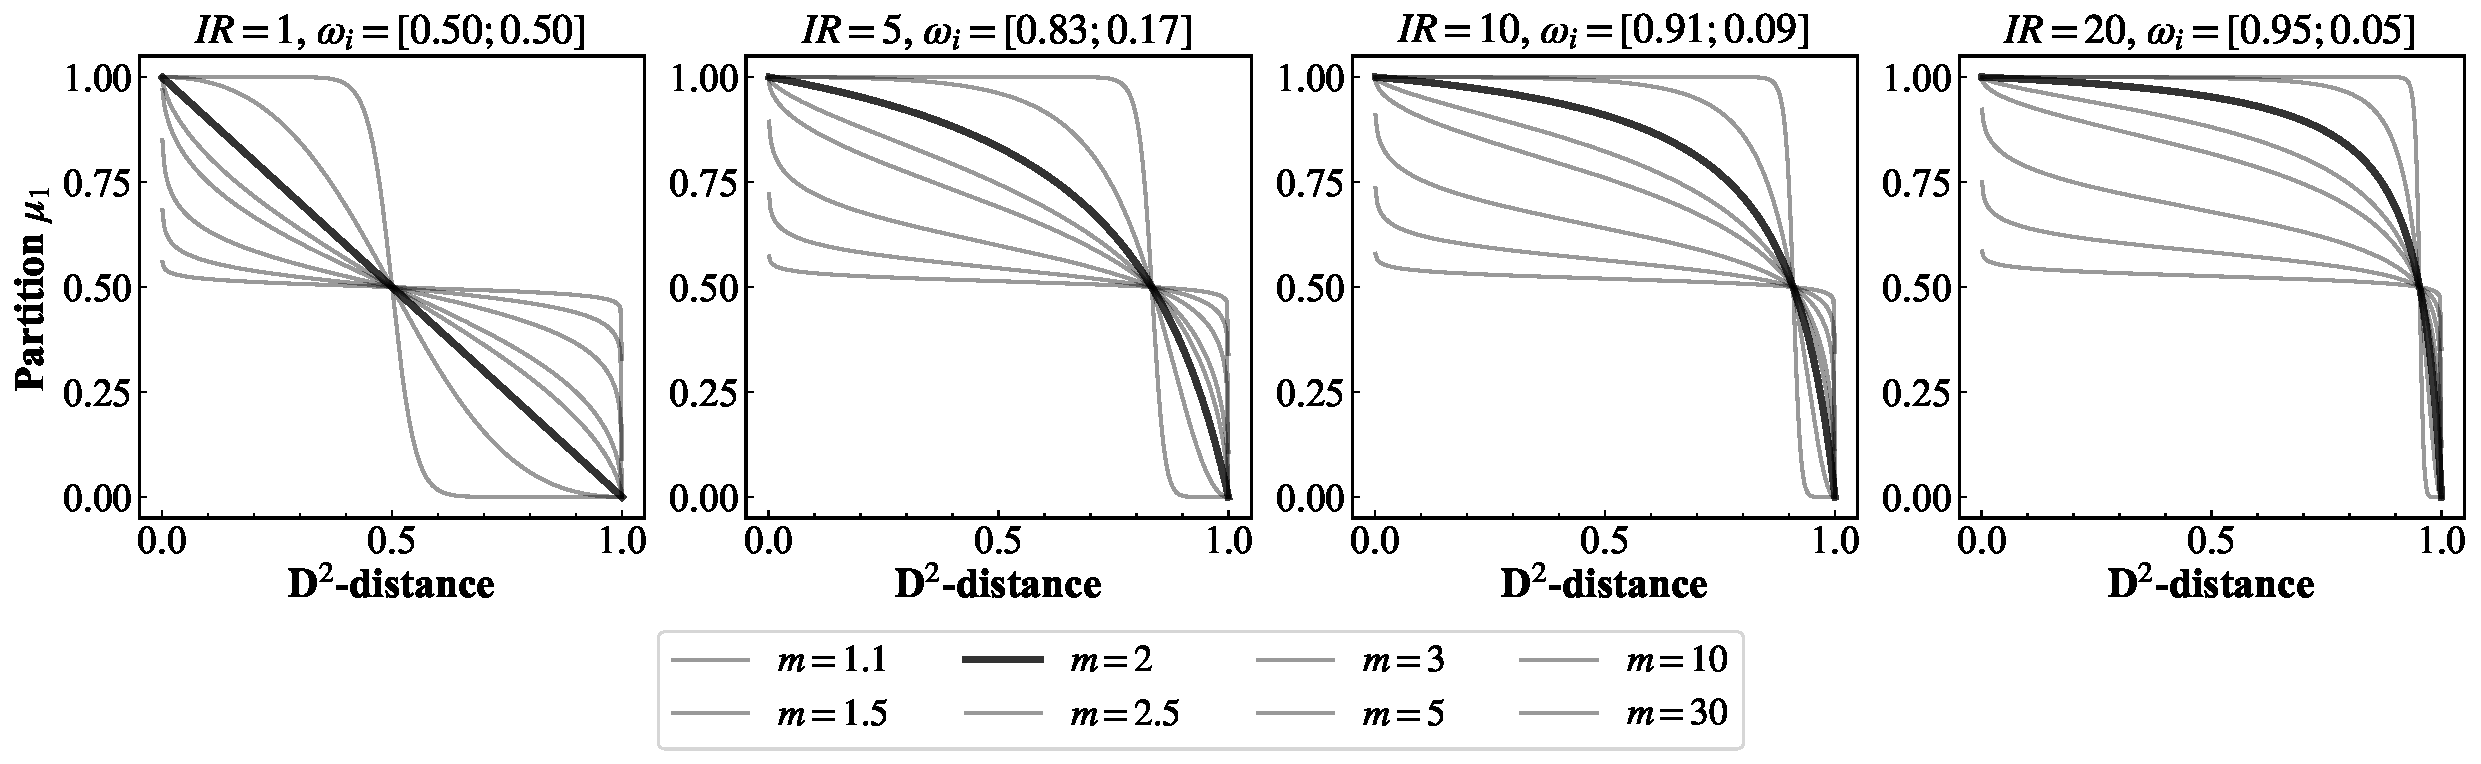
\includegraphics[width=\linewidth]{partition_m.pdf}
	\caption{Ảnh hưởng của tham số mờ $m$ trong EM-IFCM qua IR}\label{fig:ifcm}
\end{figure}


Hình~\ref{fig:ifcm} minh họa hành vi của IFCF khi $\delta=0$ trong môi trường ứng với các mức mất cân bằng khác nhau $IR=\{1\,; 5\,; 10\,; 20\}$, với trọng số tương ứng $\omega_i$ ở hai chùm. Ta thấy rằng với $IR=1$, các đường cong phân hoạch $\bm \mu_1$ đối xứng quanh khoảng cách $D^2$. Khi $IR$ tăng lên, chùm lớn chiếm ưu thế và các đường cong lệch rõ rệt về phía chùm lớn.  Ngoài ra, sự thay đổi của tham số mờ $ m $ từ $1,1$ đến $10,0$ cho thấy vai trò của nó trong việc kiểm soát độ mờ. Rõ ràng, các giá trị thấp hơn làm sắc nét ranh giới, trong khi các giá trị cao hơn tạo ra sự chuyển tiếp mềm hơn. Tóm lại, Thuật toán~\ref{alg:IFCF} mô tả cách thực hiện thuật toán IFCF.

%\begin{figure}[H]
%	\centering
%	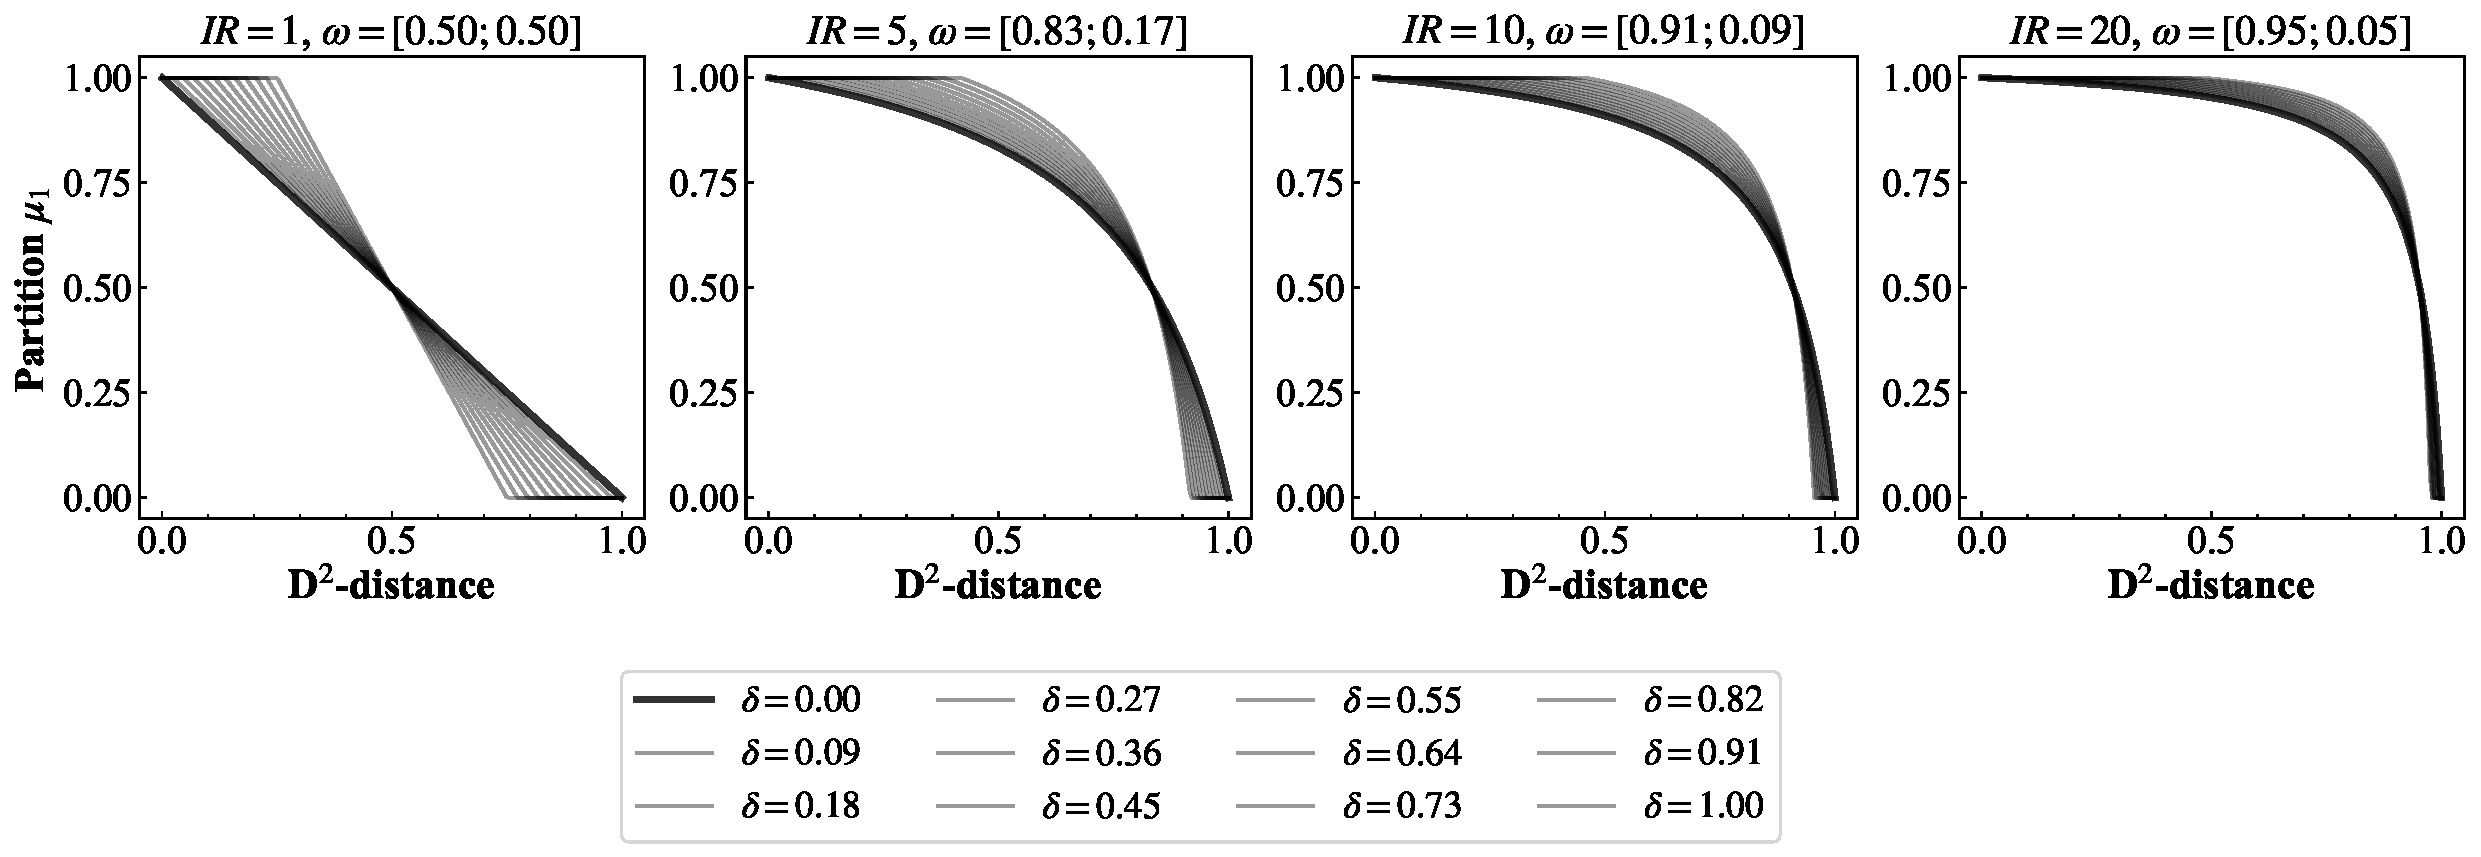
\includegraphics[width=\linewidth]{partition_delta.pdf}
%	\caption{Ảnh hưởng của tham số hiệu chỉnh biên $\delta$ trong IFCM qua IR}\label{fig:emifcm}
%\end{figure}
%
%Ngược lại, Hình~\ref{fig:emifcm} cho thấy tác động của tham số hiệu chỉnh biên $\delta$ trong IFCF khi cố định $m=2$. Khi $\delta>0$, thành phần hiệu chỉnh biên làm thay đổi đường phân vùng cong mạnh lên phía trên để giữa phân vùng của chùm nhỏ cao hơn, giúp duy trì giá trị phân vùng chùm nhỏ không bị suy giảm quá nhanh khi $IR$ lớn.





















\subsection{Tham số đánh giá chất lượng}

Đánh giá phân tích chùm cho biết độ hiệu quả thực thi của thuật toán bao gồm độ chính xác và độ phù hợp với thực tế. Các chỉ số đánh giá hiệu suất chùm (CVI) được sử dụng để đánh giá mối quan hệ giữa các thuộc tính của chùm đã hình thành bao gồm tính kết nối, tính gắn kết, tính đối xứng và tính tách biệt \cite{ikotun2025cluster}. Đánh giá kết quả phân tích chùm diễn ra trong hai trường hợp: đánh giá bên trong và bên ngoài. Tiêu chí đánh giá ngoài cung cấp độ chính xác giữa nhãn thực tế và nhãn kết quả của phân tích chùm trong các ví dụ mô phỏng. Nhưng trong thực tế, ta không có thông tin chính xác của nhãn nên phải đánh giá nội bộ. Đánh giá nội bộ cung cấp độ phù hợp của các chùm trong dữ liệu chưa được gán nhãn.

\subsubsection{a.\quad Đánh giá bên trong}

\begin{description}
	\item[Chỉ số Silhouette] Chỉ số Silhouette $S=\mathtt{mean}(s(f_j))$ đo mức độ phù hợp của một hàm mật độ \(f_j\) với chùm mà nó được gán nhãn, so với chùm gần nhất khác, trong đó
	$
	s(f_j) = \frac{b(f_j) - a(f_j)}{\max \{ a(f_j), b(f_j) \}},
	$
	với \( a(f_j) = \frac{1}{\#c_k-1} \sum\limits_{\substack{f \in c_k \\ f \ne f_j}} D(f_j, f) \) là khoảng cách trung bình giữa \(f_j\) và tất cả các hàm mật độ khác trong chùm \(c_k\) chứa nó, và \( b(f_j) = \min\limits_{l \ne k} \frac{1}{\#c_l} \sum\limits_{f \in c_l} D(f_j, f) \) là khoảng cách trung bình giữa \(f_j\) và các hàm mật độ trong chùm gần nhất \(c_l\) với \( l \ne k \).
	\item[Chỉ số Dunn] Chỉ số Dunn đánh giá mức độ tách biệt giữa các chùm, được định nghĩa bởi
	$
	D = \frac{\displaystyle \min_{k \ne l} \Delta_{\min}(c_k, c_l)}
	{\displaystyle \max_{m} \Delta(c_m)},
	$
	trong đó, \( \Delta_{\min}(c_k, c_l) = \min\limits_{\substack{f \in c_k \\ g \in c_l}} D(f, g) \) là liên kết nhỏ nhất giữa hai chùm \(c_k\) và \(c_l\), và \( \Delta(c_m) = \max\limits_{f, g \in c_m} D(f, g) \) là đường kính lớn nhất của chùm \(c_m\).
	\item[Chỉ số Davies--Bouldin] Chỉ số Davies--Bouldin đo mức độ tương đồng giữa các chùm, được định nghĩa bởi
	$
	DI = \frac{1}{k} \sum_{k=1}^{K} \max_{l \ne k}
	\left\{ \frac{S_k + S_l}{D(\theta_k, \theta_l)} \right\},
	$
	trong đó, \( S_k = \frac{1}{|c_k|} \sum\limits_{f \in c_k} D(f, \theta_k) \) là độ phân tán trung bình của chùm \(c_k\), \( \theta_k \) là trọng tâm của chùm \(c_k\), \( D(\theta_k, \theta_l) \) là khoảng cách giữa hai trọng tâm \(\theta_k\) và \(\theta_l\) và \(k\) là số chùm.
	
\end{description}

Chỉ số Silhouette và Dunn có giá trị càng nhỏ, kết quả phân tích chùm càng tốt. Ngược lại, chỉ số Davies--Bouldin càng nhỏ càng tốt. Ngoài ra, hệ số tương tự chùm (Bảng~\ref{tab:chumham}) cũng đã được xem như một chỉ số bên ngoài để đánh giá sự tương tự của hai chùm hàm mật độ \cite{vovan2018similar}.

\begin{figure}[H]
	\centering
	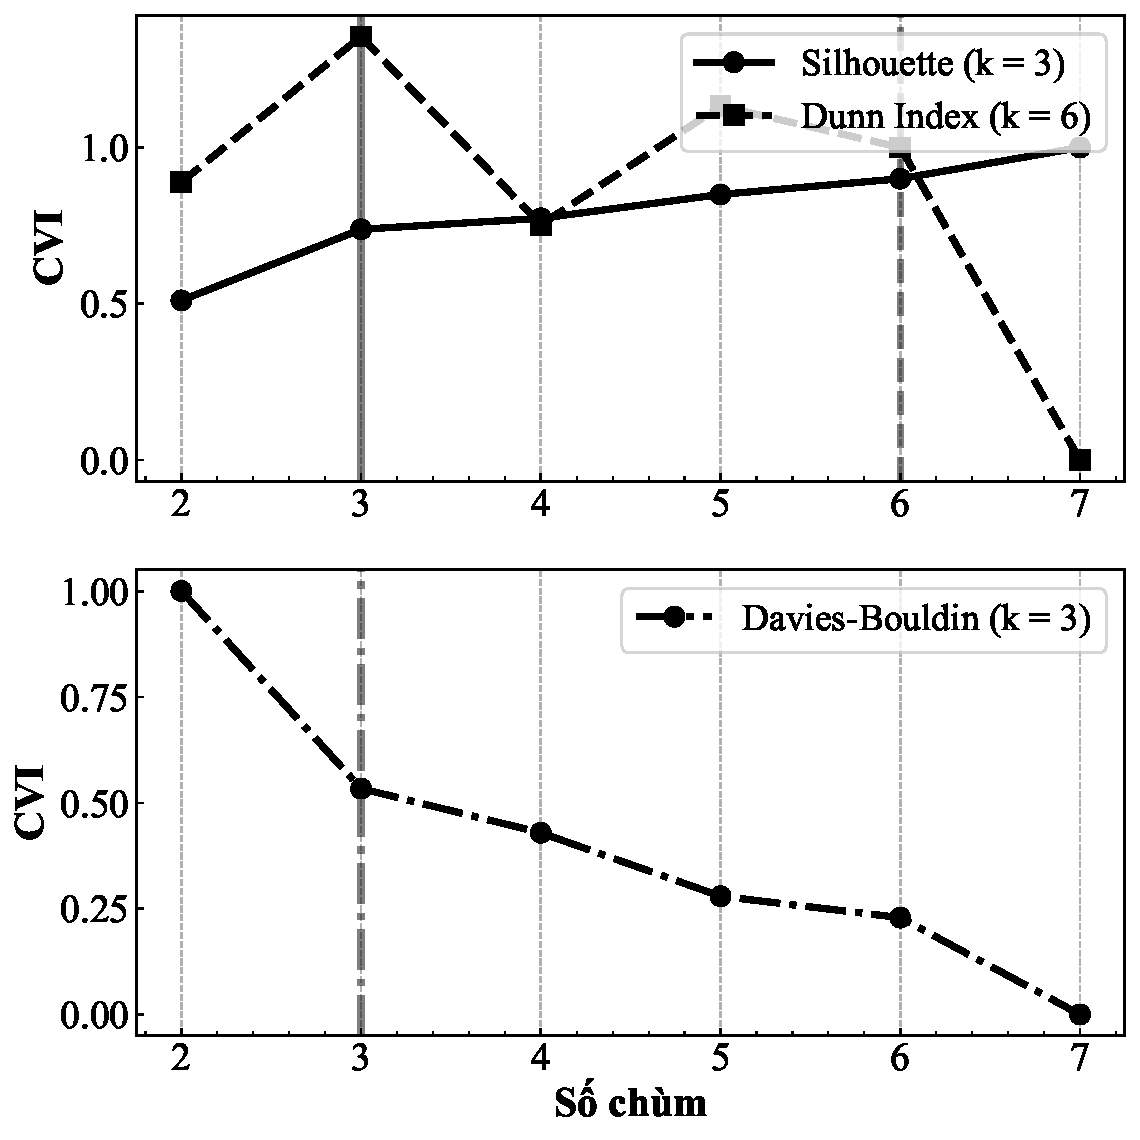
\includegraphics[width=.5\linewidth]{C2_k_best_FCF.pdf}
	\begin{flushleft}
		\footnotesize\it
		Chú thích: Hình ở trên thể hiện chỉ số Silhouette và Dunn vì chúng càng lớn càng tốt. Ngược lại, chỉ số DBI càng nhỏ càng tốt. Điểm khuỷ tay là điểm mà ở đó độ dốc giữa hai dãy chùm bất kỳ đạt cực đại. Ở đây, ta thấy chỉ số Silhouette và DBI đều đề xuất $k$-chùm tối ưu là $k=3$. Trong khi đó, chỉ~số Dunn cho kết quả $k=6$. 
	\end{flushleft}
	\caption[Một số chỉ số đánh giá và số chùm tối ưu]{Một số chỉ số đánh giá và số chùm tối ưu được đề xuất từ phương pháp khuỷu tay với dữ liệu hàm mật độ ở Ví dụ~\ref{VD:thubac}.}
	\label{fig:c1kbestfcf}
\end{figure}



\subsubsection{b.\quad Đánh giá bên ngoài}

Đánh giá bên ngoài được sử dụng khi có nhãn thực tế \(\mathcal{P} = \{\mathcal{F}_1\,; \ldots\,; \mathcal{F}_R\}\) của tập hàm mật độ \(\mathcal{F} = \{f_1\,; \ldots\,; f_n\}\) và kết quả phân chùm \(\mathcal{G} = \{\mathcal{G}_1\,; \ldots\,; \mathcal{G}_K\}\).  
Xét các cặp \((f_i\,; f_j)\), ta có các trường hợp
\[
\begin{aligned}
	a &= \#\{(f_i\,;f_j)\,|\, f_i\,;f_j \in \mathcal{F}_r \cap \mathcal{G}_k\}, \\
	b &= \#\{(f_i\,;f_j)\,|\, f_i\,;f_j \in \mathcal{F}_r\,; f_i \in \mathcal{G}_k\,; f_j \in \mathcal{G}_l\,; k \neq l\}\,; \\
	c &= \#\{(f_i\,;f_j)\,|\, f_i\,;f_j \in \mathcal{G}_k\,; f_i \in \mathcal{F}_r\,; f_j \in \mathcal{F}_s\,; r \neq s\}\,; \\
	d &= \#\{(f_i\,;f_j)\,|\, f_i \in \mathcal{F}_r \cap \mathcal{G}_k\,; f_j \in \mathcal{F}_s \cap \mathcal{G}_l\,; r \neq s\,; k \neq l\}.
\end{aligned}
\]

\begin{table}[H]
	\centering
	\scriptsize
	\caption{Các chỉ số đánh giá độ tương đồng giữa hai phân hoạch}
	\begin{tabular*}{\textwidth}{@{\extracolsep\fill}lp{4cm}p{11cm}@{\extracolsep\fill}}
		\toprule
		\textbf{Chỉ số} & \textbf{Công thức} & \textbf{Ý nghĩa} \\
		\midrule
		Rand Index (RI) &
		\(RI = \dfrac{a+d}{a+b+c+d}\) &
		 Đo mức độ tương đồng/chính xác của \(\mathcal{P}\) theo \(\mathcal{G}\)\\[2mm]
		Adjusted Rand Index (ARI) &
		\(ARI = \dfrac{RI - \mathbb{E}(RI)}{\max(RI) - \mathbb{E}(RI)}\) &
		Loại bỏ trùng khớp ngẫu nhiên; giá trị tối đa là 1.\\[2mm]
		Fowlkes–Mallows Index (FMI) &
		\(FMI = \sqrt{\dfrac{a}{a+b}\cdot\dfrac{a}{a+c}}\) &
		Đo lường cặp đúng/sai dựa trên precision và recall.\\[2mm]
		Jaccard Index (J) &
		\(J = \dfrac{a}{a+b+c}\) &
		Tỷ lệ cặp cùng chùm trên tổng số cặp liên quan.\\[2mm]
		Normalized Mutual Infomation (NMI) &
		\(NMI = \dfrac{2\,I(\mathcal P,\mathcal G)}{H(\mathcal P)+H(\mathcal G)}\) &
		Đo mức độ phụ thuộc thông tin giữa hai phân hoạch.\\
		\bottomrule
	\end{tabular*}
	\begin{flushleft}\it\footnotesize
		Trong đó, \( p_i = \frac{\#\mathcal{F}_i}{n},\, p_j = \frac{\#\mathcal{G}_j}{n},\, p_{ij} = \frac{\#(\mathcal{F}_i \cap \mathcal{G}_j)}{n}, \) ta có, $I(\mathcal{P},\mathcal{Q}) = \sum_{i,j} p_{ij} \log \frac{p_{ij}}{p_i p_j}$, với $H(\mathcal{P}) = - \sum_i p_i \log p_i \,;
		H(\mathcal{Q}) = - \sum_j p_j \log p_j.$
	\end{flushleft}
\end{table}





\subsection{Ví dụ minh hoạ}



Để khảo sát hành vi của thuật toán được đề xuất trong các bài toán chuẩn, trước tiên luận văn này tạo dữ liệu tổng hợp qua hai ví dụ Gauss hai chùm và Gauss lệch ba chùm.
\subsubsection{a.\qquad Dữ liệu mô phỏng}



\vdu{[Hàm Gauss, hai chùm]\label{vdu:gauss1} 
	Giả sử dữ liệu được tạo theo công thức tổng quát về kỳ vọng và độ lệch chuẩn của mỗi chùm, cụ thể như sau.
	\begin{align*}
		\begin{array}{clll}
			\text{Chùm } 1: & f(x\,\vert \,\mu\,;\sigma^2)\sim \mathcal{N}(\mu_1\,;\sigma_1^2)\,; 
			\text{với } \mu_1 \sim \mathcal{N}(-5,0\,;1,0)\,;\;\sigma_1 = 2,0,\\
			\text{Chùm } 2: & f(x\,\vert \,\mu\,;\sigma^2)\sim \mathcal{N}(\mu_2\,;\sigma_2^2)\,; 
			\text{với } \mu_2 \sim \mathcal{N}(5,0\,;1,0)\,;\;\sigma_2 = 4,0.
		\end{array}
	\end{align*}

\begin{figure}[H]
	\centering
	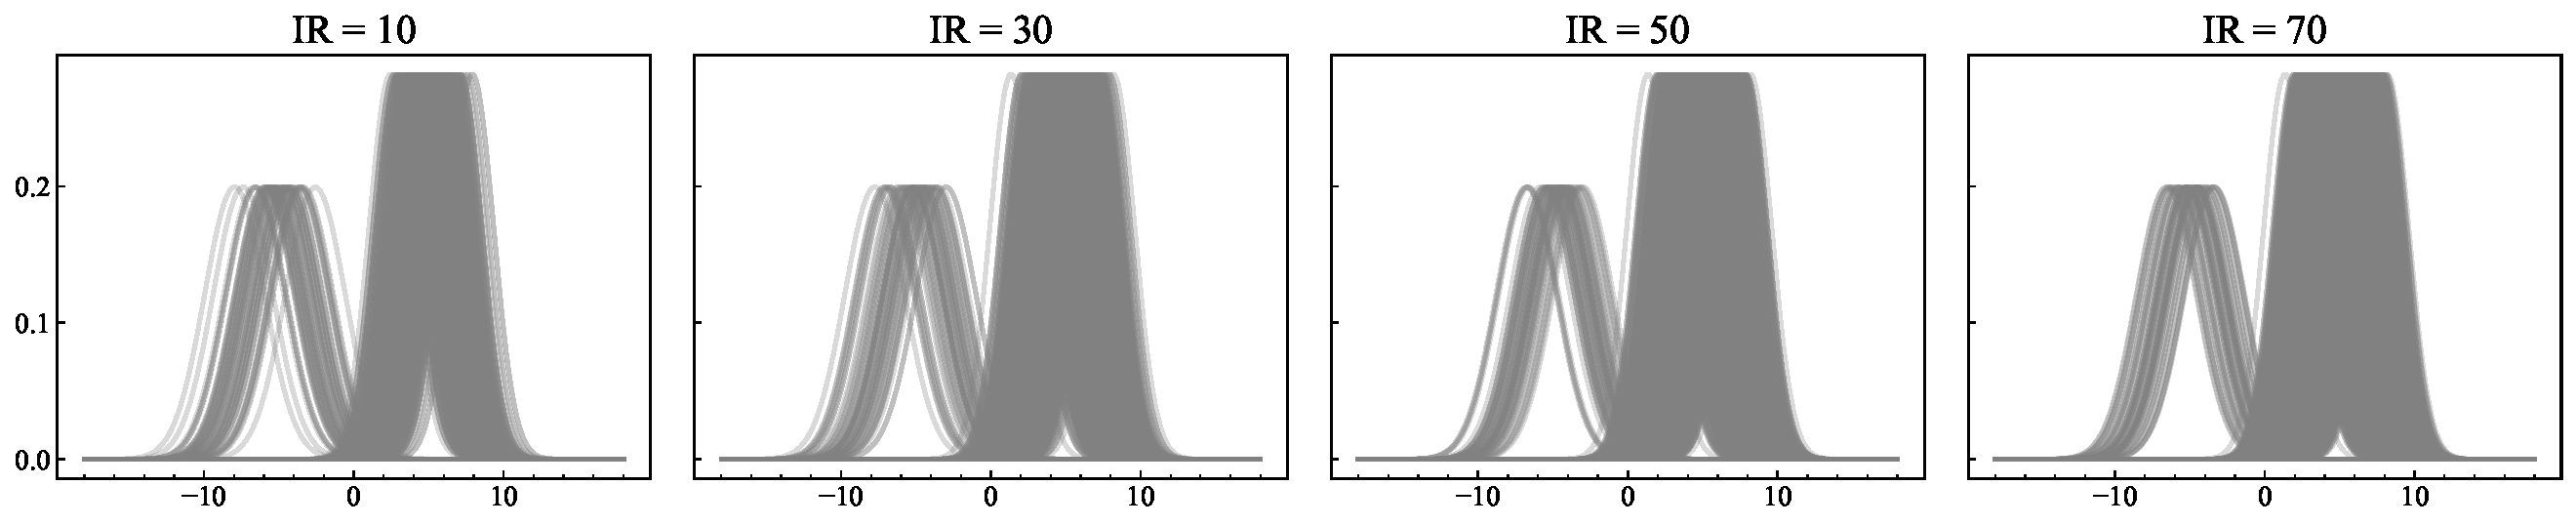
\includegraphics[width=\linewidth]{pdf_bandau}
	\caption{Dữ liệu tại Ví dụ \ref{vdu:gauss1}}\label{fig:vdu:gauss1}
\end{figure}

	Luận văn mô phỏng dữ liệu hàm mật độ Gauss trên tập số thực với hai chùm được giả định trước. Vai trò chính của dữ liệu nhân tạo này là đánh giá độ ổn định của thuật toán trong các kịch bản mất cân bằng nghiêm trọng khi $IR$ thay đổi từ $10$ đến $50$. $IR$ càng lớn thì sự chênh lệch giữa chùm $1$ và $2$ càng cao. Hình~\ref{fig:vdu:gauss1} thể hiện rõ tác động của $IR$ lên phân bố dữ liệu. Khi $IR$ tăng ($1:10$, $1:30$, và $1:50$), chùm lớn hơn trở nên dày đặc hơn, trong khi chùm nhỏ giữ nguyên kích thước.}








%\vdu{[Hàm Gauss-lệch, ba chùm]  Giả sử phân phối lệch-Gauss từ \url{http://azzalini.stat.unipd.it/SN/}. Hàm mật độ của phân phối lệch–Gauss được định nghĩa như sau.
%\begin{align*}
%	f(x \,\vert \, \xi\,; \sigma\,; \lambda)=\frac{2}{\lambda}\phi\left(\frac{x-\xi}{\sigma}\right)\Phi\left(\lambda\frac{x-\xi}{\sigma}\right),
%\end{align*}
%trong đó $\phi(\cdot)$ và $\Phi(\cdot)$ lần lượt là hàm mật độ chuẩn và hàm phân phối tích lũy chuẩn. Tham số $\xi$ là vị trí của kỳ vọng, $\sigma$ là độ lệch chuẩn, và $\lambda$ điều khiển độ lệch (skewness). Trong khung nghiên cứu này, tham số vị trí $\xi_i$ được lấy mẫu từ các phân phối chuẩn $\mathcal{N}(0\,;0.2)$, $\mathcal{N}(2\,;0.2)$ và $\mathcal{N}(-2\,;0.2)$ tương ứng cho chùm, $1$, $2$ và $3$. Các tham số độ lệch-Gauss được đặt là $\sigma_i=[0\,; 10\,; -10]$, trong khi các tham số lệch được xác định là $\lambda_i=[1\,; 2\,; 2]$, nhằm tạo ra sự bất đối xứng giữa các chùm.
%
%
%Trong ví dụ này, luận văn mở rộng Ví dụ \ref{vdu:gauss1} sang ba chùm nhằm tăng độ phức tạp và tạo sự khác biệt lớn hơn. Các hàm mật độ của ba chùm này được minh họa trong Hình~\ref{fig:EX3_main}, với các tỷ lệ $IR$ khác nhau: (a) $1:10:10$, (b) $1:50:50$, và (c) $1:100:100$. 


%\begin{figure}[H]
%	\centering
%	\begin{subfigure}[b]{0.32\linewidth} 
%		\centering
%		\includegraphics[width=\textwidth]{Fig/EX3_IR_10.eps}
%		\caption{IR: $1:10:10$}
%	\end{subfigure}
%	\begin{subfigure}[b]{0.32\linewidth} 
%		\centering
%		\includegraphics[width=\textwidth]{Fig/EX3_IR_50.eps}
%		\caption{IR: $1:50:50$}
%	\end{subfigure}
%	\begin{subfigure}[b]{0.32\linewidth} 
%		\centering
%		\includegraphics[width=\textwidth]{Fig/EX3_IR_100.eps}
%		\caption{IR: $1:100:100$}
%	\end{subfigure}
%	\caption{Ba chùm hàm mật độ trong Ví dụ 2.}
%	\label{fig:EX3_main}
%\end{figure}

%}









\subsubsection{b.\qquad Kết quả các loại khoảng cách}

Các thuật toán phân chùm hoạt động với nhiều công thức đo khác nhau, bao gồm khoảng cách $\mathcal{L}_2$,  Hellinger, Bhattacharyya, và Wasserstein-2 (Bảng~\ref{tab1:KC_PDF}). Để bảo đảm tính công bằng, số chùm $c=2$, tham số mờ $m=2,0$, sai số hội tụ $\varepsilon=10^{-12}$, số vòng lặp tối đa $T_{\max}=200$ và phương pháp khởi tạo được cố định là $k$-mean++\index{$k$-mean++}. 


\begin{table}[H]
	\centering
	\scriptsize
	\caption{So sánh các loại khoảng cách với các mức IR}
	\begin{tabular*}{\textwidth}{@{\extracolsep\fill}lcccccc@{\extracolsep\fill}}
		\toprule
		\textbf{Khoảng cách} & \textbf{IR} & Sil & DI & DBI & ARI & NMI \\
		\midrule
		\multirow{3}{*}{BC}
		& 10 & 0.65$\pm$0.00 & 0.90$\pm$0.00 & 0.49$\pm$0.00 & 1.00$\pm$0.00 & 1.00$\pm$0.00 \\
		& 30 & 0.62$\pm$0.00 & 0.87$\pm$0.00 & 0.49$\pm$0.00 & 1.00$\pm$0.00 & 1.00$\pm$0.00 \\
		& 50 & 0.62$\pm$0.00 & 0.83$\pm$0.00 & 0.54$\pm$0.00 & 1.00$\pm$0.00 & 1.00$\pm$0.00 \\
		\midrule
		\multirow{3}{*}{Hellinger}
		& 10 & 0.65$\pm$0.00 & 0.90$\pm$0.00 & 0.49$\pm$0.00 & 1.00$\pm$0.00 & 1.00$\pm$0.00 \\
		& 30 & 0.62$\pm$0.00 & 0.87$\pm$0.00 & 0.49$\pm$0.00 & 1.00$\pm$0.00 & 1.00$\pm$0.00 \\
		& 50 & 0.62$\pm$0.00 & 0.83$\pm$0.00 & 0.54$\pm$0.00 & 1.00$\pm$0.00 & 1.00$\pm$0.00 \\
		\midrule
		\multirow{3}{*}{$\mathcal{L}_2$}
		& 10 & 0.65$\pm$0.00 & 0.90$\pm$0.00 & 0.49$\pm$0.00 & 1.00$\pm$0.00 & 1.00$\pm$0.00 \\
		& 30 & 0.62$\pm$0.00 & 0.87$\pm$0.00 & 0.49$\pm$0.00 & 1.00$\pm$0.00 & 1.00$\pm$0.00 \\
		& 50 & 0.62$\pm$0.00 & 0.83$\pm$0.00 & 0.54$\pm$0.00 & 1.00$\pm$0.00 & 1.00$\pm$0.00 \\
		\midrule
		\multirow{3}{*}{W2}
		& 10 & 0.65$\pm$0.00 & 0.90$\pm$0.00 & 0.49$\pm$0.00 & 1.00$\pm$0.00 & 1.00$\pm$0.00 \\
		& 30 & 0.62$\pm$0.00 & 0.87$\pm$0.00 & 0.49$\pm$0.00 & 1.00$\pm$0.00 & 1.00$\pm$0.00 \\
		& 50 & 0.62$\pm$0.00 & 0.83$\pm$0.00 & 0.54$\pm$0.00 & 1.00$\pm$0.00 & 1.00$\pm$0.00 \\
		\bottomrule
	\end{tabular*}
\end{table}












\subsubsection{c.\qquad  Kết quả các tham số mờ}




\begin{table}[H]
	\centering
	\scriptsize
	\caption{So sánh các mức Fuzziness với các giá trị IR}
	\begin{tabular*}{\textwidth}{@{\extracolsep\fill}lcccccc@{\extracolsep\fill}}
		\toprule
		\textbf{Tham số mờ} & \textbf{IR} & Sil & DI & DBI & ARI & NMI \\
		\midrule
		\multirow{3}{*}{1.1}
		& 10 & 0.65$\pm$0.00 & 0.90$\pm$0.00 & 0.49$\pm$0.00 & 1.00$\pm$0.00 & 1.00$\pm$0.00 \\
		& 30 & 0.62$\pm$0.00 & 0.87$\pm$0.00 & 0.49$\pm$0.00 & 1.00$\pm$0.00 & 1.00$\pm$0.00 \\
		& 50 & 0.62$\pm$0.00 & 0.83$\pm$0.00 & 0.54$\pm$0.00 & 1.00$\pm$0.00 & 1.00$\pm$0.00 \\
		\midrule
		\multirow{3}{*}{1.5}
		& 10 & 0.65$\pm$0.00 & 0.90$\pm$0.00 & 0.49$\pm$0.00 & 1.00$\pm$0.00 & 1.00$\pm$0.00 \\
		& 30 & 0.62$\pm$0.00 & 0.87$\pm$0.00 & 0.49$\pm$0.00 & 1.00$\pm$0.00 & 1.00$\pm$0.00 \\
		& 50 & 0.62$\pm$0.00 & 0.83$\pm$0.00 & 0.54$\pm$0.00 & 1.00$\pm$0.00 & 1.00$\pm$0.00 \\
		\midrule
		\multirow{3}{*}{2.0}
		& 10 & 0.65$\pm$0.00 & 0.90$\pm$0.00 & 0.49$\pm$0.00 & 1.00$\pm$0.00 & 1.00$\pm$0.00 \\
		& 30 & 0.62$\pm$0.00 & 0.87$\pm$0.00 & 0.49$\pm$0.00 & 1.00$\pm$0.00 & 1.00$\pm$0.00 \\
		& 50 & 0.62$\pm$0.00 & 0.83$\pm$0.00 & 0.54$\pm$0.00 & 1.00$\pm$0.00 & 1.00$\pm$0.00 \\
		\midrule
		\multirow{3}{*}{2.5}
		& 10 & 0.65$\pm$0.00 & 0.90$\pm$0.00 & 0.49$\pm$0.00 & 1.00$\pm$0.00 & 1.00$\pm$0.00 \\
		& 30 & 0.62$\pm$0.00 & 0.87$\pm$0.00 & 0.49$\pm$0.00 & 1.00$\pm$0.00 & 1.00$\pm$0.00 \\
		& 50 & 0.62$\pm$0.00 & 0.83$\pm$0.00 & 0.54$\pm$0.00 & 1.00$\pm$0.00 & 1.00$\pm$0.00 \\
		\midrule
		\multirow{3}{*}{3.0}
		& 10 & 0.65$\pm$0.00 & 0.90$\pm$0.00 & 0.49$\pm$0.00 & 1.00$\pm$0.00 & 1.00$\pm$0.00 \\
		& 30 & 0.62$\pm$0.00 & 0.87$\pm$0.00 & 0.49$\pm$0.00 & 1.00$\pm$0.00 & 1.00$\pm$0.00 \\
		& 50 & 0.62$\pm$0.00 & 0.83$\pm$0.00 & 0.54$\pm$0.00 & 1.00$\pm$0.00 & 1.00$\pm$0.00 \\
		\midrule
		\multirow{3}{*}{5.0}
		& 10 & 0.65$\pm$0.00 & 0.90$\pm$0.00 & 0.49$\pm$0.00 & 1.00$\pm$0.00 & 1.00$\pm$0.00 \\
		& 30 & 0.62$\pm$0.00 & 0.87$\pm$0.00 & 0.49$\pm$0.00 & 1.00$\pm$0.00 & 1.00$\pm$0.00 \\
		& 50 & 0.62$\pm$0.00 & 0.83$\pm$0.00 & 0.54$\pm$0.00 & 1.00$\pm$0.00 & 1.00$\pm$0.00 \\
		\midrule
		\multirow{3}{*}{10.0}
		& 10 & 0.65$\pm$0.00 & 0.90$\pm$0.00 & 0.49$\pm$0.00 & 1.00$\pm$0.00 & 1.00$\pm$0.00 \\
		& 30 & 0.62$\pm$0.00 & 0.87$\pm$0.00 & 0.49$\pm$0.00 & 1.00$\pm$0.00 & 1.00$\pm$0.00 \\
		& 50 & 0.62$\pm$0.00 & 0.83$\pm$0.00 & 0.54$\pm$0.00 & 1.00$\pm$0.00 & 1.00$\pm$0.00 \\
		\bottomrule
	\end{tabular*}
\end{table}









\subsubsection{d.\qquad  Kết quả các loại phân tích chùm}


\begin{table}[H]
	\centering
	\scriptsize
	\caption{So sánh các tham số mờ $m$ với các mức IR}
	\begin{tabular*}{\textwidth}{@{\extracolsep\fill}llccc@{\extracolsep\fill}}
		\toprule
		\textbf{Thuật toán} & \textbf{Chỉ số đánh giá} & $IR=10$ & $IR=30$ & $IR=50$ \\
		\midrule
		\multirow{5}{*}{Thuật toán IFCF (đề xuất)}
		& Sil  & -- & -- & -- \\
		& DI   & -- & -- & -- \\
		& DBI  & -- & -- & -- \\
		& ARI  & -- & -- & --  \\
		& NMI  & -- & -- & -- \\
		\midrule
		\multirow{5}{*}{Thuật toán FCF \cite{nguyentrang2017fuzzy}}
		& Sil  & -- & -- & -- \\
		& DI   & -- & -- & -- \\
		& DBI  & -- & -- & -- \\
		& ARI  & -- & -- & --  \\
		& NMI  & -- & -- & -- \\
		\midrule
		\multirow{5}{*}{Thuật toán KCF \cite{pham2019new}}
		& Sil  & -- & -- & -- \\
		& DI   & -- & -- & -- \\
		& DBI  & -- & -- & -- \\
		& ARI  & -- & -- & --  \\
		& NMI  & -- & -- & -- \\
		\bottomrule
	\end{tabular*}
\end{table}





















\subsection{Phương pháp phân loại hàm mật độ xác suất}


Phương pháp phân loại là một nhánh của nhận dạng có giám sát, phát triển với mục tiêu thành lập quy tắc quy nạp có chức năng phân tách được các lớp quan tâm với sai lầm thực nghiệm tối tiểu.  Các quy luật đánh giá có bệnh B hay không dựa vào những dữ liệu cho trước chính là thực hiện bài toán phân loại. Hay phân biệt được hữu hạn các biểu cảm khuôn mặt dựa vào hình ảnh cũng phải thực hiện bài toán phân loại. Đầu ra của mô hình phân loại là ước tính hoặc dự đoán hữu hạn các nhãn cho trước (không đo được) với dữ liệu mới chưa được mô hình hóa \cite{Fillmore-Patrick_2025}. 

%Trong bài toán phân loại, ta giả sử tồn tại một không gian đầu vào $\mathcal{F}$ và tập nhãn rời rạc ${Y} = \{1, 2, \dots, C\}$. Cặp dữ liệu $(f, y)$ là biến ngẫu nhiên có phân phối chung $P_{\mathcal{F},Y}$ trên $\mathcal{F} \times {Y}$.  Mục tiêu của bài toán là tìm một ánh xạ phân loại $h : \mathcal{F} \to {Y}$ thuộc không gian giả thuyết $\mathcal{H}$ sao cho tối tiểu hóa giá trị kỳ vọng của hàm mất mát\index{hàm mất mát (loss function)} $\ell : {Y} \times {Y} \to \mathbb{R}_{\ge 0}$, tức là $
%	h^* = \arg\min_{h \in \mathcal{H}} \mathbb{E}{(f,y)\sim P_{\mathcal{F},Y}} \left[\ell(h(f), y)\right].$ Tuy nhiên, do phân phối thực $P_{\mathcal{F}\,;{Y}}$ là chưa biết, ta cần tiếp cận qua một tập huấn luyện $\mathcal{D}_n = \{(f_1, y_1), \ldots, (f_n, y_n)\} \subset \mathcal{F} \times {Y}$. Vì vậy, ta giải bài toán 
%$$
%\hat{h}_n = \arg\min{h \in \mathcal{H}} \frac{1}{n} \sum_{j=1}^n \ell(h(f_j), y_j).
%$$


Phương pháp phân loại cho hàm mật độ xác suất là một bài toán mới mẻ nên còn nhiều thách thức lớn cả bề sâu và bề rộng. Nhìn chung cho đến nay, hai phương pháp chính để phân loại là từ hai góc nhìn. Xem hàm mật độ là một véc-tơ hữu hạn chiều hay hàm vô hạn chiều. 


\begin{table}[H]
	\centering
	\scriptsize
	\begin{tabular*}{\textwidth}{@{\extracolsep\fill}lp{4cm}p{11cm}@{\extracolsep\fill}}
		\toprule
		\textbf{Năm} & \textbf{Tác giả} & \textbf{Mô tả phương pháp} \\
		\midrule
		2004 & Bi Jinbo \& Zhang Tong \cite{bi2004support} & Máy véc-tơ hỗ trợ với bất định đầu vào: giả sử nhiễu cộng $\Delta x_i$ bị chặn $|\Delta x_i|\le \delta_i$. Giải biên tồi nhất cho ra hinge-loss hiệu chỉnh; có thể kernel hoá. \\
		2009 & Ren Jiangtao \textit{et al.} \cite{ren2009naive} & Naive Bayes cho dữ liệu bất định: ước lượng mật độ điều kiện lớp bằng kỳ vọng kernel trên hàm mật độ; ba biến thể AVG/SBC/FBC (FBC thường tốt nhất). \\
		2009 & Tsang Smith \textit{et al.} \cite{tsang2009decision} & Cây quyết định, chia nút bằng entropy kỳ vọng từ các bộ ba phân số khi tách ngưỡng. \\
		2023 & Tai Vo-Van, Hieu Nguyen Thi Kim \& Dinh Pham-Toan \cite{vovan2023multi} & \\
		2023 & Pavlů \textit{et al.} \cite{pavluu2023classification} & Nhúng hàm mật độ vào không gian Bayes, triển khai logistic hàm mật độ cho không gian này \\
		2024 & Thu-Anh Nguyen-Tran, An Thien Ngoc Nguyen \& Dinh Pham-Toan\cite{tran2025novel}&\\
		2025 & Tai Vo-Van \& Dinh Pham-Toan \cite{vo2024supervised} & Học đa lớp cho dữ liệu hàm mật độ bằng phương pháp Bayes cải tiến\\
		2025 & Tai Vo-Van \cite{vovan2025classifying} & Cải thiện độ chính xác trong phân loại dữ liệu hình ảnh đa kênh màu bằng Bayes cải tiến \\
		2025 & Tai Vo-Van \cite{vo2025developing} &  Phát triển phương pháp phân loại Bayes cải tiến bằng khoảng cách tương tự chùm, \\
		\bottomrule
	\end{tabular*}
	\begin{flushleft}\it\footnotesize
		
	\end{flushleft}
	\caption{Tổng quan phương pháp phân loại cho hàm mật độ xác suất}
	\label{tab:pdf_classification_summary}
\end{table}






\section{Giới thiệu bài toán phân loại cho dữ liệu mất cân bằng}





\subsection{Thuật toán}

Thuật toán này gồm hai giai đoạn: trích xuất đặc trưng ảnh thành hàm mật độ xác suất, sau đó thiết lập nguyên tắc phân loại dựa vào Bayes. Giả sử có $c$ lớp $c_i$, trong đó nhóm $c_i$ chứa $n_j$ đối tượng hàm mật độ. Phân loại một hàm mật độ mới  $h(x)$ vào nhóm $c_i$ bằng quy tắc Bayes. Gán một phần tử mới vào một lớp nếu nó có xác suất hậu nghiệm đối với lớp đó là cao nhất, tức là $c_i = \arg \max_{1 \leq i \leq c} \left\{\mu_i \cdot D(h, \theta_i)\right\}.$ Trong đó, xác suất tiên nghiệm được tính bằng Thuật toán~\ref{alg:IFCF}, khoảng cách $D$ được chuẩn hóa trong khoảng $[0\,;1]$.









\subsection{Tham số đánh giá chất lượng}

Đối với thuật toán phân loại, ta đánh giá kết quả dự đoán thông qua độ chính xác của mô hình trên tập dữ liệu chưa được huấn luyện. Kết quả phân loại thường được tóm tắt trong ma trận nhầm lẫn\index{ma trận nhầm lẫn (confusion matrix)}, thể hiện số lượng dự đoán đúng và sai của mô hình. Giả sử ta có một bài toán phân loại nhị phân với hai lớp \(\{\,\text{Dương tính}\,; \text{Âm tính}\,\}\). Ma trận nhầm lẫn có dạng

{\footnotesize\begin{center}
\begin{tabular}{c|cc}
	\toprule
	& \text{Dự đoán dương tính} & \text{Dự đoán âm tính} \\
	\midrule
	\text{Thực tế dương tính} & \text{Dương tính thật } ($\#TP$) & \text{Âm tính giả } ($\#FN$) \\
	\text{Thực tế âm tính} & \text{Dương tính giả } ($\#FP$) & \text{Âm tính thật } ($\#TN$) \\
	\bottomrule
\end{tabular}
	\end{center}
}

Ví dụ khi ta phân loại các ca có bệnh B hoặc không có bệnh B, $\#TP$ thể hiện số lượng dự đoán đúng kết luận có bệnh B; $\#FP$ là số dự đoán đúng không bệnh. Ngược lại $\#FN$ là số dự đoán kết luận không bệnh, nhưng thực tế là có; và $\#FP$ là số dự đoán kết luận có bệnh B, nhưng thực tế là không.
Từ ma trận nhầm lẫn, ta định nghĩa các chỉ số phổ biến khác. Các chỉ số trong Bảng~\ref{tab:index_phanloai} cung cấp cơ sở định lượng cho việc đánh giá hiệu năng mô hình, 

\begin{table}[H]
	\centering\scriptsize
	\caption{Mô tả các chỉ số đánh giá phân loại}\label{tab:index_phanloai}
	\begin{tabular*}{\columnwidth}{@{\extracolsep\fill}lllc@{\extracolsep\fill}} 
		\toprule
		\textbf{Chỉ số} & \textbf{Công thức}                                                                         & \textbf{Ý nghĩa}                             & \textbf{Phạm vi} \\ \midrule
		Độ chính xác (ACC) & $\dfrac{\#TP + \#TN}{\#TP + \#TN + \#FP + \#FN}$                                            & Tỷ lệ dự đoán đúng trên tổng số mẫu          &     $[0,1]$      \\
	Độ nhạy	(PRE) & $\dfrac{\#TP}{\#TP + \#FP}$                                                                 & Tỷ lệ mẫu được dự đoán dương tính thật & $[0,1]$      \\
	Độ chuyên, TPR (REC)    & $\dfrac{\#TP}{\#TP + \#FN}$                                                                 & Tỷ lệ nhận diện đúng dương tính                &     $[0,1]$      \\
		F1-score        & $\dfrac{2 \cdot \text{Precision} \cdot \text{Recall}}
		{\text{Precision} + \text{Recall}}$ & Trung bình điều hoà giữa Precision và Recall &     $[0,1]$      \\
		FPR             & $\dfrac{\#FP}{\#FP + \#TN}$                                                                 & Tỷ lệ dự đoán sai âm tính thành dương tính    &     $[0,1]$      \\
		AUC-ROC             & $\int_{0}^{1} \text{TPR}(\text{FPR}) \mathrm{\,d}\text{FPR}$                               & Diện tích dưới đường cong ROC               &     $[0,1]$      \\
		AUC-PR          & $\int_{0}^{1} \text{Precision}(\text{Recall}) \mathrm{\,d}\text{Recall}$        & Diện tích dưới đường cong Precision-Recall   &     $[0,1]$      \\ \bottomrule
	\end{tabular*}
\end{table}

\chy{
	 Độ chính xác (Accuracy) tuy trực quan và dễ diễn giải nhưng chỉ đưa ra tỷ lệ tổng quát các dự đoán đúng, bỏ qua cấu trúc mất cân bằng giữa các lớp và không phản ánh mức độ rủi ro gắn với từng lỗi. Trong các bài toán mà sai lầm ở một lớp có hậu quả lớn, F1-score và AUC-ROC được ưu tiên vì chúng thể hiện sự cân bằng giữa Precision và Recall, cũng như khả năng phân biệt mô hình qua toàn bộ miền ngưỡng. Đặc biệt với dữ liệu mất cân bằng, hai chỉ số AUC-PR và F1-score thường cho hiệu quả tốt hơn Accuracy hoặc AUC-ROC \cite{ghanem2023limitations}.
	
Lưu ý, các chỉ số này định lượng hình thức, nhưng không phải chất lượng và tính tin cậy. Ma trận nhầm lẫn cung cấp thông tin về số lượng dự đoán đúng/sai tại một ngưỡng, nhưng không đánh giá tính hợp lý của bằng chứng nó nhận biết. Ian van der Linde (2025) nhấn mạnh \emph{một mô hình có thể dự đoán đúng và có bằng chứng nhưng dựa trên đặc trưng hoặc bằng chứng không liên quan sẽ dẫn đến kết quả dù đúng nhưng không thể coi là quy luật tổng quát} \cite{van2025confusion}.  

Do vậy, để đánh giá mô hình một cách đầy đủ và tin cậy, cần kết hợp nhiều thước đo. Quan trọng hơn, việc tối ưu hiệu năng đi kèm với chú trọng giải thích lý do dự đoán \cite{erasmus2021interpretability,herm2023stop}, thông qua giải thích-AI (XAI)\index{giải thích-AI (eXplainable AI)}, tương tác người dùng và tiêu chuẩn đánh giá phù hợp, sẽ nâng cao độ tin cậy và giá trị ứng dụng thực tiễn của mô hình.

}






\subsection{Ví dụ minh hoạ}





\subsubsection{a.\qquad Dữ liệu mô phỏng}







\subsubsection{b.\qquad Kết quả }






















%%
\section*{Tổng kết chương \ref{chapter_2}}
\addcontentsline{toc}{section}{Tổng kết chương \ref{chapter_2}}












\chapter{ỨNG DỤNG CHO DỮ LIỆU HÌNH ẢNH}\label{chapter_3}

\section{Trích xuất đặc trưng của hình ảnh thành hàm mật độ xác~suất}

Hình ảnh số được cấu thành từ các điểm ảnh, điểm ảnh lưu trữ thông tin về cường độ sáng hoặc véc-tơ màu. Kích thước ảnh thường được biểu diễn bởi số hàng và số cột của điểm ảnh, ví dụ $M\times N$ cho ảnh hai chiều, hoặc $M\times N\times 3$ cho ảnh màu RGB. 

\subsection{Vấn đề trích xuất đặc trưng của hình ảnh}

Trong xử lý ảnh, đặc trưng là những thông tin tóm tắt để mô hình nhận dạng thống kê phân biệt giữa các lớp hoặc đối tượng. Có thể phân chia đặc trưng thành hai loại bao gồm thủ công dùng cho thống kê và học được dùng cho máy học/học sâu \cite{nanni2017handcrafted}. Trong thống kê cổ điển, đặc trưng thường được tính toán trực tiếp từ phân bố cường độ hoặc phân bố điểm ảnh, sau đó đưa vào mô hình. Loris Nanni (2017) \cite{nanni2017handcrafted} cho rằng \emph{``Việc thiết kế các tính năng thủ công thường liên quan đến việc cân bằng giữa độ chính xác và hiệu quả tính toán''}.



\subsection{Ước lượng hàm mật độ xác suất đại diện cho hình ảnh}

Ước lượng hàm mật độ là bài toán phái sinh khi dữ liệu cần được chuyển thành dữ liệu hàm mật độ. Thông thường một đối tượng véc-tơ được chuyển đổi thành hàm mật độ Gauss đa chiều như \cite{ren2009naive} với kỳ vọng là trung bình mẫu và độ lệch chuẩn chứa mức độ không chắc chắn thường là $\pm5\%$.

Khi chuyển dữ liệu hình ảnh sang dạng hàm mật độ, ý tưởng chính là xem hình ảnh hoặc một phần củahình ảnh như một biểu diễn phân bố xác suất. Cách tiếp cận này cho phép thay thế tập hợp rời rạc các điểm ảnh bằng một hàm liên tục. Các phương pháp ước lượng phổ biến thường dựa trên hình ảnh toàn cục hoặc trên các khối cục bộ. Trong phần này, hai hướng tiếp cận chính được trình bày và phân tích.


\subsubsection{a.\qquad Ước lượng dựa trên màu sắc}

Xét một ảnh $I \in \mathbb{R}^{M\times N\times C}$. Mỗi điểm ảnh được ký hiệu bởi chỉ số $p \in \{1,\dots,MN\}$ và có thể được ánh xạ thành véc tơ đặc trưng $f_I \in \mathbb{R}^d$ trong không gian cường độ xám hoặc trong không gian màu RGB. Để tiến hành ước lượng, trước tiên toàn bộ ảnh được duỗi thẳng thành véc tơ một chiều
\[
x = \mathrm{vec}(I) = \big(I_{11}, I_{12}, \dots, I_{1N}, I_{21}, \dots, I_{MN}\big)^\intercal \in \mathbb{R}^{MN}.
\]

Quá trình duỗi thẳng giúp chuyển đổi ảnh ma trận hai chiều thành dữ liệu véc-tơ một chiều. Tập hợp $\{x_p\}_{p=1}^{MN}$ được coi như một mẫu độc lập từ phân bố xác suất cường độ. Trên cơ sở đó, áp dụng phương pháp ước lượng mật độ hạt nhân với hạt nhân Gauss và quy tắc chọn băng thông của Silverman. Công thức cụ thể của hàm mật độ ước lượng được viết là
\[
\hat{f}(u) = \frac{1}{MN\,h}\sum_{p=1}^{MN} \frac{1}{\sqrt{2\pi}} \exp\!\left(-\frac{(u-x_p)^2}{2h^2}\right),
\]
trong đó $h = 0.9 \hat{\sigma} (MN)^{-1/5}$ với $\hat{\sigma}$ là độ lệch chuẩn của tập cường độ toàn cục.

Cách tiếp cận này sử dụng trực tiếp toàn bộ điểm ảnh, do đó phản ánh đặc tính màu sắc toàn cục của hình ảnh. Hình \ref{fig:kdeimagedensity} thể hiện quá trình biến đổi hình ảnh thành hàm mật độ với hình ảnh gốc có kích thước $32\times 32$ với phân bố không đồng đều có hai chấm ở hai phía. Hàm mật độ hạt nhân cho thấy phân bố cường độ xám của ảnh tập trung trong một khoảng giá trị hẹp phản ánh mức sáng tối chủ đạo của ảnh.

\begin{figure}[H]
	\centering
	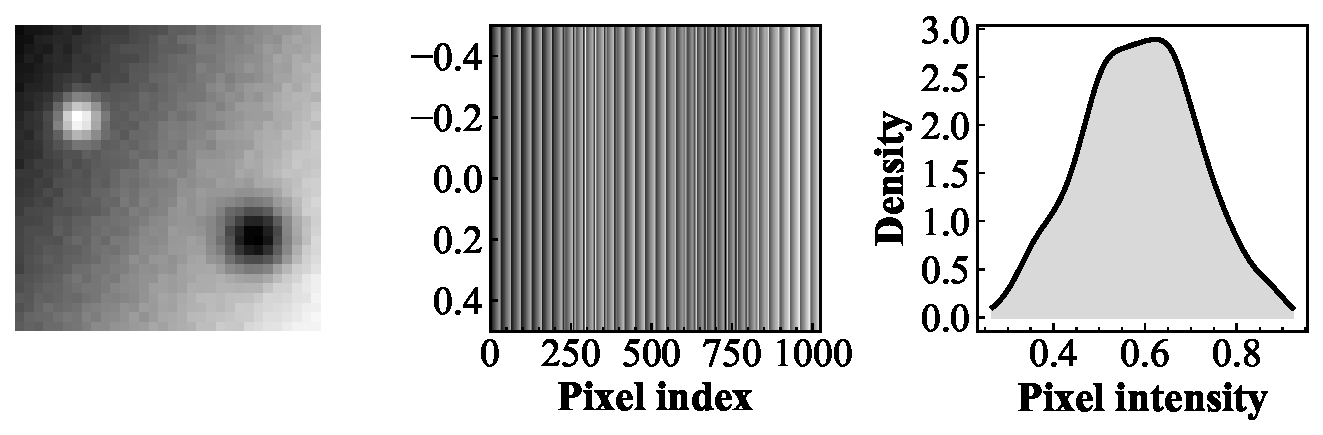
\includegraphics[width=.8\linewidth]{Figs/kde_image_density}
	\caption{Minh họa quá trình chuyển đổi dữ liệu ảnh thành hàm mật độ dựa trên màu sắc.}
	\label{fig:kdeimagedensity}
\end{figure}


\subsubsection{b.\qquad Ước lượng dựa vào khối màu}

Một hướng tiếp cận khác là phân chia ảnh thành các khối nhỏ có kích thước $s \times s$ và không chồng lắp từ phải sang trái, và từ trên xuống dưới. Mỗi ma trận vuông $P_k$ được ánh xạ thành véc tơ
\[
z_k = \mathrm{vec}(P_k) \in \mathbb{R}^{s^2}.
\]
Trong từng khối, tập hợp $\{z_{k,p}\}$ được coi là mẫu cục bộ. Với mỗi khối, tiến hành ước lượng mật độ bằng công thức hạt nhân Gauss, băng thông vẫn được lựa chọn theo quy tắc Silverman.  
Các hàm mật độ cục bộ $\hat{f}_k(u)$ là kết quả sau khi ước lượng cho từng khối.

Cách tiếp cận này duy trì thông tin màu sắc cho từng khối hình ảnh, phù hợp cho bài toán phân tích chùm vì sự phân biệt của nó trong các vùng màu sắc khác nhau. Hình~\ref{fig:kdepatchesdensity} thể hiện các khối màu được cắt từ hình ảnh gốc tại những vị trí lần lượt. Khối đầu chứa vùng sáng, khối cuối chứa vùng tối, hai khối còn lại nằm trên các vùng trung gian có mức xám thay đổi dần. Hàm mật độ của khối đầu có phân bố tập trung ở cường độ cao, thể hiện sự hiện diện của vùng sáng. Ngược lại, khối cuối có phân bố nghiêng về cường độ thấp phản ánh sự tồn tại của một vùng tối.

\begin{figure}[H]
	\centering
	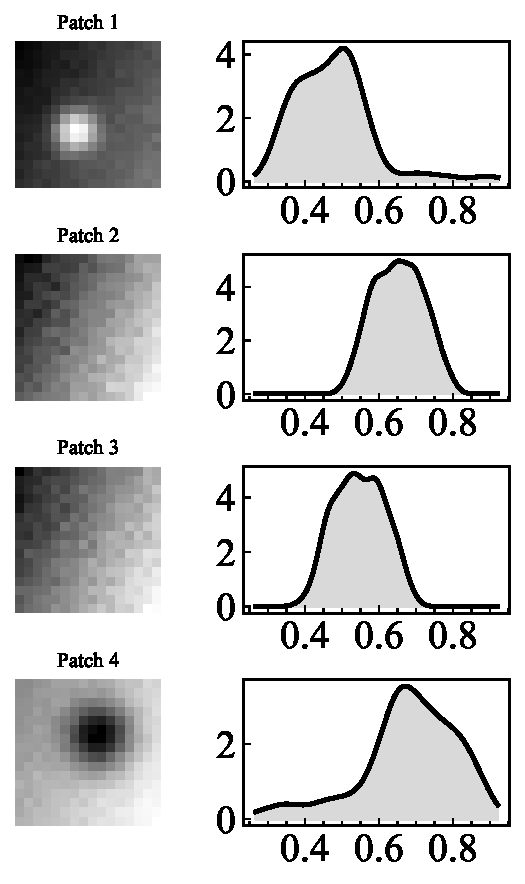
\includegraphics[width=0.55\linewidth]{Figs/kde_patches_density}
	\caption{Minh họa quá trình chuyển đổi dữ liệu ảnh thành hàm mật độ dựa trên khối màu.}
	\label{fig:kdepatchesdensity}
\end{figure}


\subsubsection{c.\qquad Ước lượng dựa vào vị trí điểm ảnh}

Thay vì chỉ xét giá trị cường độ, một cách tiếp cận khác là xem vị trí của các điểm ảnh như biến ngẫu nhiên. Cụ thể, với một hình ảnh $I \in \mathbb{R}^{M\times N}$, mỗi điểm ảnh $(i,j)$ được xem là một phần tử trong lưới tọa độ $\{1,\dots,M\}\times \{1,\dots,N\}$. Để xây dựng phân bố xác suất, ta chuẩn hóa cường độ của từng điểm ảnh theo công thức
\[
p_{ij} = \frac{I_{ij}}{\sum_{a=1}^M \sum_{b=1}^N I_{ab}}.
\]

Khi đó, ma trận $P = (p_{ij}) \in \mathbb{R}^{M\times N}$ được diễn giải như một phân phối xác suất rời rạc trên mặt phẳng tọa độ, phản ánh khả năng xuất hiện của một điểm ảnh tại vị trí $(i,j)$. Cách tiếp cận vị trí duy trì thông tin hình học của cấu trúc ảnh. Tùy vào bài toán và tính hợp lý của nó mà ta sử dụng các loại ước lượng khác nhau.

\begin{figure}[H]
	\centering
	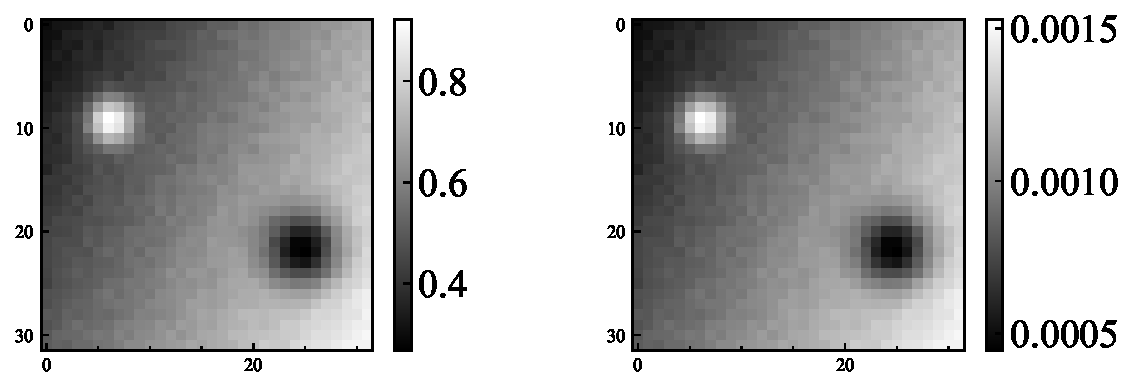
\includegraphics[width=.7\linewidth]{Figs/kde_position}
	\caption{Minh họa quá trình chuyển đổi dữ liệu ảnh thành hàm mật độ dựa trên vị trí.}
	\label{fig:kdeposition}
\end{figure}







\section{Ứng dụng của bài toán phân tích chùm}









\subsection{Dữ liệu}



\vdu{\label{vdu:anh1}
	Luận văn mô phỏng một tập dữ liệu ảnh mất cân bằng và định nghĩa trước hai chùm là sự khác biệt màu sắc của hai ảnh kết cấu. Hai ảnh gốc (kích thước $200\times 200$ pixel với $256$ mức xám) có cường độ nền khác nhau, $D83$ và $D102$. Những ảnh này được lấy từ cơ sở dữ liệu Kết cấu Brodatz tại \url{https://multibandtexture.recherche.usherbrooke.ca/original_brodatz.html} và được cắt ngẫu nhiên và phân bổ đều thành $64 \times 64$ ảnh. Sau đó, các ảnh được ghép lại thành một tập dữ liệu mất cân bằng với $IR$ dao động từ $10$ đến $70$.
	
	Hình~\ref{fig:EX2_main_img} minh họa một ảnh đã cắt và các hàm mật độ được trích xuất của nó. Khi xem xét Hình~\ref{fig:EX2_main}, chúng tôi nhận thấy thiếu sự khác biệt rõ ràng và nguy cơ mất cân bằng đáng kể trong tập dữ liệu. Chúng tôi nhận thức và chia nội dung của tập dữ liệu ảnh thành hai chùm do tính chất tiên nghiệm của nó ($D83$ và $D102$). Thách thức hiện tại là phân tích hình ảnh thành các chùm tương ứng một cách nhanh chóng.
	
	\begin{figure}[H]
		\centering
		\begin{subfigure}[b]{.4\linewidth}
			\centering
			
\includegraphics[width=.8\textwidth]{D82.png}
			\caption{$D83$}
		\end{subfigure}
		\begin{subfigure}[b]{.4\linewidth}
			\centering
			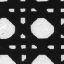
\includegraphics[width=.8\textwidth]{D102.png}
			\caption{$D102$}
		\end{subfigure}
		\caption{Các hình ảnh được cắt từ tập dữ liệu Brodatz.}\label{fig:EX2_main_img}
	\end{figure}
	
}


\vdu{\label{vdu:anh2}
Hình ảnh Landsat-8 ($512 \times 256$ pixel) bao phủ Đảo Yam cho thấy nguồn mất cân bằng ở cấp độ biển và đảo từ \url{https://oceancolor.gsfc.nasa.gov/}. Các bãi san hô nông, bãi cát nhỏ và các mảng thảm thực vật trên đảo bị áp đảo rất nhiều bởi các pixel ở vùng nước sâu. Độ lệch nghiêm trọng này đòi hỏi một thuật toán phân chùm mất cân bằng. Để phân đoạn ảnh này theo màu, trước tiên chúng tôi chuyển đổi ảnh thang độ xám và quét cửa sổ trượt các mảng $(p\times p)$ không chồng lấn từ trái sang phải, từ trên xuống dưới. Mỗi mảng giờ được làm phẳng thành một vectơ $(p\times p)$-pixel, hàm mật độ cường độ của nó được ước tính thông qua \texttt{ksdensity()}, và khối lập phương $(\text{patch}\times h\times\text{pdf})$ kết quả trên $3$-D được lưu trữ để phân chùm các mảng. Chiến lược này giữ lại các dấu hiệu đồng nhất địa phương và ngăn chặn việc ranh giới màu bị mờ. Ở đây, chúng tôi đặt kích thước khối màu bằng $4\times 4$.


\begin{figure}[H]
	\centering
	\begin{subfigure}[h]{0.40\textwidth}
		\centering
		
\includegraphics[width=\linewidth]{Fig/Yam_Island.png}
		\caption{Landsat Image}
	\end{subfigure}\hfill\\
	\begin{subfigure}[h]{0.47\textwidth}
		\centering
		
\includegraphics[width=\linewidth]{Fig/APP_pdf}
		\caption{Density of each pacthes ($4\times4$)}
	\end{subfigure}\hfill\\
	\caption{The real application image and its patches density function}
\end{figure}

}







\subsection{Phương pháp thực hiện}


\subsubsection{a.\qquad Ví dụ~\ref{vdu:anh1}}

Đối với Ví dụ



\subsubsection{b.\qquad Ví  dụ~\ref{vdu:anh2}}





\subsection{Kết quả thực hiện}


\subsubsection{a.\qquad Ví dụ~\ref{vdu:anh1}}

\subsubsection{b.\qquad Ví dụ~\ref{vdu:anh2}}





\section{Ứng dụng của bài toán phân loại}
\subsection{Dữ liệu}
\subsection{Phương pháp thực hiện}
\subsection{Kết quả thực hiện}


\newpage
\section{Bàn luận}




\subsection{Về phương pháp trích xuất hình ảnh}

Qua các ứng dụng ta có thể thấy, việc phân đoạn hay phân loại dữ liệu hình ảnh có thể dựa trên màu sắc đặc trưng của các đối tượng. Nó có thể đem lại kết quả chính xác mà không quá phức tạp. 

Tuy nhiên, việc trích xuất này cần một số tiền giả định về việc màu sắc phải cố định và hạn chế sai lệch. Vì sử dụng các thang màu RGB hoặc xám làm cho bài toán phân loại phải là phân loại màu sắc mà không phải hình dạng hay kết cấu. Ví dụ, việc trích xuất các loại củ quả như ớt chuông, củ cải, táo, các loại này có nhiều màu sắc (như táo đỏ, táo xanh) nên không thể dùng trích xuất loại này. Hơn nữa, các sai lệch về độ sáng của hình ảnh cũng ảnh hưởng đến kết quả trích xuất.

\subsection{Về thuật toán phân tích chùm các hàm mật độ xác suất}


Phân tích chùm phân vùng dựa vào trọng tâm rất đơn giản. 


Tuy nhiên, nó cũng có một số khuyết điểm bao gồm tính không xác định của các siêu tham số\index{siêu tham số (hyper-parametre)},  chất lượng dữ liệu đầu vào và khả năng giải thích của mô hình. Đầu tiên, họ thuật toán này không cung cấp $c$ chùm tối ưu. Đôi khi, ta không có tri thức về số lượng $c$, dẫn đến khó khăn khi phân chùm các mẫu có số chiều lớn \cite{schubert2023stop}, và nguy cơ quá khớp\index{quá khớp (overfitting)}. Theo Goutte \textit{et al.}, ``\emph{khi số lượng chùm không phản ánh trong dữ liệu, kết quả cuối cùng cơ bản là vô nghĩa}'' \cite{goutte1999clustering}.  Ngoài ra, do giả định tối ưu lồi, thuật toán dựa trên trọng tâm thường hoạt động hiệu quả nhất với hình dạng gần cầu, và có thể gặp thách thức khi áp dụng cho dữ liệu chứa nhiễu, ngoại lệ\index{điểm ngoại lệ (outliers)}, có chồng lấp giữa các chùm hoặc có sự chênh lệch lớn về kích thước và mật độ. Cuối cùng, hàm mật độ trọng tâm chùm ban đầu cũng ảnh hưởng đến kết quả tối ưu dù đã có nhiều khuyến nghị như $k$-means$^{++}$\index{$k$-means$^{++}$}. 
	
	Ngược lại, phân tích chùm thứ bậc không đòi hỏi tiên nghiệm về số chùm, nhưng chi phí tính toán cao, đặc biệt với dữ liệu lớn khi cần tính toàn bộ ma trận khoảng cách


Tóm lại, các thuật toán phân tích chùm mang lại tiềm năng lớn trong việc khám phá các cấu trúc ẩn và những mối quan hệ có ý nghĩa giữa các mẫu dữ liệu, từ đó hỗ trợ các phân tích chuyên sâu và mở ra nhiều ứng dụng tiềm năng \cite{nguyen2024new,nguyentrang2017fuzzy}. Mặc dù kết quả của các thuật toán phân tích chùm có thể chịu ảnh hưởng bởi dữ liệu đầu vào, thể loại tự nhiên và lựa chọn thuật toán, chúng vẫn đóng vai trò là công cụ mạnh mẽ giúp người dùng nhận diện và diễn giải các mẫu tốt hơn. Qua đó, \emph{các loại tự nhiên có là những gì thuật toán phân chùm phần nào hướng đến trong điều kiện lý tưởng không} là một chủ đề nghiên cứu đầy hứa hẹn, tiếp tục được quan tâm và mở rộng trong cộng đồng khoa học thống kê \cite{leonelli2019data,watson2023philosophy,watson2023reply,mollema2024responding}.



\subsection{Về thuật toán phân tích chùm các hàm mật độ xác suất}

\subsection{Về thuật toán phân loại các hàm mật độ xác suất}
















\section*{Tổng kết chương \ref{chapter_3}}
\addcontentsline{toc}{section}{Tổng kết chương \ref{chapter_3}}

\chapter*{PHẦN KẾT LUẬN}\label{chapter_ketluan}
\addcontentsline{toc}{chapter}{PHẦN KẾT LUẬN}

\section*{1\quad Kết luận}

Nhận dạng thống kê cho hàm mật độ xác suất là một chủ đề mới vì cho đến hiện tại các lý thuyết và ứng dụng của nó đều cần nhiều nỗ lực xây dựng.

\section*{2\quad Định hướng nghiên cứu}




%\chapter*{THỜI GIAN LÀM LUẬN VĂN}\label{time}
%\addcontentsline{toc}{chapter}{THỜI GIAN LÀM LUẬN VĂN}


%\begin{enumerate}
%	\item Thu thập tài liệu 05/2024 -- 09/2024
%	\item Viết và báo cáo đề cương: 09/2024 -- 10/2024
%	\item Viết chương 1: 10/2024 --12/2024
%	\item Viết chương 2: 12/2025 -- 03/2025
%	\item Viết chương 3: 03/2025 -- 06/2025
%	\item Hoàn chỉnh luận văn: 06/2025 -- 07/2025
%	\item Chuẩn bị và thực hiện báo cáo luận văn: 07/2025 -- 08/2025
%\end{enumerate}



%%%%%%%%%%%% Tài liệu tham khảo %%%%%%%%%%%%
\addcontentsline{toc}{chapter}{\numberline{TÀI LIỆU THAM KHẢO}}%
\bibliographystyle{ieeetr}
%\bibliographystyle{apacite}

{\fontsize{11}{15pt}\selectfont
\bibliography{Tailieu}
}




%\clearpage
%\pagenumbering{roman}	
%\appendix

\chapter*{PHỤ LỤC A\\MÃ NGUỒN}
\addcontentsline{toc}{chapter}{PHỤ LỤC}

Về tài nguyên tính toán, luận văn này chạy trên hệ điều hành Ubuntu 24.04.2 LTS, nhân Linux 6.11.0-19-generic, 11th Gen Intel$\copyright$ Core$^\text{TM}$ i5-11400H$\times$12, bộ nhớ 16.0 GiB. 

Việc thực thi mã nguồn được sử dụng trong môi trường ảo\index{môi trường ảo (virtual environment)} của Anaconda tên là `\texttt{proclustEnv}'. Các mã Python được sử dụng trong luận văn này được lưu trữ tại \url{https://github.com/hungtrannam/probclust}. Các thư viện trên được lưu trong tệp \texttt{requirements.yml} và có thể được cài đặt tự động bằng lệnh 
{\small
	\begin{verbatim}
conda install environment.yml
	\end{verbatim}
}
Đây là danh sách các thư viện Python cần thiết để thực thi toàn bộ mã nguồn trong luận văn. 

{\small

\begin{verbatim}

\end{verbatim}
}






\chapter*{PHỤ LỤC B\\KẾT QUẢ}\label{phulucB}



\vdu{[Liên kết các chùm hàm mật độ]\label{VD:dist} 
Giả sử ta có ba chùm hàm mật độ xác suất Gauss $\mathcal{F}\,;\mathcal{G}$ và $\mathcal{H}$. Tính các liên kết $\Delta(\mathcal{F}\,;\mathcal{G})$ và $\Delta(\mathcal{F}\cup\mathcal{G}\,;\mathcal{H})$ biết khoảng cách giữa hai hàm mật độ là $\mathcal{L}_2$ và các chùm
\begin{align*}
\mathcal{F} &= \{f_1=\mathcal{N}(0,3\,;1),\, f_2=\mathcal{N}(1\,;1)\}, \\
\mathcal{G} &= \{g_1=\mathcal{N}(4,0\,;1),\, g_2=\mathcal{N}(5,5\,;1),\, g_3=\mathcal{N}(4,8\,;1)\},\\
\mathcal{H} &= \{h_1=\mathcal{N}(9,1\,;1),\, h_2=\mathcal{N}(8,0\,;1)\}.\\
\end{align*}

}

	
	\paragraph{Bài giải  \ref{VD:dist}.} Vì các phương sai của hàm mật độ Gauss đều bằng 1. Nên ta có thể tính $\mathcal{L}_2$ bằng công thức tổng quát 
	$
	\mathcal{L}_2(u\,;v)=\left(2-2\exp\left(-\frac{(\mu_u-\mu_v)^2}{4\sigma^2}\right)\right)^{1/2}.
	$
	Sau khi tính toán, ta nhận được ma trận khoảng cách từng đôi một.
	$$
	\begin{array}{c|ccccccc}
		& \left\{f_1\right.     & \left.f_2\right\}     & \left\{g_1\right.     & g_2     & \left.g_3\right\}     & \left\{h_1\right.     & \left.h_2\right\}     \\
		\hline
		f_1     &         &         &         &         &         &         &         \\
		f_2     & 0{,}26  &         &         &         &         &         &         \\
		g_1     & 0{,}74  & 0{,}71  &         &         &         &         &         \\
		g_2     & 0{,}75  & 0{,}75  & 0{,}49  &         &         &         &         \\
		g_3     & 0{,}75  & 0{,}74  & 0{,}29  & 0{,}26  &         &         &         \\
		h_1     & 0{,}75  & 0{,}75  & 0{,}75  & 0{,}74  & 0{,}75  &         &         \\
		h_2     & 0{,}75  & 0{,}75  & 0{,}74  & 0{,}67  & 0{,}72  & 0{,}38  &         
	\end{array}
	$$
	Từ đây, ta có thể dễ dàng tính được các liên kết $\Delta(\mathcal{F},\, \mathcal{G}) $ thông qua ma trận này. Ta có,
	\begin{align*}
		\Delta_{\min}(\mathcal{F},\, \mathcal{G}) &= \min\big\{
		\mathcal{L}_2(f_1, g_1),\, \mathcal{L}_2(f_1, g_2),\, \mathcal{L}_2(f_1, g_3),\,
		\mathcal{L}_2(f_2, g_1),\, \mathcal{L}_2(f_2, g_2),\, \mathcal{L}_2(f_2, g_3)
		\big\} \\
		&=\min\{0{,}74;\ 0{,}75;\ 0{,}75;\ 0{,}71;\ 0{,}75;\ 0{,}74\} = {0{,}71},\\
		\Delta_{\max}(\mathcal{F},\, \mathcal{G}) &= \max\big\{
		\mathcal{L}_2(f_1, g_1),\, \mathcal{L}_2(f_1, g_2),\, \mathcal{L}_2(f_1, g_3),\,
		\mathcal{L}_2(f_2, g_1),\, \mathcal{L}_2(f_2, g_2),\, \mathcal{L}_2(f_2, g_3)
		\big\}\\
		&	= \max\{0{,}74;\, 0{,}75;\, 0{,}75;\, 0{,}71;\, 0{,}75;\, 0{,}74\} = {0{,}75},\\
		\Delta_{\text{avg}}(\mathcal{F},\, \mathcal{G}) &= \frac{1}{6} \sum_{\substack{f \in \mathcal{F} \\ g \in \mathcal{G}}} \mathcal{L}_2(f, g) = 
		0{,}17(0{,}74 + 0{,}75 + 0{,}75 + 0{,}71 + 0{,}75 + 0{,}74) =  {0{,}74},\\
		\Delta_{\text{centroid}}(\mathcal{F}, \mathcal{G}) &=\mathcal{L}_2(\theta_\mathcal{F}\,;\theta_{\mathcal{G}})= \left(2 - 2 \exp\left(-\frac{(0{,}65 - 4{,}77)^2}{4}\right)\right)^{1/2}
		= {1{,}41},\\ &\text{ với } \theta_{\mathcal{F}} = (0{,}3 + 1{,}0)/2 = 0{,}65\,; \theta_{\mathcal{G}} =(4{,}0 + 5{,}5 + 4{,}8)/3 = 4{,}77,\\
		\Delta_{\text{Ward}}(\mathcal{F}, \mathcal{G}) &= \frac{\#\mathcal{F} \cdot \#\mathcal{G}}{\#\mathcal{F} + \#\mathcal{G}} \cdot \mathcal{L}_2^2(\theta_{\mathcal{F}}, \theta_{\mathcal{G}})
		= \frac{2 \cdot 3}{2 + 3} \cdot \left(1{,}41\right)^2 = {2{,}39},
	\end{align*}
	
	
	Tương tự, ta cũng có kết quả cho $\Delta(\mathcal{F}\cup\mathcal{G}\,;\mathcal{H})$ là
	\begin{align*}
		\Delta_{\min}(\mathcal{F} \cup \mathcal{G},\, \mathcal{H}) &= {0{,}67}\,; \Delta_{\max}(\mathcal{F} \cup \mathcal{G},\, \mathcal{H}) = {0{,}75}\,;
		\Delta_{\text{avg}}(\mathcal{F} \cup \mathcal{G},\, \mathcal{H}) = {0{,}74},\\
		\Delta_{\text{centroid}}(\mathcal{F} \cup \mathcal{G},\, \mathcal{H}) &= {1{,}41}\,; \Delta_{\text{Ward}}(\mathcal{F} \cup \mathcal{G},\, \mathcal{H}) = {2{,}86}.\\
	\end{align*}


\paragraph{Bài giải Ví dụ~\ref{VD:thubac}.} Đầu tiên, ta xem thứ tự của $\mu_i$ chính là thứ tự của dữ liệu hàm mật độ $f_i$, tính toán các khoảng cách từng đôi hàm mật độ bất kỳ bằng khoảng cách $\mathcal{L}_2(f_i\,;f_j)$ với $i\,;j = 1\,;\ldots\,;7$, ta nhận được ma trận khoảng cách
$$
\bm D^{(t=0)} =
\begin{array}{c|ccccccc}
	& f_1     & f_2     & f_3     & f_4     & f_5     & f_6     & f_7     \\
	\hline
	f_1 &        &        &        &        &        &        &        \\
	f_2 & 0{,}74 &        &        &        &        &        &        \\
	f_3 & 0{,}75 & 0{,}75 &        &        &        &        &        \\
	f_4 & \mathbf{0{,}26} & 0{,}71 & 0{,}75 &        &        &        &        \\
	f_5 & 0{,}75 & 0{,}49 & 0{,}74 & 0{,}75 &        &        &        \\
	f_6 & 0{,}75 & 0{,}74 & 0{,}38 & 0{,}75 & 0{,}67 &        &        \\
	f_7 & 0{,}75 & 0{,}29 & 0{,}75 & 0{,}74 & \mathbf{0{,}26} & 0{,}72 &       
\end{array}
$$

Ta thấy khoảng cách $D(f_1\,;f_4) = D(f_5\,;f_7)  = 0,26$ là khoảng cách nhỏ nhất nên ta chọn một trong hai. Trường hợp này, ta chọn hàm mật độ $f_1$ và $f_4$ xếp vào một chùm $\{f_1\,;f_4\}$. Tiến hành tính toán liên kết đủ giữa chùm $\{f_1\,;f_4\}$ với các hàm mật độ khác. Ta có
\begin{align*}
	\Delta(\{f_1\,;f_4\}\,; f_2)=\max\{D(f_1\,;f_2)\,; D(f_4\,;f_2)\} = \max\{0,74\,;0,71\} = 0,74,\\
	\Delta(\{f_1\,;f_4\}\,; f_3)=\max\{D(f_1\,;f_3)\,; D(f_4\,;f_3)\} = \max\{0,75\,;0,75\} = 0,75,\\
	\Delta(\{f_1\,;f_4\}\,; f_5)=\max\{D(f_1\,;f_5)\,; D(f_4\,;f_5)\} = \max\{0,75\,;0,75\} = 0,75,\\
	\Delta(\{f_1\,;f_4\}\,; f_6)=\max\{D(f_1\,;f_6)\,; D(f_4\,;f_6)\} = \max\{0,75\,;0,75\} = 0,75,\\
	\Delta(\{f_1\,;f_4\}\,; f_7)=\max\{D(f_1\,;f_7)\,; D(f_4\,;f_7)\} = \max\{0,75\,;0,74\} = 0,75.\\
\end{align*}

Ta xóa dòng/cột $f_1$ và $f_4$ và thay bằng một dòng/cột mới là $\{f_1\,;f_4\}$, ta được ma trận khoảng cách mới
\[
\bm D^{(t=1)} =
\begin{array}{c|cccccc}
	& \{f_1\,;f_4\} & f_2   & f_3   & f_5   & f_6   & f_7 \\
	\hline
	\{f_1\,;f_4\}  &        &        &        &        &        &        \\
	f_2     & 0{,}74 &        &        &        &        &        \\
	f_3     & 0{,}75 & 0{,}75 &        &        &        &        \\
	f_5     & 0{,}75 & 0{,}49 & 0{,}74 &        &        &        \\
	f_6     & 0{,}75 & 0{,}74 & 0{,}38 & 0{,}67 &        &        \\
	f_7     & 0{,}75 & 0{,}29 & 0{,}75 & \mathbf{0{,}26} & 0{,}72 &        
\end{array}
\]


Tiếp theo, ta thấy $D(f_5\,;f_7) = 0,26$ là cách nhỏ nhất nên ta xếp hai hàm mật độ này thành một chùm mới $\{f_5\,;f_7\}$. Tiến hành tính toán liên kết đủ giữa chùm $\{f_5\,;f_7\}$ với các hàm mật độ khác. Ta có
\begin{align*}
	\Delta(\{f_5\,;f_7\}\,; \{f_1\,;f_4\})&=\max\{D(f_5\,;f_1)\,; D(f_5\,;f_4)\,; D(f_7\,;f_1)\,; D(f_7\,;f_4)\} =0,75,\\
	\Delta(\{f_5\,;f_7\}\,; f_2)&=\max\{D(f_5\,;f_2)\,; D(f_7\,;f_2)\} = 0,49,\\
	\Delta(\{f_5\,;f_7\}\,; f_3)&=\max\{D(f_5\,;f_3)\,; D(f_7\,;f_3)\} = 0,75,\\
	\Delta(\{f_5\,;f_7\}\,; f_6)&=\max\{D(f_5\,;f_6)\,; D(f_7\,;f_6)\} = 0,72.\\
\end{align*}

Ta xóa dòng/cột $f_5$ và $f_7$ và thay bằng một dòng/cột mới là $\{f_5\,;f_7\}$, ta được ma trận khoảng cách mới
\[
\bm D^{(t=2)} =
\begin{array}{c|ccccc}
	& \{f_1,f_4\} & f_2   & f_3   & \{f_5,f_7\} & f_6\\
	\hline
	\{f_1,f_4\}   &         &        &        &      &  \\
	f_2           & 0{,}75  &        &        &   &    \\
	f_3           & 0{,}75  & 0{,}75 &        &    &    \\
	\{f_5,f_7\}   & 0{,}75  & {0{,}49} & 0{,}75 &     \\
	f_6 &0,75&0,74&\textbf{0,38}& 0,72\\   
\end{array}
\]

Tiếp theo, ta thấy $D(f_3\,;f_6) = 0,38$ là cách nhỏ nhất nên ta xếp hai hàm mật độ này thành một chùm mới $\{f_3\,;f_6\}$. Tiến hành tính toán liên kết đủ giữa chùm $\{f_3\,;f_6\}$ với các hàm mật độ khác. Ta có
\begin{align*}
	\Delta(\{f_3\,;f_6\}\,; \{f_1\,;f_4\})&=\max\{D(f_3\,;f_1)\,; D(f_3\,;f_4)\,; D(f_6\,;f_1)\,; D(f_6\,;f_4)\} =0,75,\\
	\Delta(\{f_3\,;f_6\}\,; \{f_5\,;f_7\})&=\max\{D(f_3\,;f_5)\,; D(f_3\,;f_7)\,; D(f_6\,;f_5)\,; D(f_6\,;f_7)\} =0,75,\\
	\Delta(\{f_3\,;f_6\}\,; f_2)&=\max\{D(f_5\,;f_3)\,; D(f_7\,;f_3)\} = 0,75,\\
\end{align*}

Ta xóa dòng/cột $f_3$ và $f_6$ và thay bằng một dòng/cột mới là $\{f_3\,;f_6\}$, ta được ma trận khoảng cách mới
\[
\bm D^{(t=3)} =
\begin{array}{c|cccc}
	& \{f_1,f_4\} & f_2   & \{f_5,f_7\} & \{f_3,f_6\} \\
	\hline
	\{f_1,f_4\}     &         &        &        &        \\
	f_2             & 0{,}75  &        &        &        \\
	\{f_5,f_7\}     & 0{,}75  & \textbf{0{,}49} &       &        \\
	\{f_3,f_6\}     & 0{,}75  & 0{,}75 & 0{,}75 &        
\end{array}
\]

Tiếp theo, ta thấy $D(\{f_5\,;f_7\}\,;f_2) = 0,49$ là cách nhỏ nhất nên ta xếp hàm mật độ $f_2$ này vào chùm $\{f_5\,;f_7\}$. Tiến hành tính toán liên kết đủ giữa chùm $\{f_2\,;f_5\,;f_7\}$ với các hàm mật độ khác. Ta có
\begin{align*}
	\Delta(\{f_2, f_5, f_7\}, \{f_1, f_4\}) &= \max\{ D(f_2\,; \{f_1\,;f_4\}), D(f_5\,; \{f_1\,;f_4\}), D(f_7\,; \{f_1\,;f_4\}) \} = 0{,}75, \\
	\Delta(\{f_2, f_5, f_7\}, \{f_3, f_6\}) &= \max\{ D(f_2\,; \{f_3\,;f_6\}), D(f_5\,; \{f_3\,;f_6\}), D(f_7\,; \{f_3\,;f_6\}) \} = 0{,}75.
\end{align*}

Ta xóa dòng/cột $f_2$ và $\{f_5\,;f_7\}$ và thay bằng một dòng/cột mới là $\{f_2\,;f_5\,;f_7\}$, ta được ma trận khoảng cách mới
\[
\bm D^{(t=4)} =
\begin{array}{c|ccc}
	& \{f_1,f_4\} & \{f_2,f_5,f_7\} & \{f_3,f_6\} \\
	\hline
	\{f_1,f_4\}        &         &        &        \\
	\{f_2,f_5,f_7\}    &0,75 &        &        \\
	\{f_3,f_6\}        & 0,75  & \textbf{0,75}&        
\end{array}
\]

Cuối cùng, ta chọn xếp chùm $\{f_2,f_5,f_7\}$  vào chùm $\{f_3,f_6\}$ dựa vào khoảng cách chính xác nhỏ nhất (4 chữ số thập phân). Vậy ta có chùm $\{f_2\,;f_5\,;f_3\,;f_6\}$. Ta xếp chùm còn lại vào chùm mới này, thuật toán kết thúc. 


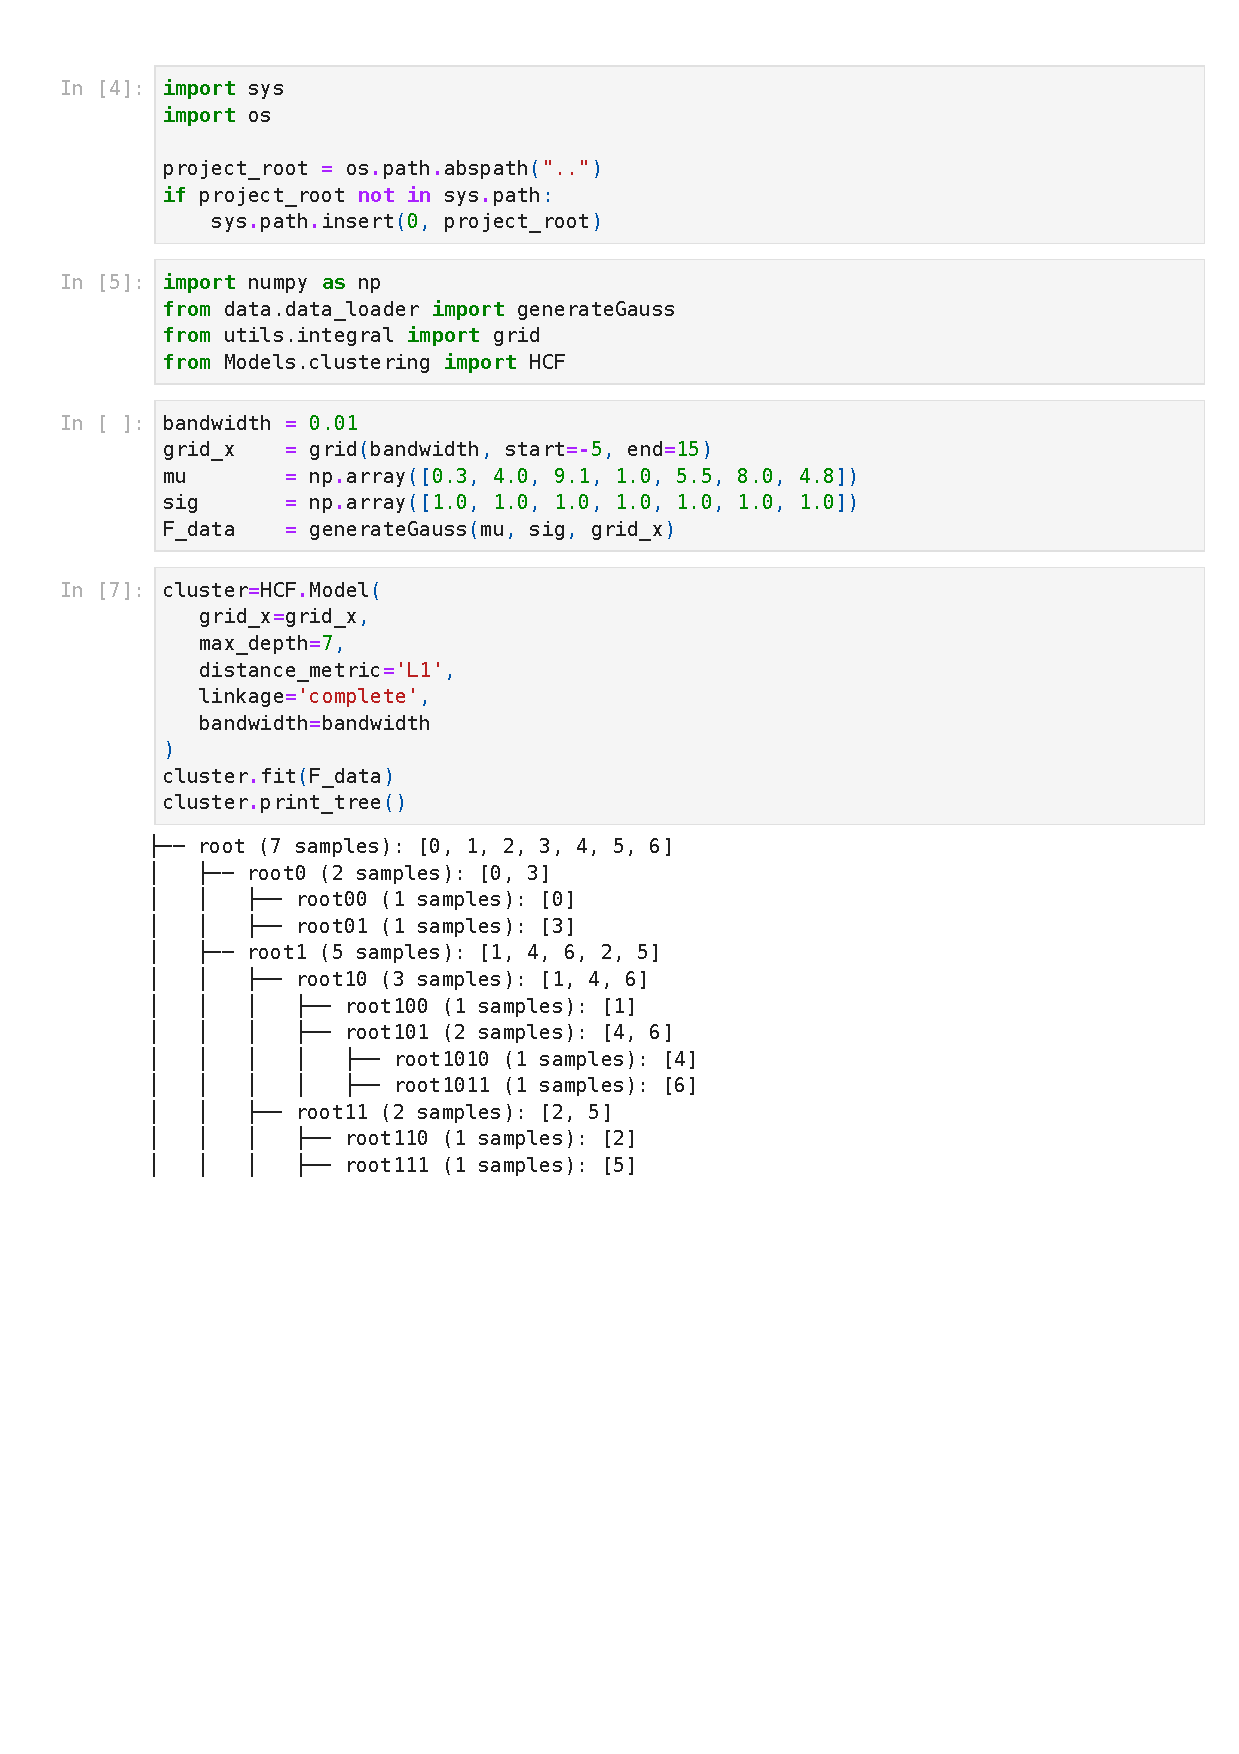
\includepdf[pages=-]{HCF.pdf}

\paragraph{Bài giải Ví dụ~\ref{VD:FCF}.}
Cho $c=3$, $\epsilon=10^{-3}$, Các trọng tâm khởi tạo ngẫu nhiên bởi
$\theta_1(x)\!\sim\!\mathcal N(0;1)$, 
$\theta_2(x)\!\sim\!\mathcal N(2;1)$, 
$\theta_3(x)\!\sim\!\mathcal N(5;1)$.
 Ta cũng khởi tạo các phần tử trong ma trận $\bm U$ tuân theo phân phối Dirichlet. 
Ma trận khoảng cách $\bm D$ trong đó hàng $i$ là $\theta_i$, cột $j$ là $f_j$, các khoảng cách được tính bởi $\mathcal{L}_2$ dựa vào trọng tâm và phân vùng như sau

\begin{figure}[H]
	\centering
	\begin{subfigure}{.48\textwidth}
			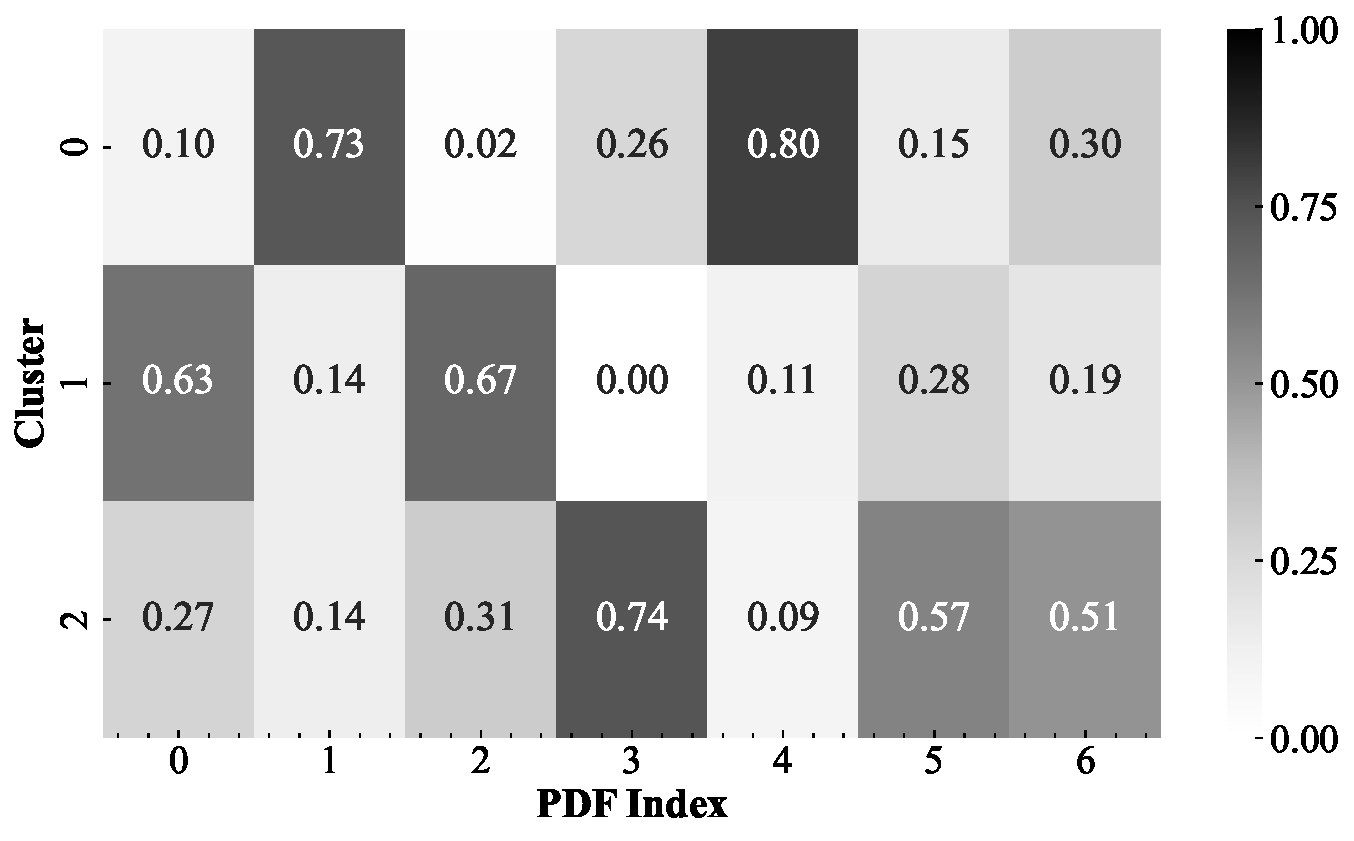
\includegraphics[width=\textwidth]{FCF_U0}
			\caption{Ma trận phân vùng $\bm U$}
	\end{subfigure}
	\begin{subfigure}{.48\textwidth}
	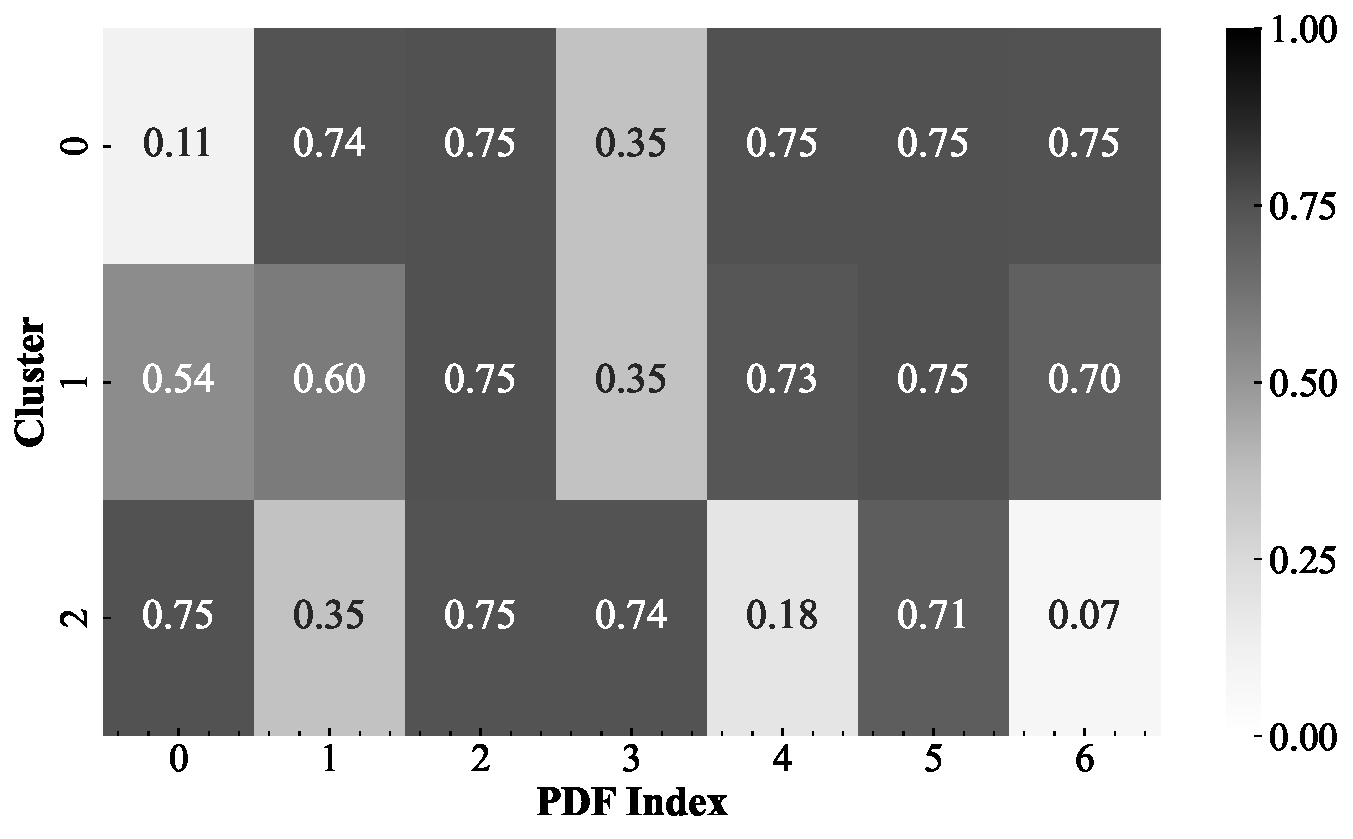
\includegraphics[width=\textwidth]{FCF_D0}
	\caption{Ma trận khoảng cách $\bm D$}
\end{subfigure}
\caption{Khởi tạo ngẫu nhiên của FCF}\label{fig:UD0}
\end{figure}

%======================== D(0): TỪỜNG MINH ========================
Khoảng cách $\bm D^{(t=0)}$ với $\mathcal{L}_2=\|\,\mathcal N(\mu;1)-\mathcal N(\nu;1)\,\|_2
=\left[\frac{1}{\sqrt\pi}\!\left(1-e^{-(\mu-\nu)^2/4}\right)\right]^{1/2}$, ta có
\[
\begin{aligned}
	D_{11}&=\Bigl[\tfrac{1}{\sqrt\pi}\!\bigl(1-e^{-(0{,}3)^2/4}\bigr)\Bigr]^{1/2}= 0{,}11,\\
	D_{21}&=\Bigl[\tfrac{1}{\sqrt\pi}\!\bigl(1-e^{-(1{,}7)^2/4}\bigr)\Bigr]^{1/2}= 0{,}54,\\
	D_{31}&=\Bigl[\tfrac{1}{\sqrt\pi}\!\bigl(1-e^{-(4{,}7)^2/4}\bigr)\Bigr]^{1/2}= 0{,}75.
\end{aligned}
\]
Tóm lại, ta thu được ma trận khoảng cách $\bm D$ tại Hình~\ref{fig:UD0}(b). Hơn nữa,
%======================== U(1): TỪỜNG MINH ========================
Ma trận phân vùng $\bm U^{(1)}$ với $m=2$ cũng được tính toán như sau. Vì không có $D_{ij}=0$ nên dùng công thức cập nhật từ \eqref{pvFCF1}, ta có
$
u_{ij}^{(1)}=\left(\sum_{k=1}^{3}\left(\frac{D_{ij}}{D_{kj}}\right)^{2}\right)^{-1}\,;\forall j.$ Suy ra ta thu được ma trận phân vùng $\bm U$ (tại Hình~\ref{fig:UD0}(a)) từ cách tính cho cột $j=1$ như sau
\[
\begin{aligned}
	u_{11}&=\left [1+\left (\frac{0{,}112}{0{,}54}\right )^{2}+\left (\frac{0{,}11}{0{,}75}\right )^{2}\right ]^{-1}= 0{,}94,\\
	u_{21}&=\left [\left (\frac{0{,}54}{0{,}11}\right )^{2}+1+\left (\frac{0{,}54}{0{,}75}\right )^{2}\right ]^{-1}= 0{,}04,\\
	u_{31}&=\left [\left(\frac{0{,}75}{0{,}11}\right )^{\!2}+\left (\frac{0{,}75}{0{,}54}\right )^{2}+\right ]^{-1}= 0{,}02.
\end{aligned}
\]


\begin{figure}[H]
	\centering
	\begin{subfigure}{.48\textwidth}
		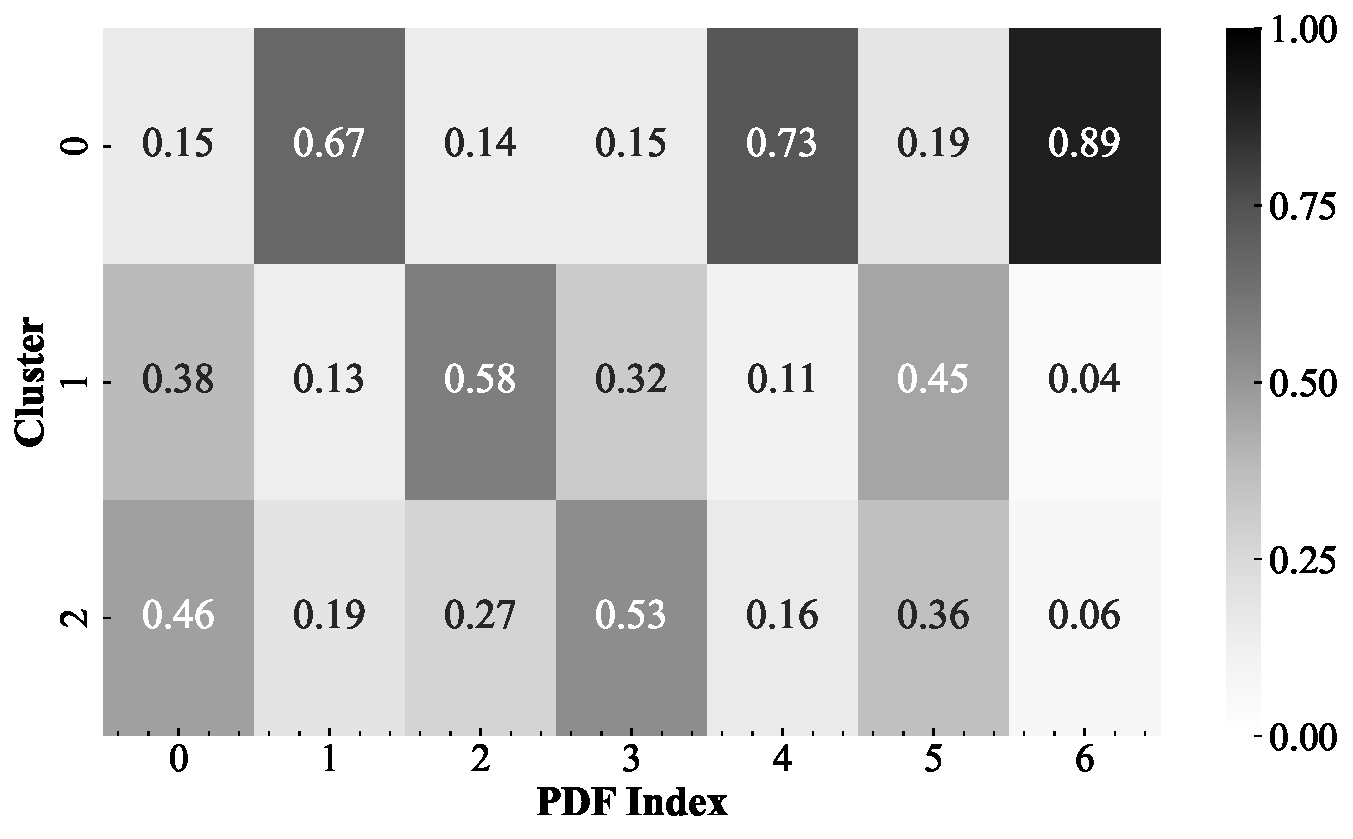
\includegraphics[width=\textwidth]{FCF_U1}
		\caption{Ma trận phân vùng $\bm U$}
	\end{subfigure}
	\begin{subfigure}{.48\textwidth}
		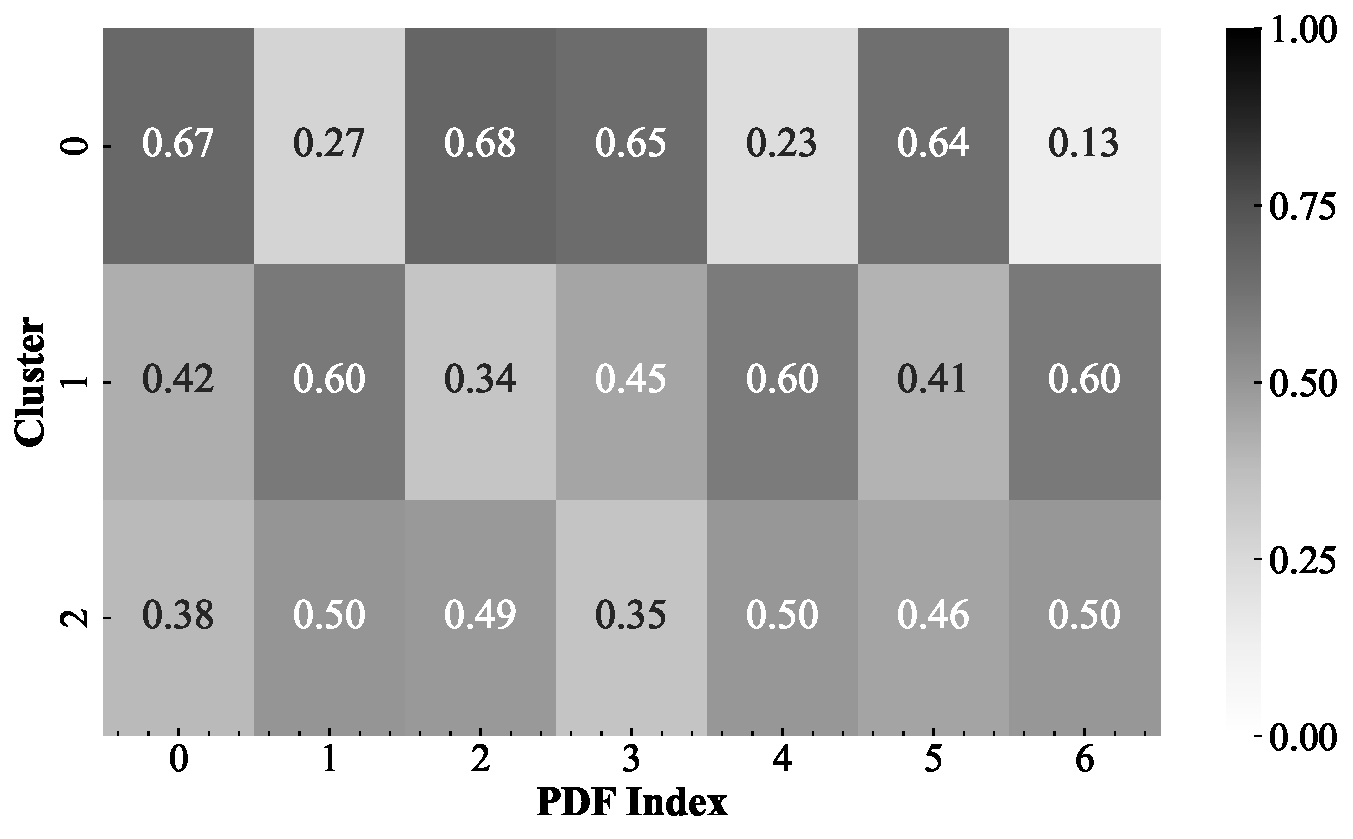
\includegraphics[width=\textwidth]{FCF_D1}
		\caption{Ma trận khoảng cách $\bm D$}
	\end{subfigure}
	\caption{Vòng lặp $t=1$ của FCF}
\end{figure}


Gom toàn bộ cột, ta nhận được ma trận phân vùng sau vòng lặp đầu tiên là $\bm U$. Với chuẩn \(\mathcal L_2\) trên hàm, theo \eqref{pvFCF2}. Để tính toán tiêu chuẩn dừng, ta tính theo công thức $$\left\Vert {\bm\mu}^{(t+1)} - {\bm\mu}^{(t)} \right \Vert = 0,96.$$ Vì chuẩn này chưa nhỏ hơn tiêu chuẩn dừng, ta tiếp tục lặp lại quá trình trên. Sau $t=9$ vòng lặp, thuật toán FCF dừng với chuẩn là $6,12\times 10^{-4}$.


\begin{figure}[H]
	\centering
	\begin{subfigure}{.48\textwidth}
		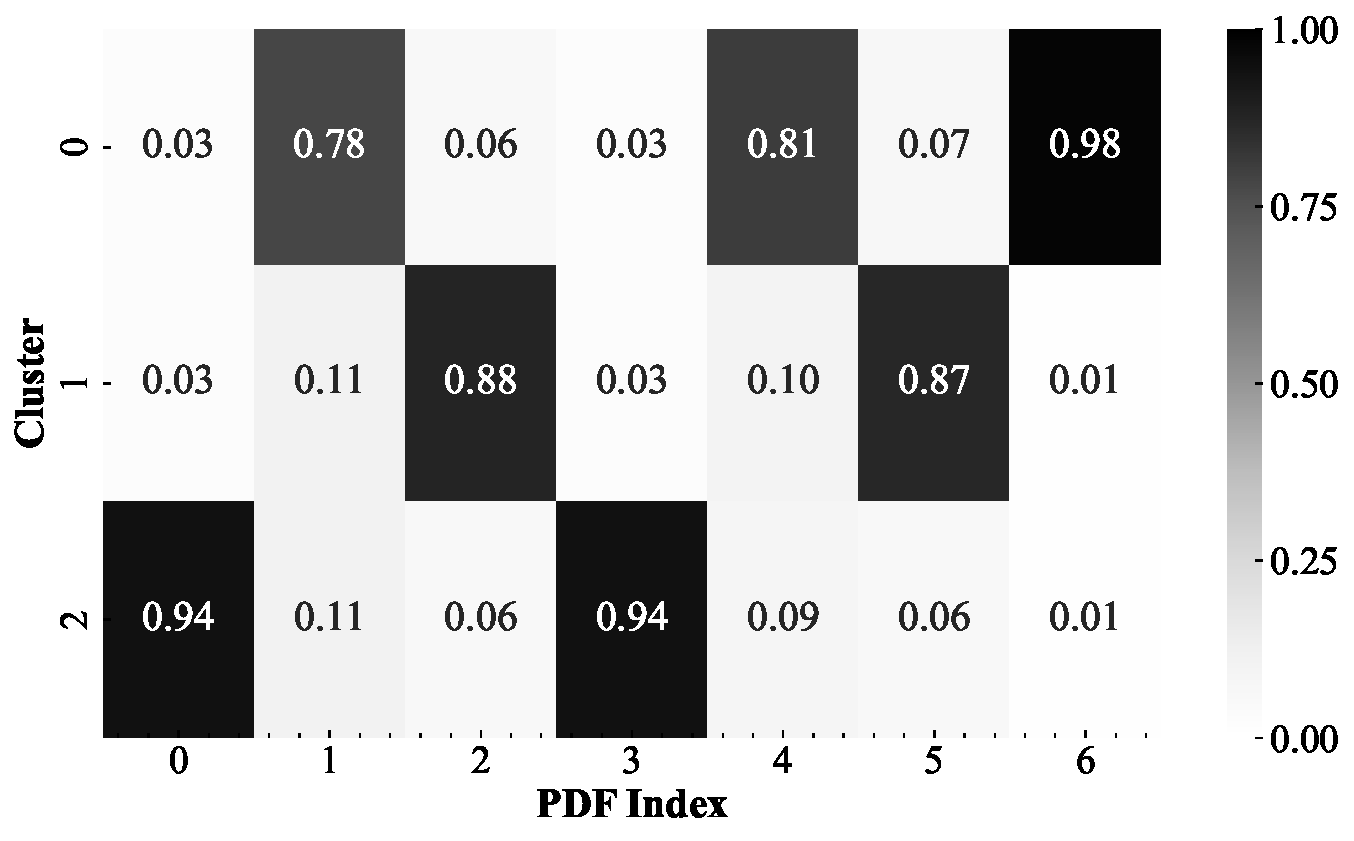
\includegraphics[width=\textwidth]{FCF_U9}
		\caption{Ma trận phân vùng $\bm U$}
	\end{subfigure}
	\begin{subfigure}{.48\textwidth}
		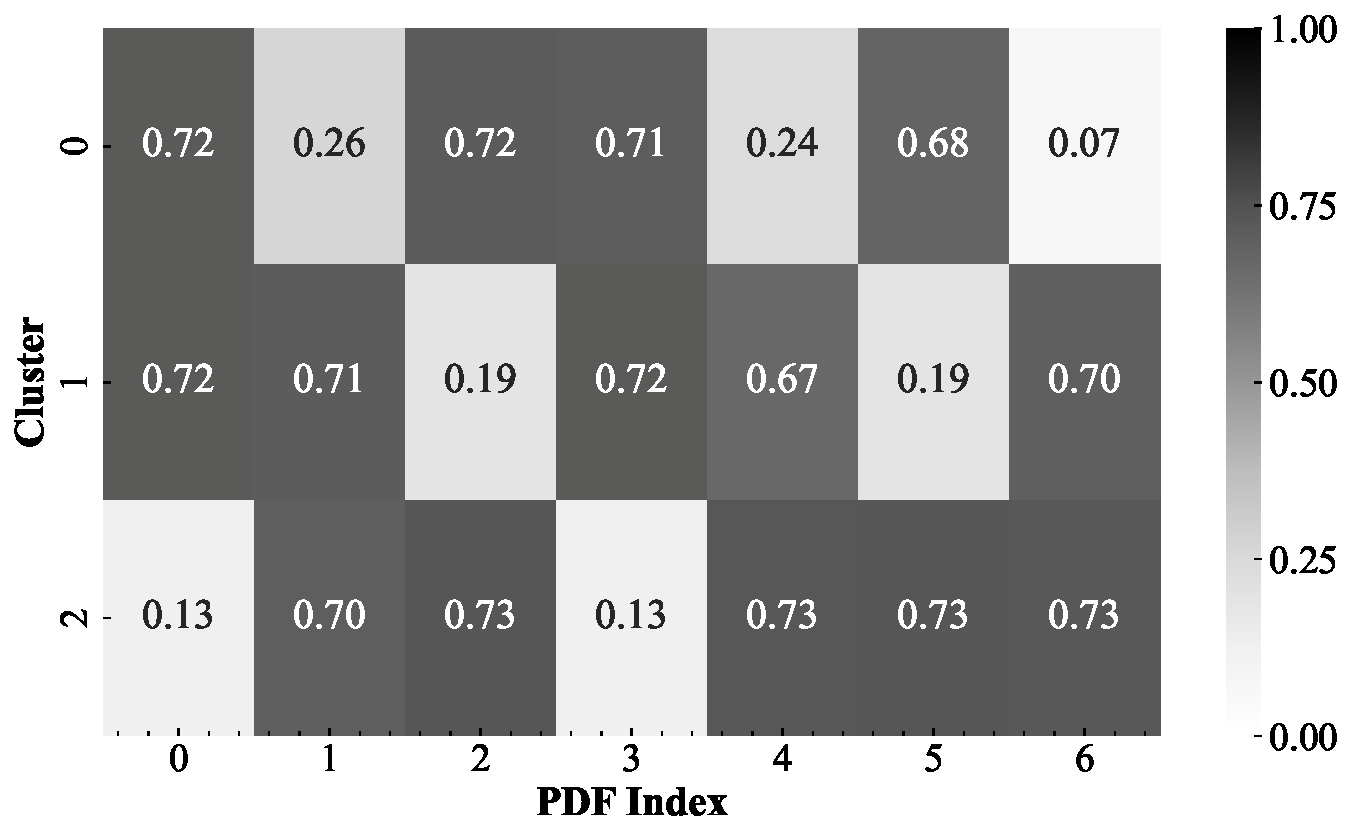
\includegraphics[width=\textwidth]{FCF_D9}
		\caption{Ma trận khoảng cách $\bm D$}
	\end{subfigure}
	\caption{Vòng lặp $t=9$ của FCF}
\end{figure}


Ta có quá trình biến đổi ở mỗi vòng lặp đối với các trọng tâm ở Hình~\ref{fig:vdu:trongtamFCF}. Khác với các điểm rời rạc, trọng tâm FCM chỉ tịnh tiến trong không gian toạ độ, các trọng tâm hàm mật độ xác suất trong FCF vừa biến dạng hình dạng vừa dịch chuyển vị trí.

\begin{figure}[H]
	\centering
	\begin{subfigure}{.32\textwidth}
		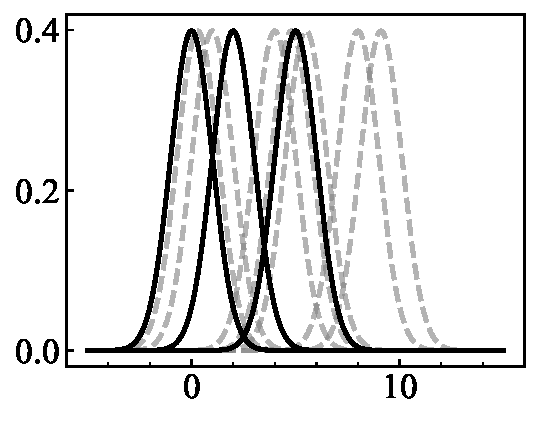
\includegraphics[width=\textwidth]{FCF_V0}
		\caption{Trọng tâm khởi tạo}
	\end{subfigure}
	\begin{subfigure}{.32\textwidth}
		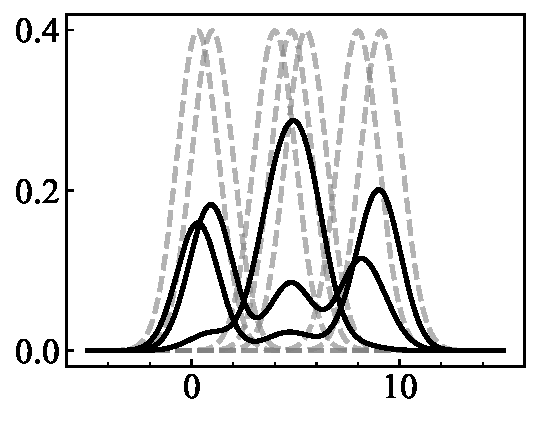
\includegraphics[width=\textwidth]{FCF_V1}
		\caption{Trọng tâm vòng lặp $t=1$}
	\end{subfigure}
		\begin{subfigure}{.32\textwidth}
		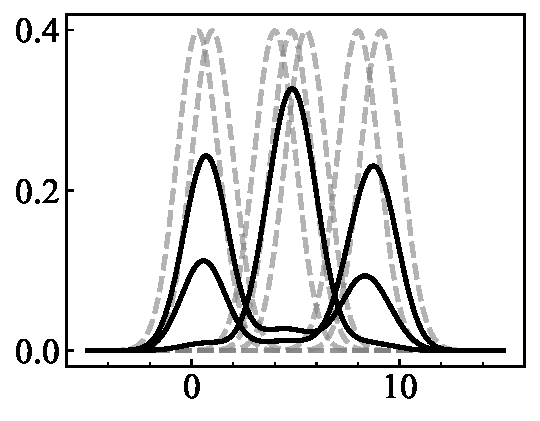
\includegraphics[width=\textwidth]{FCF_V2}
		\caption{Trọng tâm vòng lặp $t=2$}
	\end{subfigure}\hfil\\
		\begin{subfigure}{.32\textwidth}
		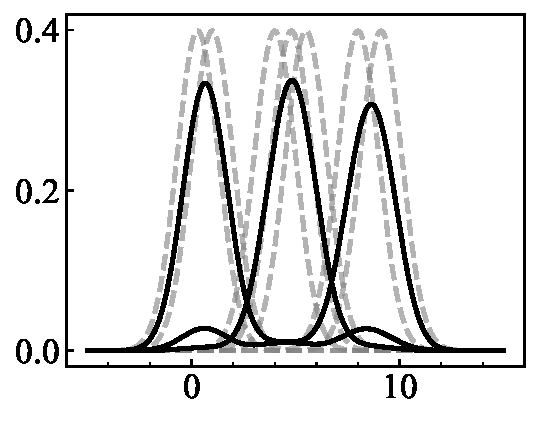
\includegraphics[width=\textwidth]{FCF_V3}
		\caption{Trọng tâm vòng lặp $t=3$}
	\end{subfigure}
	\begin{subfigure}{.32\textwidth}
		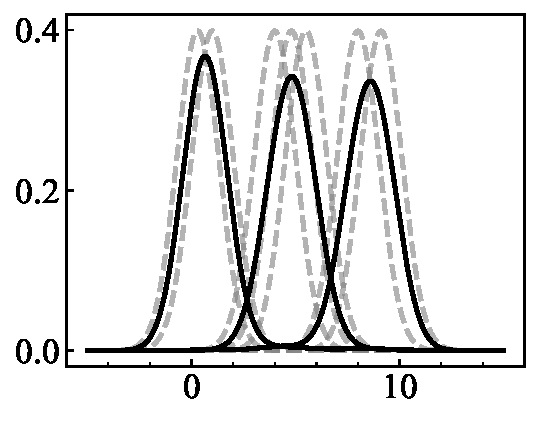
\includegraphics[width=\textwidth]{FCF_V4}
		\caption{Trọng tâm vòng lặp $t=4$}
	\end{subfigure}
	\begin{subfigure}{.32\textwidth}
		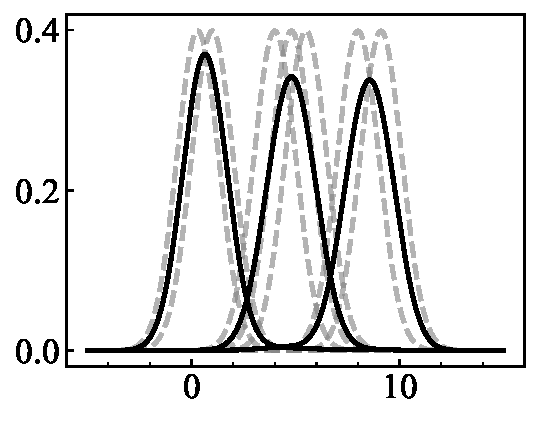
\includegraphics[width=\textwidth]{FCF_V9}
		\caption{Trọng tâm vòng lặp $t=9$}
	\end{subfigure}
	\caption{Thay đổi của trọng tâm chùm FCF qua các vòng lặp}\label{fig:vdu:trongtamFCF}
\end{figure}












\chapter*{PHỤ LỤC  C\\LÝ THUYẾT BỔ SUNG}\label{phulucC}

\begin{table}[H]
	\centering
	\caption{Một số hàm cơ sở $\psi_m(x)$ phổ biến trong hồi quy logistic cho dữ liệu hàm mật độ}
	\label{tab:basis_functions}
	\footnotesize
	\begin{tabular*}{\linewidth}{@{\extracolsep\fill}lll@{\extracolsep\fill}}
		\toprule
		\textbf{Hàm cơ sở} & \textbf{Công thức $\psi_m(x)$} & \textbf{Miền xác định} \\
		\midrule
		Gaussian (RBF) &
		$ \psi_m(x) = \exp\!\left(-\frac{(x - \mu_m)^2}{2\sigma_m^2}\right)$ &
		$x \in \mathbb{R}$ \\
		
		Hàm sóng con (Wavelet) &
		$\displaystyle \psi_m(x) = 2^{j_m/2} \, \psi\!\left(2^{j_m} x - k_m\right)$ &
		$x \in \mathbb{R}$ \\
		
		{Chuỗi Fourier} &
		$ \psi_{m}^{(\cos)}(x) = \cos\!\left(\frac{2\pi m x}{T}\right)$, \quad
		$ \psi_{m}^{(\sin)}(x) = \sin\!\left(\frac{2\pi m x}{T}\right)$ &
		$x \in [0,T]$ \\
		
		{Đa thức Bernstein} &
		$ \psi_m(x) = \binom{n}{m} x^{m} (1-x)^{n-m}$ &
		$x \in [0,1]$ \\
		
		{Đa thức Legendre} &
		$ \psi_m(x) = \frac{1}{2^{m} m!} \frac{\mathrm{d}^m}{\mathrm{d}x^m} \left[(x^2 - 1)^{m}\right]$ &
		$x \in [-1,1]$ \\
		
		{B-spline} &
		$ \psi_m(x) = \frac{x - t_m}{t_{m+k} - t_m} \, \psi_{m,k-1}(x) +
		\frac{t_{m+k+1} - x}{t_{m+k+1} - t_{m+1}} \, \psi_{m+1,k-1}(x)$, &
		$x \in \mathbb{R}$ \\
		& với $\psi_{m,0}(x) = \bm{1}_{[t_m, t_{m+1})}(x)$ &
		\\
		\bottomrule
	\end{tabular*}
\end{table}


\begin{algorithm}[H]
	\footnotesize
	\caption{Giải thuật phân tích chùm (KCF)}
	\label{alg:KCF}
	\begin{algorithmic}[1] % The number tells where the line numbering should start
		\Procedure{KCF}{$c\,;\varepsilon$}\Comment{Cho trước số chùm $c$}
		\State $t\gets0$
		\State Khởi tạo ${\bm\mu}^{(t)}$ và $\Theta^{(t)}$ ngẫu nhiên
		\While{$\Vert J^{(t+1)} - J^{(t)} \Vert<\varepsilon$}
		\State $t \gets t+1$
		\State Cập nhật ${\bm\mu}^{(t+1)}$ bằng Công thức  $\mu_{ij}= \bm 1_{\{j\in c_i\}}$
		\State Cập nhật $\Theta^{(t+1)}$ bằng Công thức \eqref{daidien_KM2}
		\EndWhile
		\State \textbf{return} ${\bm\mu}$ và $\Theta$.\Comment{Ma trận phân vùng và hàm mật độ đại diện}
		\EndProcedure
	\end{algorithmic}
\end{algorithm}


\begin{algorithm}
	\footnotesize
	\caption{Giải thuật phân chùm thứ bậc tích tụ (HCF)}\label{alg:HCF}
	\begin{algorithmic}[1]
		\Procedure{HCF}{$\mathcal{F}\,;\Delta$}\Comment{Cho trước liên kết}
				\State $t \gets 0$
		\State Khởi tạo: $\mathcal{F}^{(t=0)} = \{\{f_1\}\,;\{f_2\}\,;\ldots\,;\{f_n\}\}$
		\While{$n - t > 1$}
		\State Chọn hai $c_i\,; c_j \in \mathcal{F}^{(t=0)}$ sao cho thỏa tại vị trí $(c_i\,;c_j)=\arg\min_{c_u\,;c_v\in\mathcal{F}^{(t=0)}}\Delta(c_u\,;c_v).$
		\State Gộp $c \gets c_i \cup c_j$
		\State Cập nhật $\mathcal{F}^{t+1}\gets \left(\mathcal{F}^{(t)}\setminus\{c_i\,;c_j\}\right)\cup\{c\}$
		\State $t \gets t + 1$
		\EndWhile
		\State \textbf{return} Cây phân cấp
		\EndProcedure
	\end{algorithmic}
\end{algorithm}

\begin{algorithm}[H]
	\footnotesize
	\caption{Giải thuật phân tích chùm mờ (FCF)}
	\label{alg:FCF}
	\begin{algorithmic}[1] % The number tells where the line numbering should start
		\Procedure{FCF}{$c\,;\varepsilon$}\Comment{Cho trước số chùm $c$}
		\State $t\gets0$
		\State Khởi tạo ${\bm\mu}^{(t)}$ và $\Theta^{(t)}$ ngẫu nhiên
		\While{$\Vert {\bm\mu}^{(t+1)} - {\bm\mu}^{(t)} \Vert<\varepsilon$}
		\State $t \gets t+1$
		\State Cập nhật $\Theta^{(t+1)}$ bằng Công thức~\eqref{trongtamFCF}
		\State Cập nhật ${\bm\mu}^{(t+1)}$ bằng Công thức~\eqref{pvFCF1} và \eqref{pvFCF2}
		\EndWhile\label{euclidendwhile}
		\State \textbf{return} ${\bm\mu}$ và $\Theta$.\Comment{Ma trận phân vùng và hàm mật độ đại diện}
		\EndProcedure
	\end{algorithmic}
\end{algorithm}

\begin{algorithm}[H]
	\footnotesize
	\caption{Giải thuật phân tích chùm mờ cải tiến (IFCF)}
	\label{alg:IFCF}
	\begin{algorithmic}[1]
		\Procedure{IFCF}{$c\,;\varepsilon$}\Comment{Cho trước số chùm $c$}
		\State $t\gets0$
		\State Khởi tạo ${\bm\mu}^{(t)}$ và $\Theta^{(t)}$ ngẫu nhiên và $\omega_i^{(t)} = \bm 0$
		\While{$\Vert {\bm\mu}^{(t+1)} - {\bm\mu}^{(t)} \Vert<\varepsilon$}
		\State $t \gets t+1$
		\State Cập nhật $\Theta^{(t+1)}$ bằng Công thức~\eqref{eq:theta_update}
		\State Cập nhật ${\bm\mu}^{(t+1)}$ bằng Công thức~\eqref{eq:ifcf_u_final} và \eqref{c1_pro}
		\State Tính $\omega_i^{(t+1)} \gets \frac{1}{n}\sum_{j=1}^n \mu_{ij}^{(t+1)}$, \quad $1\le i\le c$
		\EndWhile
		\State \textbf{return} ${\bm\mu}$, $\Theta$, và $\bm\omega$.\Comment{Ma trận phân vùng, hàm mật độ đại diện, trọng số chùm}
		\EndProcedure
	\end{algorithmic}
\end{algorithm}








%\begin{figure}[H]
%    \centering
%         \centering
%\includegraphics[width=.6\textwidth]{Figs/C1_VD1_0.eps}
%       \caption{Trọng tâm $\theta^{(0)}$ được khởi tạo từ ${\bm\mu}^{(0)}$}
%   \end{figure}

%\begin{figure}[H]
%     \centering
%     \begin{subfigure}[b]{0.31\textwidth}
%         \centering
%         \includegraphics[width=\textwidth]{Figs/C1_VD1_1.eps}
%         \caption{Vòng lặp 1}
%     \end{subfigure}
%     \hfill
%     \begin{subfigure}[b]{0.31\textwidth}
%         \centering
%        \includegraphics[width=\textwidth]{Figs/C1_VD1_2.eps}
%         \caption{Vòng lặp 2}
%     \end{subfigure}
%     \hfill
%     \begin{subfigure}[b]{0.31\textwidth}
%         \centering
%         \includegraphics[width=\textwidth]{Figs/C1_VD1_3.eps}
%         \caption{Vòng lặp 3}
%     \end{subfigure}
%    \begin{subfigure}[b]{0.31\textwidth}
%        \centering
%         \includegraphics[width=\textwidth]{Figs/C1_VD1_6.eps}
%         \caption{Vòng lặp 6}
%     \end{subfigure}
%     \hfill
%     \begin{subfigure}[b]{0.31\textwidth}
%         \centering
%         \includegraphics[width=\textwidth]{Figs/C1_VD1_7.eps}
%         \caption{Vòng lặp 7}
%     \end{subfigure}
%     \hfill
%     \begin{subfigure}[b]{0.31\textwidth}
%         \centering
%         \includegraphics[width=\textwidth]{Figs/C1_VD1_8.eps}
%         \caption{Vòng lặp 8}
%     \end{subfigure}
%        \caption{Sự thay đổi qua các vòng lặp trong thuật toán FCF}
%        \label{fig:VD1}
%\end{figure}



%\chapter*{XÁC NHẬN CỦA HỘI ĐỒNG}
%
%\begin{center}
%	\begin{tabular*}{.7\columnwidth}{@{\extracolsep\fill}cc@{\extracolsep\fill}} 
%		\textbf{Cán bộ hướng dẫn} & \textbf{Học viên thực hiện}\\
%		\textit{(Ký tên)} & \textit{(Ký tên)}\\
%\end{tabular*}
%\end{center}



\addcontentsline{toc}{chapter}{\numberline{CHỈ MỤC}}%
\printindex



\end{document}